\documentclass[10pt,a4paper,onecolumn]{article}
\usepackage{marginnote}
\usepackage{zref-savepos}
\usepackage{graphicx}
\usepackage{xcolor}
\usepackage{authblk,etoolbox}
\usepackage{titlesec}
\usepackage{calc}
\usepackage{tikz}
\usepackage{hyperref}
\hypersetup{colorlinks,breaklinks=true,
            urlcolor=[rgb]{0.0, 0.5, 1.0},
            linkcolor=[rgb]{0.0, 0.5, 1.0}}
\usepackage{caption}
\usepackage{array}
\usepackage{tcolorbox}
\usepackage{amssymb,amsmath}
\usepackage{ifxetex,ifluatex}
\usepackage{seqsplit}
\usepackage{xstring}
\usepackage{ifluatex}
\ifluatex
  \usepackage{fontspec}
\else
  \usepackage[T1]{fontenc}
\fi
\usepackage{lmodern}
\usepackage{colortbl}
\usepackage{tabularx}
\usepackage{fontawesome5}
% \usepackage{textpos}

\usepackage{float}
\let\origfigure\figure
\let\endorigfigure\endfigure
\renewenvironment{figure}[1][2] {
    \expandafter\origfigure\expandafter[H]
} {
    \endorigfigure
}

\usepackage{fixltx2e} % provides \textsubscript
\usepackage[
  backend=biber,
  style=apa,
]{biblatex}
\bibliography{paper.bib}
% Match the heading style/level pandoc used for References previously
\defbibheading{bibliography}{%
  \subsection*{References}\label{references}%
  \addcontentsline{toc}{subsection}{References}%
}

% --- CiTO annotations for the biblatex-rendered bibliography -----------------
% resources/biohackrxiv/filters/cito-to-biblatex.lua turns the CiTO
% properties collected by extract-cito.lua into \citoannotate{key}{property}
% calls; this hook accumulates them per entry key and prints them at the end
% of each bibliography entry via biblatex's "finentry" bibmacro, which every
% entry-type driver (including biblatex-apa's) invokes to close the entry.
\makeatletter
\newcommand{\citoannotate}[2]{%
  \expandafter\ifx\csname cito@#1\endcsname\relax
    \expandafter\gdef\csname cito@#1\endcsname{\textbf{\ [cito:#2]}}%
  \else
    \expandafter\g@addto@macro\csname cito@#1\endcsname{\textbf{\ [cito:#2]}}%
  \fi
}
\newcommand{\printcitoannotation}{%
  \@ifundefined{cito@\strfield{entrykey}}{}{\csname cito@\strfield{entrykey}\endcsname}%
}
\makeatother
\renewbibmacro*{finentry}{\printcitoannotation\finentry}

% --- Splitting \texttt --------------------------------------------------

\let\textttOrig=\texttt
\def\texttt#1{\expandafter\textttOrig{\seqsplit{#1}}}
\renewcommand{\seqinsert}{\ifmmode
  \allowbreak
  \else\penalty6000\hspace{0pt plus 0.02em}\fi}


% --- Pandoc does not distinguish between links like [foo](bar) and
% --- [foo](foo) -- a simplistic Markdown model.  However, this is
% --- wrong:  in links like [foo](foo) the text is the url, and must
% --- be split correspondingly.
% --- Here we detect links \href{foo}{foo}, and also links starting
% --- with https://doi.org, and use path-like splitting (but not
% --- escaping!) with these links.
% --- Another vile thing pandoc does is the different escaping of
% --- foo and bar.  This may confound our detection.
% --- This problem we do not try to solve at present, with the exception
% --- of doi-like urls, which we detect correctly.


\makeatletter
\let\href@Orig=\href
\def\href@Urllike#1#2{\href@Orig{#1}{\begingroup
    \def\Url@String{#2}\Url@FormatString
    \endgroup}}
\def\href@Notdoi#1#2{\def\tempa{#1}\def\tempb{#2}%
  \ifx\tempa\tempb\relax\href@Urllike{#1}{#2}\else
  \href@Orig{#1}{#2}\fi}
\def\href#1#2{%
  \IfBeginWith{#1}{https://doi.org}%
  {\href@Urllike{#1}{#2}}{\href@Notdoi{#1}{#2}}}
% biblatex-apa's own "doi+url" bibmacro calls \href{https://doi.org/...}
% {\nolinkurl{...}} while printing each entry; the override above assumes
% its second argument is a plain string matching the URL (true for
% pandoc-authored markdown links, not for \nolinkurl's macro call), and
% feeding that into \Url@FormatString crashes with a math-mode error. Same
% fix as \affil's \let\href=\href@Orig below: bypass the override there.
\AtBeginBibliography{\let\href\href@Orig}
\makeatother


% --- Page layout -------------------------------------------------------------
\usepackage[top=3.5cm, bottom=3cm, right=1.5cm, left=1.0cm,
            headheight=2.2cm, reversemp, includemp, marginparwidth=4.5cm]{geometry}
% \renewcommand{\marginnotevadjust}{-2in}

% --- Default font ------------------------------------------------------------
\renewcommand\familydefault{\sfdefault}

% --- Style -------------------------------------------------------------------
\renewcommand{\bibfont}{\small \sffamily}
\renewcommand{\captionfont}{\small\sffamily}
\renewcommand{\captionlabelfont}{\bfseries}

% --- Section/SubSection/SubSubSection ----------------------------------------
\titleformat{\section}
  {\normalfont\sffamily\Large\bfseries}
  {}{0pt}{}
\titleformat{\subsection}
  {\normalfont\sffamily\large\bfseries}
  {}{0pt}{}
\titleformat{\subsubsection}
  {\normalfont\sffamily\bfseries}
  {}{0pt}{}
\titleformat*{\paragraph}
  {\sffamily\normalsize}


% --- Header / Footer ---------------------------------------------------------
\usepackage{fancyhdr}
\pagestyle{fancy}
\fancyhf{}
%\renewcommand{\headrulewidth}{0.50pt}
\renewcommand{\headrulewidth}{0pt}
\fancyhead[L]{\hspace{-0.75cm}
\includegraphics[width=5.5cm]{logo.png}}
\fancyhead[C]{}
\fancyhead[R]{}
\renewcommand{\footrulewidth}{0.25pt}

\fancyfoot[L]{\parbox[t]{0.98\headwidth}{\footnotesize{\sffamily Kawashima
\emph{et al.},  (2026). {\href{https://biohackrxiv.org/}{BioHackrXiv.org}}}}}
%      \textit{\url{https://biohackrxiv.org/}{BioHackrXiv.org}}}}


\fancyfoot[R]{\sffamily \thepage}
\makeatletter
\let\ps@plain\ps@fancy
\fancyheadoffset[L]{4.5cm}
\fancyfootoffset[L]{4.5cm}

% --- Macros ---------

\definecolor{linky}{rgb}{0.0, 0.5, 1.0}

\newtcolorbox{repobox}
   {colback=red, colframe=red!75!black,
     boxrule=0.5pt, arc=2pt, left=6pt, right=6pt, top=3pt, bottom=3pt}

\newcommand{\ExternalLink}{%
   \tikz[x=1.2ex, y=1.2ex, baseline=-0.05ex]{%
       \begin{scope}[x=1ex, y=1ex]
           \clip (-0.1,-0.1)
               --++ (-0, 1.2)
               --++ (0.6, 0)
               --++ (0, -0.6)
               --++ (0.6, 0)
               --++ (0, -1);
           \path[draw,
               line width = 0.5,
               rounded corners=0.5]
               (0,0) rectangle (1,1);
       \end{scope}
       \path[draw, line width = 0.5] (0.5, 0.5)
           -- (1, 1);
       \path[draw, line width = 0.5] (0.6, 1)
           -- (1, 1) -- (1, 0.6);
       }
   }

% --- Title / Authors ---------------------------------------------------------
% patch \maketitle so that it doesn't center
\patchcmd{\@maketitle}{center}{flushleft}{}{}
\patchcmd{\@maketitle}{center}{flushleft}{}{}
% patch \maketitle so that the font size for the title is normal
\patchcmd{\@maketitle}{\HUGE}{\HUGE\sffamily}{}{}
% patch the patch by authblk so that the author block is flush left
\def\maketitle{{%
  \renewenvironment{tabular}[2][]
    {\zsavepos{authortop}\begin{flushleft}}
    {\end{flushleft}}
  \AB@maketitle}}
\makeatletter
\renewcommand\AB@affilsepx{ \protect\Affilfont}
%\renewcommand\AB@affilnote[1]{{\bfseries #1}\hspace{2pt}}
\renewcommand\AB@affilnote[1]{{\bfseries #1}\hspace{3pt}}
\renewcommand{\affil}[2][]%
   {\newaffiltrue\let\AB@blk@and\AB@pand
      \if\relax#1\relax\def\AB@note{\AB@thenote}\else\def\AB@note{#1}%
        \setcounter{Maxaffil}{0}\fi
        \begingroup
        \let\href=\href@Orig
        \let\texttt=\textttOrig
        \let\protect\@unexpandable@protect
        \def\thanks{\protect\thanks}\def\footnote{\protect\footnote}%
        \@temptokena=\expandafter{\AB@authors}%
        {\def\\{\protect\\\protect\Affilfont}\xdef\AB@temp{#2}}%
         \xdef\AB@authors{\the\@temptokena\AB@las\AB@au@str
         \protect\\[\affilsep]\protect\Affilfont\AB@temp}%
         \gdef\AB@las{}\gdef\AB@au@str{}%
        {\def\\{, \ignorespaces}\xdef\AB@temp{#2}}%
        \@temptokena=\expandafter{\AB@affillist}%
        \xdef\AB@affillist{\the\@temptokena \AB@affilsep
          \AB@affilnote{\AB@note}\protect\Affilfont\AB@temp}%
      \endgroup
       \let\AB@affilsep\AB@affilsepx
}
\makeatother
\renewcommand\Authfont{\sffamily\bfseries}
\renewcommand\Affilfont{\sffamily\small\mdseries}
\setlength{\affilsep}{1em}


\ifnum 0\ifxetex 1\fi\ifluatex 1\fi=0 % if pdftex
  \usepackage[T1]{fontenc}
  \usepackage[utf8]{inputenc}

\else % if luatex or xelatex
  \ifxetex
    \usepackage{mathspec}
    \usepackage{fontspec}

  \else
    \usepackage{fontspec}
  \fi
  \defaultfontfeatures{Ligatures=TeX,Scale=MatchLowercase}
  % CJK and extended Unicode support via Noto fonts
  \usepackage{luaotfload}
  \directlua{luaotfload.add_fallback("cjkfallback",
    {"NotoSansCJKsc:style=Regular;","NotoSerifCJKsc:style=Regular;"}
  )}
  \setmainfont{Latin Modern Roman}[RawFeature={fallback=cjkfallback}]
  \setsansfont{Latin Modern Sans}[RawFeature={fallback=cjkfallback}]

\fi
% use upquote if available, for straight quotes in verbatim environments
\IfFileExists{upquote.sty}{\usepackage{upquote}}{}
% use microtype if available
\IfFileExists{microtype.sty}{%
\usepackage{microtype}
\UseMicrotypeSet[protrusion]{basicmath} % disable protrusion for tt fonts
}{}

\usepackage{hyperref}
\hypersetup{unicode=true,
            pdftitle={Predicting microbial energy metabolism from genomes through knowledge graphs and machine learning},
            pdfborder={0 0 0},
            breaklinks=true}
\urlstyle{same}  % don't use monospace font for urls
\usepackage{biblatex}

\addbibresource{paper.bib}
\usepackage{longtable,booktabs}

% --- We redefined \texttt, but in sections and captions we want the
% --- old definition
\let\addcontentslineOrig=\addcontentsline
\def\addcontentsline#1#2#3{\bgroup
  \let\texttt=\textttOrig\addcontentslineOrig{#1}{#2}{#3}\egroup}
\let\markbothOrig\markboth
\def\markboth#1#2{\bgroup
  \let\texttt=\textttOrig\markbothOrig{#1}{#2}\egroup}
\let\markrightOrig\markright
\def\markright#1{\bgroup
  \let\texttt=\textttOrig\markrightOrig{#1}\egroup}


\usepackage{graphicx,grffile}
\makeatletter
\def\maxwidth{\ifdim\Gin@nat@width>\linewidth\linewidth\else\Gin@nat@width\fi}
\def\maxheight{\ifdim\Gin@nat@height>\textheight\textheight\else\Gin@nat@height\fi}
\makeatother
% Scale images if necessary, so that they will not overflow the page
% margins by default, and it is still possible to overwrite the defaults
% using explicit options in \includegraphics[width, height, ...]{}
\setkeys{Gin}{width=\maxwidth,height=\maxheight,keepaspectratio}
\IfFileExists{parskip.sty}{%
\usepackage{parskip}
}{% else
\setlength{\parindent}{0pt}
\setlength{\parskip}{6pt plus 2pt minus 1pt}
}
\setlength{\emergencystretch}{3em}  % prevent overfull lines
\providecommand{\tightlist}{%
  \setlength{\itemsep}{0pt}\setlength{\parskip}{0pt}}
% Pandoc 3.x image scaling support
\makeatletter
\newsavebox\pandoc@box
\newcommand*\pandocbounded[1]{%
  \sbox\pandoc@box{#1}%
  \Gscale@div\@tempa{\textheight}{\dimexpr\ht\pandoc@box+\dp\pandoc@box\relax}%
  \Gscale@div\@tempb{\linewidth}{\wd\pandoc@box}%
  \ifdim\@tempb\p@<\@tempa\p@\let\@tempa\@tempb\fi%
  \ifdim\@tempa\p@<\p@\scalebox{\@tempa}{\usebox\pandoc@box}%
  \else\usebox{\pandoc@box}%
  \fi%
}
\makeatother
\setcounter{secnumdepth}{0}
% Redefines (sub)paragraphs to behave more like sections
\ifx\paragraph\undefined\else
\let\oldparagraph\paragraph
\renewcommand{\paragraph}[1]{\oldparagraph{#1}\mbox{}}
\fi
\ifx\subparagraph\undefined\else
\let\oldsubparagraph\subparagraph
\renewcommand{\subparagraph}[1]{\oldsubparagraph{#1}\mbox{}}
\fi

\newcommand{\fillin}[1]{\textcolor{red}{[#1]}}

\title{Predicting microbial energy metabolism from genomes through
knowledge graphs and machine learning}

% ORCID support

\definecolor{orcidlogocol}{HTML}{A6CE39}
\newcommand{\orcidlink}[1]{\protect\href{https://orcid.org/#1}{\,\small\textcolor{orcidlogocol}{\faOrcid}\,}}

% ROR support

% Based on work by Charles Tapley Hoyt <https://github.com/cthoyt>. See https://github.com/openjournals/inara/pull/72
\definecolor{c53baa1}{RGB}{83,186,161}
\definecolor{c202826}{RGB}{32,40,38}
\def \rorglobalscale {0.1}
\newcommand{\rorlogo}{%
\begin{tikzpicture}[y=1cm, x=1cm, yscale=\rorglobalscale,xscale=\rorglobalscale, every node/.append style={scale=\rorglobalscale}, inner sep=0pt, outer sep=0pt]
  \begin{scope}[even odd rule,line join=round,miter limit=2.0,shift={(-0.025, 0.0216)}]
    \path[fill=c53baa1,nonzero rule,line join=round,miter limit=2.0] (1.8164, 3.012) -- (1.4954, 2.5204) -- (1.1742, 3.012) -- (1.8164, 3.012) -- cycle;
    \path[fill=c53baa1,nonzero rule,line join=round,miter limit=2.0] (3.1594, 3.012) -- (2.8385, 2.5204) -- (2.5172, 3.012) -- (3.1594, 3.012) -- cycle;
    \path[fill=c53baa1,nonzero rule,line join=round,miter limit=2.0] (1.1742, 0.0669) -- (1.4954, 0.5588) -- (1.8164, 0.0669) -- (1.1742, 0.0669) -- cycle;
    \path[fill=c53baa1,nonzero rule,line join=round,miter limit=2.0] (2.5172, 0.0669) -- (2.8385, 0.5588) -- (3.1594, 0.0669) -- (2.5172, 0.0669) -- cycle;
    \path[fill=c202826,nonzero rule,line join=round,miter limit=2.0] (3.8505, 1.4364).. controls (3.9643, 1.4576) and (4.0508, 1.5081) .. (4.1098, 1.5878).. controls (4.169, 1.6674) and (4.1984, 1.7642) .. (4.1984, 1.8777).. controls (4.1984, 1.9719) and (4.182, 2.0503) .. (4.1495, 2.1132).. controls (4.1169, 2.1762) and (4.0727, 2.2262) .. (4.0174, 2.2635).. controls (3.9621, 2.3006) and (3.8976, 2.3273) .. (3.824, 2.3432).. controls (3.7505, 2.359) and (3.6727, 2.367) .. (3.5909, 2.367) -- (2.9676, 2.367) -- (2.9676, 1.8688).. controls (2.9625, 1.8833) and (2.9572, 1.8976) .. (2.9514, 1.9119).. controls (2.9083, 2.0164) and (2.848, 2.1056) .. (2.7705, 2.1791).. controls (2.6929, 2.2527) and (2.6014, 2.3093) .. (2.495, 2.3487).. controls (2.3889, 2.3881) and (2.2728, 2.408) .. (2.1468, 2.408).. controls (2.0209, 2.408) and (1.905, 2.3881) .. (1.7986, 2.3487).. controls (1.6925, 2.3093) and (1.6007, 2.2527) .. (1.5232, 2.1791).. controls (1.4539, 2.1132) and (1.3983, 2.0346) .. (1.3565, 1.9436).. controls (1.3504, 2.009) and (1.3351, 2.0656) .. (1.3105, 2.1132).. controls (1.2779, 2.1762) and (1.2338, 2.2262) .. (1.1785, 2.2635).. controls (1.1232, 2.3006) and (1.0586, 2.3273) .. (0.985, 2.3432).. controls (0.9115, 2.359) and (0.8337, 2.367) .. (0.7519, 2.367) -- (0.1289, 2.367) -- (0.1289, 0.7562) -- (0.4837, 0.7562) -- (0.4837, 1.4002) -- (0.6588, 1.4002) -- (0.9956, 0.7562) -- (1.4211, 0.7562) -- (1.0118, 1.4364).. controls (1.1255, 1.4576) and (1.2121, 1.5081) .. (1.2711, 1.5878).. controls (1.2737, 1.5915) and (1.2761, 1.5954) .. (1.2787, 1.5991).. controls (1.2782, 1.5867) and (1.2779, 1.5743) .. (1.2779, 1.5616).. controls (1.2779, 1.4327) and (1.2996, 1.3158) .. (1.3428, 1.2113).. controls (1.3859, 1.1068) and (1.4462, 1.0176) .. (1.5237, 0.944).. controls (1.601, 0.8705) and (1.6928, 0.8139) .. (1.7992, 0.7744).. controls (1.9053, 0.735) and (2.0214, 0.7152) .. (2.1474, 0.7152).. controls (2.2733, 0.7152) and (2.3892, 0.735) .. (2.4956, 0.7744).. controls (2.6016, 0.8139) and (2.6935, 0.8705) .. (2.771, 0.944).. controls (2.8482, 1.0176) and (2.9086, 1.1068) .. (2.952, 1.2113).. controls (2.9578, 1.2253) and (2.9631, 1.2398) .. (2.9681, 1.2544) -- (2.9681, 0.7562) -- (3.3229, 0.7562) -- (3.3229, 1.4002) -- (3.4981, 1.4002) -- (3.8349, 0.7562) -- (4.2603, 0.7562) -- (3.8505, 1.4364) -- cycle(0.9628, 1.7777).. controls (0.9438, 1.7534) and (0.92, 1.7357) .. (0.8911, 1.7243).. controls (0.8623, 1.7129) and (0.83, 1.706) .. (0.7945, 1.7039).. controls (0.7588, 1.7015) and (0.7252, 1.7005) .. (0.6932, 1.7005) -- (0.4839, 1.7005) -- (0.4839, 2.0667) -- (0.716, 2.0667).. controls (0.7477, 2.0667) and (0.7805, 2.0643) .. (0.8139, 2.0598).. controls (0.8472, 2.0553) and (0.8768, 2.0466) .. (0.9025, 2.0336).. controls (0.9282, 2.0206) and (0.9496, 2.0021) .. (0.9663, 1.9778).. controls (0.9829, 1.9534) and (0.9914, 1.9209) .. (0.9914, 1.8799).. controls (0.9914, 1.8362) and (0.9819, 1.8021) .. (0.9628, 1.7777) -- cycle(2.6125, 1.3533).. controls (2.5889, 1.2904) and (2.5553, 1.2359) .. (2.5112, 1.1896).. controls (2.4672, 1.1433) and (2.4146, 1.1073) .. (2.3529, 1.0814).. controls (2.2916, 1.0554) and (2.2228, 1.0427) .. (2.1471, 1.0427).. controls (2.0712, 1.0427) and (2.0026, 1.0557) .. (1.9412, 1.0814).. controls (1.8799, 1.107) and (1.8272, 1.1433) .. (1.783, 1.1896).. controls (1.7391, 1.2359) and (1.7052, 1.2904) .. (1.6817, 1.3533).. controls (1.6581, 1.4163) and (1.6465, 1.4856) .. (1.6465, 1.5616).. controls (1.6465, 1.6359) and (1.6581, 1.705) .. (1.6817, 1.7687).. controls (1.7052, 1.8325) and (1.7388, 1.8873) .. (1.783, 1.9336).. controls (1.8269, 1.9799) and (1.8796, 2.0159) .. (1.9412, 2.0418).. controls (2.0026, 2.0675) and (2.0712, 2.0804) .. (2.1471, 2.0804).. controls (2.223, 2.0804) and (2.2916, 2.0675) .. (2.3529, 2.0418).. controls (2.4143, 2.0161) and (2.467, 1.9799) .. (2.5112, 1.9336).. controls (2.5551, 1.8873) and (2.5889, 1.8322) .. (2.6125, 1.7687).. controls (2.636, 1.705) and (2.6477, 1.6359) .. (2.6477, 1.5616).. controls (2.6477, 1.4856) and (2.636, 1.4163) .. (2.6125, 1.3533) -- cycle(3.8015, 1.7777).. controls (3.7825, 1.7534) and (3.7587, 1.7357) .. (3.7298, 1.7243).. controls (3.701, 1.7129) and (3.6687, 1.706) .. (3.6333, 1.7039).. controls (3.5975, 1.7015) and (3.5639, 1.7005) .. (3.5319, 1.7005) -- (3.3226, 1.7005) -- (3.3226, 2.0667) -- (3.5547, 2.0667).. controls (3.5864, 2.0667) and (3.6192, 2.0643) .. (3.6526, 2.0598).. controls (3.6859, 2.0553) and (3.7155, 2.0466) .. (3.7412, 2.0336).. controls (3.7669, 2.0206) and (3.7883, 2.0021) .. (3.805, 1.9778).. controls (3.8216, 1.9534) and (3.8301, 1.9209) .. (3.8301, 1.8799).. controls (3.8301, 1.8362) and (3.8206, 1.8021) .. (3.8015, 1.7777) -- cycle;
  \end{scope}
\end{tikzpicture}
}

\newcommand{\rorlink}[1]{\,\href{https://ror.org/#1}{\protect\rorlogo}}

        \author[1]{Shuichi Kawashima\orcidlink{0000-0001-7883-3756}}
          \author[2]{Danil Ezhov\orcidlink{0000-0002-5548-6103}}
          \author[3]{Akira R Kinjo\orcidlink{0000-0002-4006-8208}}
          \author[4]{Julia Koblitz\orcidlink{0000-0002-7260-2129}}
          \author[5]{Takeru Nakazato\orcidlink{0000-0002-0706-2867}}
          \author[6]{Yoko Okabbepu\orcidlink{0000-0000-0000-0000}}
          \author[5]{Risa Otsuka\orcidlink{0000-0000-0000-0000}}
    
      \affil[1]{Database Division for Life Science, BioData Science
Initiative, National Institute of Genetics, Research Organization of
Information and Systems, Chiba, Japan}
      \affil[2]{ITMO University, Russia\rorlink{044rwnt51}}
      \affil[3]{Anima Machina G.K., Osaka, Japan\rorlink{044rwnt51}}
      \affil[4]{OSIRIS Solutions GmbH, Germany\rorlink{044rwnt51}}
      \affil[5]{Biological Resource Center, National Institute of
Technology and Evaluation, Japan\rorlink{044rwnt51}}
      \affil[6]{OKBP Inc., Japan\rorlink{044rwnt51}}
  \date{\vspace{-7ex}}

% pdfLaTeX fallback: the project is built with LuaLaTeX; these lines let main.tex also compile with pdfLaTeX
\ifnum 0\ifxetex 1\fi\ifluatex 1\fi=0
  \DeclareUnicodeCharacter{2212}{\ensuremath{-}}
  \DeclareUnicodeCharacter{2020}{\ensuremath{\dagger}}
  \DeclareUnicodeCharacter{2265}{\ensuremath{\geq}}
  \DeclareUnicodeCharacter{2264}{\ensuremath{\leq}}
  \DeclareUnicodeCharacter{00D7}{\ensuremath{\times}}
\fi

\begin{document}


\maketitle

\zsavepos{marginnoteanchor}
\marginnote{

   \begin{flushleft}
   \sffamily\small

  {\bfseries BioHackathon series:} \\
  \href{https://2026.biohackathon.org/}{\color{linky}{DBCLS BioHackathon 2026}} \\
       {Matsuyama, Japan, 2026} \\

  % \vspace{2mm}

  % {\bfseries Group:} \\
    \emph{\href{https://github.com/biohackathon-japan/BH26-microbial-metabolic-traits}{microbial-metabolic-traits}} \\

  \vspace{2mm}

%  {\bfseries Software}
%  \begin{itemize}
%    \setlength\itemsep{0em}
%    \item \href{}{\color{linky}{Repository}} \ExternalLink
%    \item \href{}{\color{linky}{Branch}} \ExternalLink
%  \end{itemize}

  \vspace{2mm}

  {\bfseries Submitted:} 23 Oct 2026
  %  {\bfseries Published:} 


  \vspace{2mm}
  {\bfseries License:}\\
  Authors retain copyright and release the work under a Creative Commons Attribution 4.0 International License (\href{https://creativecommons.org/licenses/by/4.0/}{\color{linky}{CC-BY}}).

  \vspace{4mm}

  Published by
  \href{https://biohackrxiv.org/}{\color{linky}{BioHackrXiv.org}}
  % \par\vspace*{\fill}

  \end{flushleft}
  \sffamily\small

}[\dimexpr(\zposy{marginnoteanchor}sp-\zposy{authortop}sp)\relax]




\citoannotate{Jones2014}{citesAsAuthority}

\citoannotate{Larralde2023}{citesAsAuthority}

\citoannotate{Koblitz2025}{citesAsAuthority}

\citoannotate{Nayfach2021}{citesAsAuthority}

\citoannotate{Mordelet2014}{citesAsAuthority}

\citoannotate{Madin2020}{citesAsAuthority}

\citoannotate{Davin2025}{citesAsAuthority}

\citoannotate{Roberts2017}{citesAsAuthority}

\citoannotate{FedotMAS2026}{citesAsAuthority}

\citoannotate{EvolutionaryScale2024}{citesAsAuthority}

\citoannotate{Anantharaman2016}{citesAsAuthority}

\citoannotate{Shi2016}{citesAsAuthority}

\citoannotate{Kanehisa2025}{citesAsAuthority}

\citoannotate{Huang2023}{citesAsAuthority}

\citoannotate{Zimmermann2021}{citesAsAuthority}

\citoannotate{Bowers2017}{citesAsAuthority}

\citoannotate{Zhou2022}{citesAsAuthority}

\citoannotate{Walsh2021}{citesAsAuthority}

\citoannotate{Platt1999}{citesAsAuthority}

\citoannotate{Matthews1975}{citesAsAuthority}

\citoannotate{Wiatrak2025}{citesAsAuthority}

\citoannotate{Weissman2021}{citesAsAuthority}

\citoannotate{Goberna2016}{citesAsAuthority}

\citoannotate{Vickers2006}{citesAsAuthority}

\citoannotate{Angelopoulos2023}{citesAsAuthority}

\citoannotate{Hwang2024}{citesAsAuthority}

\citoannotate{Weimann2016}{citesAsAuthority}

\citoannotate{Kinjo2026}{citesAsAuthority}

\citoannotate{Aramaki2020}{citesAsAuthority}

\citoannotate{Gartlehner2025}{citesAsAuthority}

\citoannotate{Schober2025}{citesAsAuthority}

\citoannotate{Chicco2020}{citesAsAuthority}

\citoannotate{Sauer2019}{citesAsAuthority}

\citoannotate{Greening2016}{citesAsAuthority}

\citoannotate{Flamholz2024}{citesAsAuthority}

\citoannotate{Santos2015}{citesAsAuthority}

\citoannotate{Chklovski2023}{citesAsAuthority}

\citoannotate{Saito2015}{citesAsAuthority}

\citoannotate{Parks2022}{citesAsAuthority}

\citoannotate{Hackmann2026}{citesAsAuthority}

\citoannotate{Nguyen2024}{citesAsAuthority}

\citoannotate{Lundberg2020}{citesAsAuthority}

\citoannotate{Breiman2001}{citesAsAuthority}

\citoannotate{Lin2023}{citesAsAuthority}

\citoannotate{Hyatt2010}{citesAsAuthority}

\citoannotate{Kawashima2018}{citesAsAuthority}

\citoannotate{Geurts2006}{citesAsAuthority}

\citoannotate{Douglas2020}{citesAsAuthority}

\citoannotate{Larralde2022}{citesAsAuthority}

\citoannotate{Kawashima2026}{citesAsAuthority}

\citoannotate{Brbic2016}{citesAsAuthority}

\citoannotate{Ilse2018}{citesAsAuthority}

\citoannotate{Shaffer2020}{citesAsAuthority}

\citoannotate{Hollmann2025}{citesAsAuthority}

\citoannotate{Chen2016}{citesAsAuthority}

\citoannotate{Louca2016}{citesAsAuthority}

\section{Abstract}\label{abstract}

The increasing availability of microbial genomes creates opportunities
to predict physiological traits and prioritize cultivation experiments.
During DBCLS BioHackathon 2026, we connected genome-derived protein
annotations to electron donor and acceptor information, initially
focusing on autotrophic microorganisms. KofamScan annotations for 23,434
RefSeq genomes and KEGG Orthology (KO) definitions were represented in
RDF and made accessible through TogoMCP. Literature-assisted phenotype
collection and an interactive viewer linked reported physiology to
genomic evidence. Within a focused collection of 586 genomes, 358
labeled genomes supported evaluation of 14 metabolic categories. A
KO-based classifier achieved macro area under the precision-recall curve
(AUPRC) of 0.612 when entire genera were held out, compared with 0.472
for a taxonomic baseline. Combining KO and protein language model
representations improved internal performance to 0.625, although the
contribution beyond ensembling KO-based learners was not statistically
resolved. This improvement did not transfer to external evaluation. On
562 genomes from unseen genera, the KO model achieved 0.555 versus 0.380
for the taxonomic baseline. Completeness scores for 71 KEGG modules
provided complementary pathway annotations. Performance varied
substantially among traits, and disagreement between phenotype
compilations identified priorities for further curation. These hackathon
outcomes establish a shared basis for evidence retrieval, comparative
visualization, and genome-guided screening, while experimental
validation remains necessary before predictions can guide cultivation.

\section{Introduction}\label{introduction}

Metagenomic sequencing and genome reconstruction have greatly expanded
access to microbial diversity, including lineages without cultured
representatives. Large collections of metagenome-assembled genomes
(MAGs) provide opportunities to investigate functions that would be
difficult to discover through cultivation alone \autocite{Nayfach2021}.
However, the increasing availability of sequences has not been matched
by physiological characterization. Methods that connect genomes to
experimentally relevant traits could help prioritize organisms for
screening and identify candidates with useful biochemical capabilities.

Carbon fixation provides one example of this approach. AutoFixMark uses
curated combinations of KEGG Orthology (KO) markers to infer CO2
fixation pathways from genome annotations \autocite{Kawashima2026}. Such
resources make biological knowledge usable for interpretable screening.
The ability to assimilate inorganic carbon, however, does not identify
how an organism acquires the energy and reducing power needed for
growth. Carbon assimilation and energy acquisition therefore require
complementary descriptions.

Electron donors and acceptors are central to this second question. Their
utilization describes the redox transformations through which
microorganisms can conserve energy and can inform the selection of
candidate medium components and cultivation atmospheres. We initially
focused on autotrophic microorganisms, particularly
chemolithoautotrophs, because existing carbon fixation resources offer a
practical starting point and because considering carbon supply
separately from electron donation helps formulate explicit cultivation
hypotheses. This focus does not imply that all autotrophs use
exclusively inorganic electron donors or that carbon fixation genes
alone establish autotrophic growth. Facultative lifestyles and
condition-dependent substrate use remain relevant.

Several tools already predict microbial traits from genomes. Traitar
learns protein-family signatures for 67 phenotypes from labeled isolates
\autocite{Weimann2016}, ProTraits combines text mining with comparative
genomics for several hundred traits \autocite{Brbic2016}, and FAPROTAX,
DRAM and METABOLIC assign functions from taxonomy or curated annotation
rules \autocite{Louca2016,Shaffer2020,Zhou2022}. Other predictors
estimate optimal growth temperature, maximal growth rate or oxygen use
from genome composition \autocite{Sauer2019,Weissman2021,Flamholz2024},
and metabolic reconstructions predict substrate use
\autocite{Zimmermann2021}. Classifiers trained on curated strain data
from BacDive now add predicted traits to that database
\autocite{Koblitz2025}, and Microbe Decoder offers taxonomy-based,
metabolic-network and machine-learning predictors evaluated with higher
taxonomic ranks held out \autocite{Hackmann2026}. These resources cover
respiration types and fermentation well. Electron donors used by
lithotrophs, such as hydrogen, reduced sulfur, ferrous iron, ammonia,
nitrite and carbon monoxide, are rarely predicted from gene content and
tested outside the lineages used for training.

At BioHackathon 2026, we combined data integration, literature-assisted
curation, visualization, and predictive modeling around this question.
The project addressed two related needs: enabling an AI assistant to
retrieve and explain evidence about a named organism, and evaluating
whether genome-derived features predict traits beyond labeled training
lineages. The former can draw on published physiology, whereas the
latter must be assessed under controlled conditions relevant to
uncharacterized organisms. We report the resources developed during the
hackathon, trait predictors evaluated on lineages and species absent
from training and on metagenome-assembled genomes, their comparison with
existing tools, and the implications for genome-guided screening.

\section{Methods}\label{methods}

\subsection{Genomic and physiological
evidence}\label{genomic-and-physiological-evidence}

The project used a broad resource of KofamScan annotations for 23,434
RefSeq reference genomes and a focused collection of 586 autotrophic
microbial genomes. Assembly accessions provided the connection between
genomic annotations and physiological records. The focused benchmark
contained 358 genomes with electron donor and acceptor labels; the
remaining 228 genomes had genomic annotations but lacked the benchmark
phenotype labels.

KofamScan assigns KO identifiers to proteins using profile hidden Markov
models and profile-specific score thresholds \autocite{Aramaki2020}. We
retained protein-to-KO assignments together with scores, thresholds,
E-values, and significance flags. These records preserve the supporting
protein evidence behind a genome-level KO profile. They also permit
analyses to select significant assignments without losing the underlying
scoring information.

The prediction workflow accepts an NCBI assembly accession or a
nucleotide FASTA file as input. It uses proteins from the NCBI
annotation or, for unannotated sequences, predicts them with Pyrodigal
\autocite{Hyatt2010,Larralde2022}. It then assigns KOs with the
KofamScan rules \autocite{Aramaki2020}, searching each protein against
the KOfam release of 25 August 2026 with pyhmmer
\autocite{Larralde2023}. A KO is assigned to a protein when its
full-length or domain score, depending on the profile, reaches the
profile's threshold. A genome is assigned a KO when at least one of its
proteins is assigned that KO. The same workflow is used to predict
donors and acceptors and pathways, and to compute module completeness,
for any assembled genome, including MAGs (Fig. \ref{fig:workflow}b).

\begin{figure}
\centering
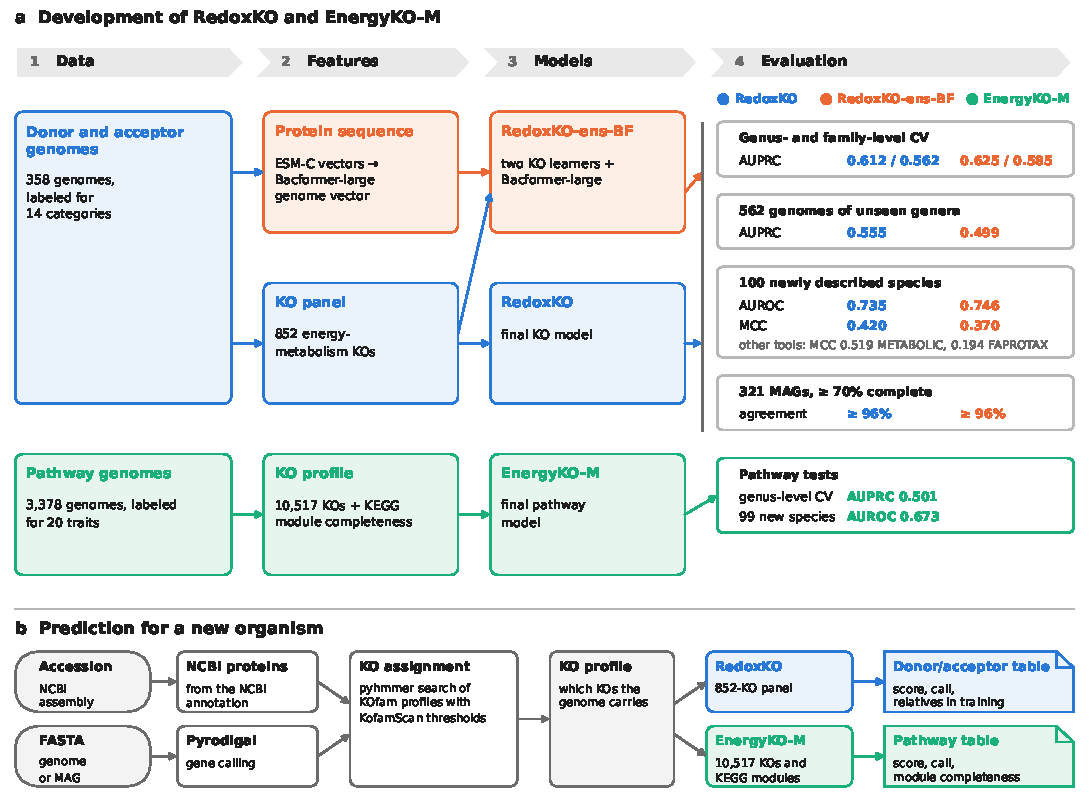
\includegraphics[width=1\linewidth,height=\textheight,keepaspectratio,alt={Study overview. (a) Model development. Colors mark the donor and acceptor task (blue), the pathway task (green) and the model with the Bacformer genome vector (orange). (b) Applying the final models to a new organism.}]{figures/Fig1_workflow.pdf}
\caption{\textbf{Study overview.} (a) Model development. Colors mark the
donor and acceptor task (blue), the pathway task (green) and the model
with the Bacformer genome vector (orange). (b) Applying the final models
to a new organism.}\label{fig:workflow}
\end{figure}

\subsection{RDF representation and access through
TogoMCP}\label{rdf-representation-and-access-through-togomcp}

We converted genome-protein-KO associations to Resource Description
Framework (RDF), representing assemblies, proteins, and KOs with
identifiers.org URIs. The graph retains individual protein assignments
as well as assignment-level attributes. This allows retrieval of either
a compact KO set for an assembly or the proteins and scores supporting a
specific annotated function.

The KofamScan definition file was also converted to RDF. KO descriptions
were represented with skos:definition, while profile metadata included
score thresholds and score types. Because definitions and assignments
use shared KO identifiers, queries can join the observed genomic
evidence to a description of its function. An assistant can consequently
request relevant subsets of annotations and their definitions instead of
receiving an entire proteome annotation table in its prompt.

The RDF data were loaded into QLever and made queryable through SPARQL.
Registering the dataset with TogoMCP enabled AI assistants to retrieve
these annotations alongside other resources available through RDF Portal
\autocite{Kinjo2026}, \autocite{Kawashima2018}. The implemented
integration supplies evidence for questions about the donors and
acceptors used by a specified organism. It exposes the annotation
resource; deployment of the trained trait classifier as a dedicated MCP
prediction tool is a separate step.

\subsection{Literature-assisted phenotype
collection}\label{literature-assisted-phenotype-collection}

Workflows assisted by large language models (LLMs) extracted electron
donor and acceptor information from research articles and microbial
databases, including BacDive \autocite{Schober2025}. One of these
workflows used FEDOT.MAS \autocite{FedotMAS2026}, which generates
multi-agent LLM pipelines from a task description. A meta-agent
(DeepSeek V4 Pro) generated the pipelines, and executor agents (Gemini
3.7 Flash) extracted donors and acceptors for 421 organisms from
open-access texts (PubMed, PubMed Central, Unpaywall and Europe PMC),
returning each value with a quoted string. We merged complementary
searches and extraction efforts, keeping supporting text, evidence
grades and conflicting claims. Database fields on nutrition, metabolite
utilization and oxygen tolerance supplied further context. These fields
need biological interpretation, because oxygen tolerance, for example,
differs from evidence of respiratory oxygen use.

The merged collection used four evidence grades. Grade A marked
statements of experimental evidence found by at least two extraction
efforts, and grade B marked such statements found by one effort. Grade C
covered genomic inference, hedged or review-only statements, weak
evidence and conflicting claims. Grade D covered unsupported, poorly
documented or disputed records. Agreement between extraction efforts
does not establish independent experimental replication, and the grades
do not imply that every record received expert review.

A snapshot of 16 September 2026 contained 1,817 evidence records, of
which 702 were grade A, 921 grade B, 136 grade C and 58 grade D. These
are statements, not distinct organisms or independent training examples.
The benchmark labels comprised 14 categories, seven for donors and seven
for acceptors. Some categories combined related physiology, such as
methanogenesis and acetogenesis, and residual categories grouped other
donors or acceptors. The evidence collection and the benchmark label
matrix therefore represent different levels of aggregation.

In October 2026 we audited the merged collection. Deterministic tools
checked that each cited source existed and contained its quote, and a
FEDOT.MAS pipeline (Gemini 3.8 Flash as executor) judged the remaining
flagged items. We applied a correction only when two independent runs
called an item an error and the corrected quote appeared exactly in its
source. Most errors concerned the supporting evidence, and fewer the
value itself (Supplementary Table \ref{tab:s_audit}). After the audit,
2.1\% of sampled values had a major error, a wrong value, organism or
role. This rate is similar to that of human and LLM-assisted data
extraction in systematic reviews \autocite{Gartlehner2025}.

\subsection{Marker references and comparative
visualization}\label{marker-references-and-comparative-visualization}

We assembled reference tables linking donor and acceptor transformations
to relevant genes, enzymes, and KO identifiers. A matching tool compared
these markers with genome annotations, and a web viewer displayed
genomic markers alongside reported substrates and evidence grades. The
viewer was developed for the broad RefSeq resource and the focused
autotroph collection.

Additional comparative displays used Jaccard similarity between KO sets
to organize genomes by their functional profiles. Such a representation
supports exploration of shared annotated capabilities; it should not be
interpreted as a sequence-based phylogeny. Together, the interfaces help
identify organisms for which literature-derived physiology and expected
genomic markers agree, and cases requiring closer examination. Some
phenotype entries and associated descriptive annotations remained
preliminary at the hackathon cutoff.

\subsection{Donor and acceptor
classifiers}\label{donor-and-acceptor-classifiers}

Training labels came from the phenotype collection. Each of the 358
labeled genomes has a yes/no label for 14 categories. Seven are electron
donors (sulfur compounds, ammonia, nitrite, H\textsubscript{2}, CO,
Fe(II) and other donors). The other seven are electron acceptors
(O\textsubscript{2}, nitrate by denitrification or DNRA, sulfate, sulfur
compounds, CO\textsubscript{2} by methanogenesis or acetogenesis,
Fe(III) and other acceptors). Other donors and other acceptors collect
all compounds outside the named categories. A genome is positive for a
category when the collection records at least one donor or acceptor of
that category for the organism, and negative otherwise, so a trait that
was never reported counts as absent. The 228 genomes of the focused
collection without any record are unlabeled. As a second, independent
source of labels we used a published trait compilation
\autocite{Madin2020}, which merges phenotype data for bacterial and
archaeal species from many published sources and which we call the
larger dataset. The category labels were assigned by the curators of the
collection in the shared genome table of 17 September 2026. They do not
record the evidence grade of the underlying statement, so a positive may
rest on genome-based inference as well as on a growth experiment.

We represented each genome by the presence or absence of 852 KOs. This
panel comprises every KO under KEGG BRITE Energy metabolism (09102) and
84 curated marker KOs, that is, genes chosen from the literature as
known markers of each category. We fixed this panel before fitting any
model. We did not use labels from the larger dataset for training, for
three reasons. First, we used part of it as our external test set, which
must stay separate from training. Second, it covers only 9 of our 14
categories. Third, its labels for lithotrophic donors are mostly
predicted by FAPROTAX \autocite{Louca2016} from taxonomy, whereas ours
come from the literature. To check this decision, we added its genomes,
with their labels, to training (Supplementary Table
\ref{tab:s_registered}), which lowered the ranking of nitrate tests on
new species (Discussion).

For each category, we trained a random forest \autocite{Breiman2001} of
500 trees, averaged over three random seeds, and chose its minimum leaf
size by inner cross-validation grouped by taxonomy. We refer to this
classifier as RedoxKO. We also trained L2-regularized logistic
regression and gradient-boosted trees (XGBoost) \autocite{Chen2016} on
the same KO features. RedoxKO-LX (L for logistic regression, X for
XGBoost) used the better of the two for each category, chosen by inner
cross-validation, and RedoxKO-ens averaged their probabilities. Both are
separate from the random forest RedoxKO.

The categories are imbalanced (Supplementary Table
\ref{tab:s_datasets}). RedoxKO therefore weighted the classes by inverse
frequency within each bootstrap sample of the random forest. We also
tried undersampling of negatives, oversampling of positives and no
weighting, and none performed significantly better (Supplementary Table
\ref{tab:s_balance}).

We chose decision thresholds that maximized the Matthews correlation
coefficient (MCC) \autocite{Matthews1975,Chicco2020} on inner
out-of-fold predictions, never on the test fold, and calibrated the
final scores with Platt scaling \autocite{Platt1999}. A category
received a yes/no call only if it met four conditions. First, in
family-level cross-validation, the lower bound of the 95\% confidence
interval of its MCC had to exceed 0.2. Second, in the same
cross-validation the model had to outperform the taxonomic baseline,
with a Benjamini-Hochberg (BH) adjusted q below 0.05. Third and fourth,
where the external genomes have labels for the category, its AUPRC on
them had to exceed the share of positive genomes, and the MCC of its
calls on these genomes had to exceed 0.2 as well. We added the fourth
condition on 22 October 2026, after all other results were known
(Supplementary Note 1). Supplementary Table \ref{tab:s_release} gives
these inputs for each category. The external genomes therefore took part
in deciding which categories get calls. Ammonia oxidation has no
external labels and no tests on new species, so its calls were checked
only in cross-validation. For categories that fail any of the
conditions, the workflow returns a score but no call.

\subsection{Sequence representations and
fusion}\label{sequence-representations-and-fusion}

We compared three ways to represent a genome by its protein sequences.
As a simple baseline used in earlier work \autocite{Hwang2024}, we
summarized protein embeddings from ESM-2 (35M parameters)
\autocite{Lin2023} and, in a separate model, from ESM-C (300M)
\autocite{EvolutionaryScale2024}. The summary was the average or the
maximum over all proteins of a genome, chosen by inner cross-validation.
We also weighted the ESM-2 embedding of each protein with
attention-based multiple-instance learning \autocite{Ilse2018}, and used
the genome vectors of Bacformer-base and Bacformer-large
\autocite{Wiatrak2025}. Bacformer reads ESM-C protein embeddings in
genomic order and, like other genome language models, represents each
protein in its genomic context \autocite{Hwang2024,Nguyen2024}. To
predict traits from the resulting genome vector, we compared logistic
regression with tree-based, tabular and neural learners and with
fine-tuning of Bacformer-large (Supplementary Table \ref{tab:s_dl}).
None did clearly better, so we kept logistic regression.

Combined models averaged the probabilities of a KO model and a sequence
model with equal weights. The strongest fusion, RedoxKO-ens-BF (BF for
Bacformer), combines RedoxKO-ens with the Bacformer-large classifier,
and RedoxKO-ens-ESM combines RedoxKO-ens with the ESM-2 model in the
same way. Taxonomy, organism names and literature were never inputs to
the supervised models.

\subsection{Pathway classifiers and module
completeness}\label{pathway-classifiers-and-module-completeness}

For pathway traits, we used every species in the larger dataset
\autocite{Madin2020} that has pathway labels and an annotated RefSeq
genome, one genome per species (Supplementary Table
\ref{tab:s_datasets}). The phenotype collection covers donors and
acceptors, and only part of its genomes have pathway labels. A pathway
model trained on these genomes alone could cover only a few of the 20
traits and was less accurate (Supplementary Table
\ref{tab:s_pathway174}). We therefore used the larger dataset, although
many of its labels, including most lithotrophic ones, are predicted by
FAPROTAX \autocite{Louca2016} from taxonomy. We merged its pathway terms
into traits and kept the 20 with at least 25 positive genomes. For these
genomes, and for the LLM prompts, we used the KofamScan annotations of
the shared resource, which agreed with our own annotation in 99.95\% of
genome-KO pairs on 306 genomes annotated both ways. Before fitting any
model, we split the genomes into five folds by genus and, separately, by
family.

We then compared three feature sets, the 852-KO panel, the full profile
of 10,517 KOs (EnergyKO), and the full profile plus the completeness of
KEGG energy modules (EnergyKO-M, M for modules). We also tested a
multi-label neural network, random forests \autocite{Breiman2001},
extra-trees \autocite{Geurts2006} and EnergyKO fused with
Bacformer-large (EnergyKO-BF). Each pathway model chose for each trait
between L2-regularized logistic regression and XGBoost by inner
cross-validation, as RedoxKO-LX does. We used the same baselines and
metrics as for donors and acceptors, and the first two conditions of the
release rule, because the pathway traits have no external test.
Following the registered rule, the final pathway model was the
registered model with the highest macro AUPRC in genus-level
cross-validation, EnergyKO-M. Extra-trees were added after this choice.

Separately, we scored the completeness of 71 KEGG modules covering
energy metabolism, carbon fixation, and methane, nitrogen and sulfur
metabolism \autocite{Kanehisa2025}. Each score is the share of a
module's steps covered by the genome's KOs. It is read directly from the
annotation.

\subsection{Cross-validation and evaluation
metrics}\label{cross-validation-and-evaluation-metrics}

We ran cross-validation at two levels, genus and family. At each level,
all genomes of a group stayed in the same fold, so no test genome had a
relative from its genus or family in training \autocite{Roberts2017}.
Many microbial traits are shared by close relatives, so a model can look
accurate because it recognizes relatives of the training genomes
\autocite{Goberna2016}. Grouping by genus or family removes this
shortcut. The pretrained sequence models, however, may still have seen
test genomes. We compared each model with three baselines. Curated
marker rules call a trait from its known genes. A frequency baseline
gives every genome the trait's overall frequency. A taxonomic baseline
gives each test genome the share of positive training genomes in the
lowest taxonomic rank that has training genomes, for example the family
in genus-level cross-validation, or the overall share where no relative
exists. A random split, used only for comparison, assigns genomes to
folds without regard to taxonomy. We never used test folds, external
genomes or newly described species for feature selection, hyperparameter
tuning or the decision thresholds of a model. The external genomes and
the newly described species did, however, take part in choosing between
the compared models, and the external genomes, through the release rule,
in deciding which categories get yes/no calls (Supplementary Note 1). We
also compared RedoxKO with a nearest-neighbor rule that gives each test
genome the similarity-weighted share of positives among the five
training genomes with the most similar KO content (Jaccard similarity on
the 852 KOs). This rule measures how much of the accuracy comes from
recognizing genomes with similar gene content alone.

The primary metric was the area under the precision-recall curve
(AUPRC), which remains informative when positives are rare
\autocite{Saito2015}. We computed it for each category on the
out-of-fold predictions of all five folds together and averaged it over
the 14 categories with equal weight, which we call macro AUPRC. We
summarized yes/no calls by the MCC. Because the MCC depends on how each
model's threshold was estimated, we ranked models by AUPRC. On the newly
described species, where most tests are positive, we summarized ranking
by the area under the receiver operating characteristic curve (AUROC).
We obtained 95\% confidence intervals by resampling whole genera or
families. We compared models by paired cluster-bootstrap intervals of
their difference and call two models tied when this interval includes
zero. Per-category tests against the taxonomic baseline use BH
correction within each group of tests.

External evaluation used 562 genomes from genera absent from training,
labeled from the larger dataset \autocite{Madin2020}. This set tests
transfer to new genera and to a second annotation source, although the
two sources may draw on overlapping publications. Its macro AUPRC covers
the nine categories that map onto the larger dataset, and we sampled the
set to contain positives for each. The larger dataset also supplies the
pathway labels, so the set is an external test for the donor and
acceptor models only.

Following recommendations for validating supervised learning in biology
\autocite{Walsh2021}, we recorded the models to compare, the splits, the
metrics and the release rule before scoring the first model. Later
experiments were registered in the same way before they were run
(Supplementary Table \ref{tab:s_registered}). The exceptions were the
rule for choosing the 100 new species of the main test, the extra-trees
pathway model and the analyses added last, such as the nearest-neighbor
rule. We recorded every change to the registered protocol with its date
and report the main changes in Supplementary Note 1. The most important
change, made after an internal audit, allowed a variant to replace the
final model only if its macro AUPRC was higher in cross-validation and
not lower on the external genomes. The random forest replaced the first
final model, RedoxKO-LX, after all other analyses had been done. Its
gain in cross-validation was not significant, so the switch rested on
the external genomes and on the calls on new species (Supplementary Note
1). Figure \ref{fig:workflow} summarizes the data, models and
evaluations.

\subsection{Feature attribution}\label{feature-attribution}

Within each outer genus-level fold, we fitted RedoxKO on the KO features
and computed TreeSHAP values \autocite{Lundberg2020} on the test genomes
of that fold. We called a KO stable if it ranked among the ten most
important in at least three of the five folds. We tested whether curated
marker KOs were enriched among stable features with a hypergeometric
test against all KOs in the feature set, with BH correction across
traits. To check that an association was not driven by phylum, we
re-tested it with a Cochran-Mantel-Haenszel test stratified by phylum
and by genome size, in five classes of KO count, because larger genomes
carry more KOs. Fisher's exact test then compared how often curated
markers and other genes passed this check.

Finally, we compared decision trees of depth three or less and
single-marker rules with RedoxKO by MCC on the same folds, with
genus-cluster bootstrap intervals.

\subsection{Newly described species}\label{newly-described-species}

To test the models against growth experiments, we searched PubMed for
species descriptions published from 2015 to 2026 that mention electron
donors or acceptors. We excluded every species whose genus, species or
genome occurred in the training, external or pathway data, and kept the
167 species with an annotated RefSeq genome and at least one reported
growth experiment. For 143 of them, six independent LLM agents extracted
each growth experiment, which we call a test, from the description paper
with its source and a quoted string, without access to gene content or
model output. A sheet for a human check of 50 extracted tests is
released, but this check has not yet been done. The other 24 species
came from an earlier hand-curated round without quoted strings, and
model output already existed for some of them, so we excluded them. An
audit then removed 12 extracted tests that were not real growth
experiments, such as reports of stimulated growth or of reduction during
fermentation. The primary set has 255 tests (number per category in Fig.
\ref{fig:percat}a).

We registered the scoring protocol before prediction. After the models
had scored the 143 species, we selected a primary set of 100 species,
one per genus. The selection used only the test labels and favored
species with tests in rare categories. It did not use the model scores.
We wrote this selection rule after scoring and did not register it. We
withheld the remaining 43 species from all later comparisons and used
them only to test choices made on the primary set. For a registered test
on autotroph-like species, we added further autotroph-like species from
description papers of 2000-2026 to those among the scored new species,
extracted in the same way (Supplementary Table \ref{tab:s_datasets}).
Confidence intervals come from bootstrapping description papers, because
species described together are not independent. By the same procedure,
we defined in advance a pathway set of all eligible species, one per
genus.

After choosing the final model, we froze it and ran two further blind
tests, each registered before any species was searched (Supplementary
Note 1). We searched PubMed again and excluded every genus, species and
genome of all earlier sets. The first test used species described in
2026. The second used description papers of lithotrophs from any year,
to obtain tests of electron donors. Because only eight such species came
from genera absent from all project data, the second test also included
species from genera absent from the training genomes, the same distance
to training as the external genomes. Tests were extracted, checked
against the source text and frozen before scoring, as for the primary
set.

\subsection{Comparison with other
tools}\label{comparison-with-other-tools}

We scored the same growth experiments with the following tools and
baselines.

\begin{itemize}
\tightlist
\item
  FAPROTAX 1.2.12 \autocite{Louca2016}, applied to the NCBI taxonomy of
  each species.
\item
  The taxonomic baseline, which gives each genome the label frequency of
  its relatives in training.
\item
  A rule based on curated marker KOs.
\item
  METABOLIC-G v4 \autocite{Zhou2022}.
\item
  The distillation step of DRAM on KOfam annotations
  \autocite{Shaffer2020}.
\item
  The machine-learning predictor of Microbe Decoder, queried through its
  public interface with KO content only \autocite{Hackmann2026}.
\item
  For oxygen use only, the BacDive aerobic model on InterProScan Pfam
  annotations \autocite{Koblitz2025,Jones2014}.
\end{itemize}

We mapped each tool's output to our categories by a rule fixed before
running the tool (Supplementary Table \ref{tab:s_mapping} for
METABOLIC). We scored categories that a tool does not cover as negative.
For calls on new species we pooled the MCC over all tests, because
several categories have fewer than ten tests, whereas on the external
genomes we averaged it over categories. We did not run Traitar
\autocite{Weimann2016}, whose phenotypes include no lithotrophic
electron donors, or gapseq \autocite{Zimmermann2021}, whose pathway
predictions would need a separate mapping onto our categories. All tools
that use KOfam annotations received the same KOfam release as our
models.

To compare RedoxKO with METABOLIC on more genomes, we reimplemented
METABOLIC's HMM searches with pyhmmer. The reimplementation reproduced
all of METABOLIC's category calls on the new species, and we applied it
to the external genomes and the MAG-isolate pairs. We also tested three
practical uses, the precision among the 20 top-ranked genomes per
category, the net benefit across decision thresholds in a decision curve
\autocite{Vickers2006}, and the accuracy of calls with a confident
label. Finally, we combined both tools in a per-category logistic
regression on RedoxKO's score and METABOLIC's call, fitted on the
training genomes only. We registered all these analyses in advance
(Supplementary Table \ref{tab:s_registered}).

\subsection{Confidence labels}\label{confidence-labels}

A user acting on a single genome needs to know which calls to trust. We
therefore converted the scores of RedoxKO into class-conditional
(Mondrian) conformal prediction sets \autocite{Angelopoulos2023}, which
we report as confidence labels. We calibrated the sets on scores that
the training genomes received in family-level cross-validation. Each
prediction is then labeled a confident yes, a confident no or uncertain,
and in rare cases receives no label. The sets are built to contain the
correct answer for at least 90\% of genomes that resemble the
calibration genomes. Test genomes come from new genera, so coverage on
them can fall below this target. The released workflow adds these labels
to the predictions of RedoxKO in the six categories that get yes/no
calls.

\subsection{Metagenome-assembled genomes and
habitats}\label{metagenome-assembled-genomes-and-habitats}

From GTDB release 232 \autocite{Parks2022} we paired MAGs with isolate
genomes of the same species from the external and new-species sets. All
MAGs had a completeness of at least 50\% and a contamination of at most
10\%, as estimated with CheckM2 \autocite{Chklovski2023}. We chose one
MAG per species at random in each completeness bin (50-70\%, 70-90\% and
at least 90\%). We predicted both genomes of a pair from nucleotide
sequence with the same gene caller. For a case study on uncultured
organisms, we selected 300 high-quality MAGs (at least 90\% complete and
at most 5\% contaminated), at most one per genus. We assigned each MAG
to one of five habitats (hydrothermal vents, acid mine drainage,
anaerobic digesters, seawater and the human gut) by matching its
isolation source against keywords chosen before the analysis. We tested
five expectations about their predicted capabilities that we had
recorded before the analysis, each comparing the habitat expected to be
higher with one or more other habitats, in nine tests in total. We used
a one-sided Fisher's exact test on the yes/no calls, or a one-sided
Mann-Whitney test on the scores for Fe(II) and H\textsubscript{2}
oxidation, which have no calls. We corrected all nine p values together
with the BH method.

\subsection{Comparison with large language
models}\label{comparison-with-large-language-models}

We compared two large language models (LLMs) with the trained models on
96 labeled genomes. Before querying any model, we selected these genomes
as a stratified random sample with a fixed seed that kept at least five
positives per category where possible. For each genome, the prompt
listed which panel KOs KofamScan had assigned, taken from the shared RDF
resource. Each KO came with its identifier and its KEGG definition, for
example K00370 with ``nitrate reductase / nitrite oxidoreductase, alpha
subunit'', together with the number of matching proteins and the best
ratio of score to threshold. The prompt asked for the probability that
the organism uses each category as defined in the database. We gave each
genome two prompts. In the anonymized prompt, a code replaced the
organism name, and the named prompt also gave the name. Neither prompt
gave the taxonomy of the organism. Comparing the two prompts shows
whether a model reads the supplied gene evidence or relies on knowledge
about the organism.

We ran Claude Opus 5 (claude-opus-5) on 17 and 20 September 2026 as
isolated agents in Claude Code that read only the input batch, and the
prompt forbade any tool, web search or outside lookup. These agents used
default sampling settings, which this interface does not expose, and
made one pass per genome. We queried GPT-6 Astra (openai/gpt-6-astra)
through OpenRouter on 17 September 2026 at temperature 0 with JSON
output, without tools or web search. The named GPT run stopped after 84
genomes when the API budget ran out and was not repeated, so its paired
comparisons use those 84 genomes. We then applied the same design to the
20 pathway traits with Claude Opus 5, using pathway definitions in place
of donor and acceptor categories. Prompts, inputs and raw outputs are in
the repository.

\subsection{Software and computing}\label{software-and-computing}

We computed protein embeddings on two NVIDIA T4 GPUs and ran all other
steps on a single Apple M3 Pro workstation (11 cores, 18 GB). KO
assignment with pyhmmer runs on CPU only. Supplementary Table
\ref{tab:s_models} gives the run time per genome of each released model.
Software versions and the KOfam release are pinned in the repository.

\section{Results}\label{results}

\subsection{A shared resource for genomic and physiological
evidence}\label{a-shared-resource-for-genomic-and-physiological-evidence}

The hackathon produced a searchable genome-protein-KO resource, an
assembly-linked phenotype collection, and interfaces connecting the two.
Through TogoMCP, an assistant could retrieve an organism's annotated
functions, inspect their definitions, and incorporate them into answers
about electron donors and acceptors. The viewer made these genomic
markers inspectable alongside reported physiology and evidence grades.
The resulting workflow connects what an organism has been reported to
use with what its genome encodes.

This evidence-retrieval capability and the prediction benchmark serve
distinct purposes. A named-organism answer can incorporate published
physiological observations and therefore cannot alone demonstrate
prediction accuracy for uncharacterized genomes. The supervised
benchmark addressed the latter question by withholding complete
taxonomic groups during evaluation.

\subsection{Gene content predicts donor and acceptor use in unseen
genera and
families}\label{gene-content-predicts-donor-and-acceptor-use-in-unseen-genera-and-families}

We first tested how well gene content predicts donor and acceptor use in
organisms whose genus or family was not seen in training. In genus-level
cross-validation, RedoxKO reached a macro AUPRC of 0.612, above the
taxonomic baseline and the curated marker rules, and it also exceeded
both in family-level cross-validation (Table \ref{tab:cv}). A model that
combines many genes therefore predicted the labels better than marker
rules or label transfer by taxonomy. A simpler rule that copies the
labels of the training genomes with the most similar KO content,
however, came close to RedoxKO in cross-validation, and the difference
between the two was not significant (Table \ref{tab:cv}). Much of the
accuracy in cross-validation can therefore be reached through similarity
in gene content alone. On the external genomes, whose labels come from a
second source, RedoxKO was clearly better than this rule. The lead of
RedoxKO also did not depend on positive labels that might have been
inferred from genes. When only positives backed by growth experiments
were kept, RedoxKO stayed as far ahead of the taxonomic baseline as
before (Supplementary Table \ref{tab:s_paired}). Accuracy declined as
test genomes became more distant from training. The macro AUPRC of
RedoxKO was highest with a random split, lower with genera held out and
lowest with families held out (Supplementary Table \ref{tab:s_splits}).
The higher score with a random split shows that close relatives in
training make the model look more accurate than it is for organisms
without such relatives.

Sequence representations did not clearly add to gene content (Table
\ref{tab:cv}). Bacformer-large alone scored below RedoxKO, and learning
a weight for each protein (attention-based MIL) did not improve on
averaging the protein embeddings. RedoxKO-ens-BF, which adds
Bacformer-large to the KO learners, scored higher than RedoxKO in every
fold allocation, but on the external genomes it scored lower. It was
also never significantly better than RedoxKO-ens, its own KO learners
(Supplementary Table \ref{tab:s_paired}). Whether a language model adds
anything beyond gene content would need more labeled genomes to show.

The lead of RedoxKO in genus-level cross-validation depended on how the
genera were split into folds. Averaged over the six fold allocations,
RedoxKO and RedoxKO-LX performed about equally, and RedoxKO was
significantly better in only one of them (Supplementary Tables
\ref{tab:s_splits} and \ref{tab:s_paired}).

\subsection{Accuracy depends on whether a trait has defined marker
genes}\label{accuracy-depends-on-whether-a-trait-has-defined-marker-genes}

Macro averages hid large differences among categories (Table
\ref{tab:pertrait}). Five categories, among them sulfate reduction,
sulfur oxidation and ammonia oxidation, reached AUPRC above 0.85,
whereas Fe(III) reduction, other donors and other acceptors scored low.
Prevalence alone did not explain these differences. Nitrite oxidation
had the fewest positives, yet its AUPRC was twenty times its prevalence
(Table \ref{tab:pertrait}). Fe(III) reduction, by contrast, reached only
0.22 at a prevalence of 9\%. The 852-KO panel lacks KOs for the MtrCAB
complex for extracellular electron transfer \autocite{Shi2016}, and
adding them through curated HMMs or multiheme cytochrome counts did not
improve the score. For common traits, a high AUPRC can go with a modest
MCC, so good calls also need a threshold chosen for each category.

\par

\penalty-100\begingroup\dimen0=32\baselineskip\dimen2=\pagegoal\advance\dimen2-\pagetotal\ifdim\dimen0>\dimen2\ifdim\dimen2>0pt\vfil\fi\penalty-10000\fi\endgroup

\begingroup\small\hyphenpenalty=10000\renewcommand{\arraystretch}{1.25}

\begin{longtable}[]{@{}
  >{\raggedright\arraybackslash}p{(\linewidth - 8\tabcolsep) * \real{0.3768}}
  >{\raggedright\arraybackslash}p{(\linewidth - 8\tabcolsep) * \real{0.2319}}
  >{\raggedleft\arraybackslash}p{(\linewidth - 8\tabcolsep) * \real{0.1159}}
  >{\raggedleft\arraybackslash}p{(\linewidth - 8\tabcolsep) * \real{0.1304}}
  >{\raggedleft\arraybackslash}p{(\linewidth - 8\tabcolsep) * \real{0.1449}}@{}}
\caption{\textbf{Performance of donor and acceptor models.} Macro AUPRC
in genus- and family-level cross-validation over 14 categories, and over
nine categories on the external genomes. Bold marks the best value per
column. Cross-validation uses the folds of this paper (other fold
allocations in Supplementary Table \ref{tab:s_splits}). RedoxKO was
chosen after the external test, so its external value is not blind.
\label{tab:cv}}\tabularnewline
\toprule\noalign{}
\begin{minipage}[b]{\linewidth}\raggedright
Model
\end{minipage} & \begin{minipage}[b]{\linewidth}\raggedright
Features
\end{minipage} & \begin{minipage}[b]{\linewidth}\raggedleft
Genus-level CV
\end{minipage} & \begin{minipage}[b]{\linewidth}\raggedleft
Family-level CV
\end{minipage} & \begin{minipage}[b]{\linewidth}\raggedleft
External genomes
\end{minipage} \\
\midrule\noalign{}
\endfirsthead
\toprule\noalign{}
\begin{minipage}[b]{\linewidth}\raggedright
Model
\end{minipage} & \begin{minipage}[b]{\linewidth}\raggedright
Features
\end{minipage} & \begin{minipage}[b]{\linewidth}\raggedleft
Genus-level CV
\end{minipage} & \begin{minipage}[b]{\linewidth}\raggedleft
Family-level CV
\end{minipage} & \begin{minipage}[b]{\linewidth}\raggedleft
External genomes
\end{minipage} \\
\midrule\noalign{}
\endhead
\bottomrule\noalign{}
\endlastfoot
\emph{Baselines} & & & & \\*
\quad Frequency baseline & none & 0.185 & 0.178 & 0.183 \\
\quad Curated marker rules & marker KOs & 0.317 & 0.317 & 0.338 \\
\quad Taxonomic baseline & taxonomy & 0.472 & 0.380 & 0.380 \\
\quad Nearest-neighbor rule & 852 KOs & 0.572 & 0.531 & 0.436 \\
\emph{Sequence models} & & & & \\*
\quad ESM-2 & ESM-2 & 0.544 & 0.497 & 0.421 \\
\quad Attention-based MIL & ESM-2 & 0.548 & 0.495 & 0.405 \\
\quad Bacformer-large & Bacformer & 0.577 & 0.531 & 0.440 \\
\emph{KO models} & & & & \\*
\quad RedoxKO & 852 KOs & 0.612 & 0.562 & \textbf{0.555} \\
\quad RedoxKO-LX & 852 KOs & 0.576 & 0.560 & 0.511 \\
\quad RedoxKO-ens & 852 KOs & 0.602 & 0.573 & 0.504 \\
\emph{Combined models} & & & & \\*
\quad RedoxKO-ens-ESM & KOs, ESM-2 & 0.616 & 0.584 & 0.483 \\
\quad RedoxKO-ens-BF & KOs, Bacformer & \textbf{0.625} & \textbf{0.585}
& 0.499 \\
\end{longtable}

\endgroup

\par

\penalty-100\begingroup\dimen0=27\baselineskip\dimen2=\pagegoal\advance\dimen2-\pagetotal\ifdim\dimen0>\dimen2\ifdim\dimen2>0pt\vfil\fi\penalty-10000\fi\endgroup

\begingroup\small\hyphenpenalty=10000\renewcommand{\arraystretch}{1.25}

\begin{longtable}[]{@{}
  >{\raggedright\arraybackslash}p{(\linewidth - 12\tabcolsep) * \real{0.2763}}
  >{\raggedright\arraybackslash}p{(\linewidth - 12\tabcolsep) * \real{0.1842}}
  >{\raggedleft\arraybackslash}p{(\linewidth - 12\tabcolsep) * \real{0.0921}}
  >{\raggedleft\arraybackslash}p{(\linewidth - 12\tabcolsep) * \real{0.1447}}
  >{\raggedleft\arraybackslash}p{(\linewidth - 12\tabcolsep) * \real{0.1184}}
  >{\raggedleft\arraybackslash}p{(\linewidth - 12\tabcolsep) * \real{0.0789}}
  >{\raggedright\arraybackslash}p{(\linewidth - 12\tabcolsep) * \real{0.1053}}@{}}
\caption{\textbf{Performance of RedoxKO by category.} AUPRC, taxonomic
baseline and MCC are from genus-level cross-validation. The release rule
uses family-level cross-validation (Supplementary Table
\ref{tab:s_release}). \label{tab:pertrait}}\tabularnewline
\toprule\noalign{}
\begin{minipage}[b]{\linewidth}\raggedright
Category
\end{minipage} & \begin{minipage}[b]{\linewidth}\raggedright
Positives (prevalence)
\end{minipage} & \begin{minipage}[b]{\linewidth}\raggedleft
AUPRC
\end{minipage} & \begin{minipage}[b]{\linewidth}\raggedleft
Taxonomic baseline
\end{minipage} & \begin{minipage}[b]{\linewidth}\raggedleft
AUPRC, family-level CV
\end{minipage} & \begin{minipage}[b]{\linewidth}\raggedleft
MCC
\end{minipage} & \begin{minipage}[b]{\linewidth}\raggedright
Output
\end{minipage} \\
\midrule\noalign{}
\endfirsthead
\toprule\noalign{}
\begin{minipage}[b]{\linewidth}\raggedright
Category
\end{minipage} & \begin{minipage}[b]{\linewidth}\raggedright
Positives (prevalence)
\end{minipage} & \begin{minipage}[b]{\linewidth}\raggedleft
AUPRC
\end{minipage} & \begin{minipage}[b]{\linewidth}\raggedleft
Taxonomic baseline
\end{minipage} & \begin{minipage}[b]{\linewidth}\raggedleft
AUPRC, family-level CV
\end{minipage} & \begin{minipage}[b]{\linewidth}\raggedleft
MCC
\end{minipage} & \begin{minipage}[b]{\linewidth}\raggedright
Output
\end{minipage} \\
\midrule\noalign{}
\endhead
\bottomrule\noalign{}
\endlastfoot
Sulfate reduction & 63 (18\%) & 0.915 & 0.835 & 0.878 & 0.80 & yes/no \\
Sulfur oxidation & 131 (37\%) & 0.896 & 0.708 & 0.860 & 0.69 & yes/no \\
H\textsubscript{2} oxidation & 208 (58\%) & 0.880 & 0.814 & 0.877 & 0.50
& score \\
Methanogen/acetogen & 75 (21\%) & 0.870 & 0.821 & 0.858 & 0.75 &
yes/no \\
Ammonia oxidation & 32 (9\%) & 0.869 & 0.653 & 0.700 & 0.74 & yes/no \\
O\textsubscript{2} respiration & 177 (49\%) & 0.798 & 0.770 & 0.764 &
0.76 & yes/no \\
Nitrate reduction & 102 (28\%) & 0.688 & 0.507 & 0.595 & 0.49 & score \\
Nitrite oxidation & 12 (3\%) & 0.672 & 0.050 & 0.553 & 0.38 & score \\
Sulfur reduction & 50 (14\%) & 0.584 & 0.399 & 0.622 & 0.36 & yes/no \\
CO oxidation & 45 (13\%) & 0.503 & 0.350 & 0.504 & 0.57 & score \\
Fe(II) oxidation & 43 (12\%) & 0.436 & 0.259 & 0.237 & 0.36 & score \\
Fe(III) reduction & 32 (9\%) & 0.223 & 0.184 & 0.135 & 0.10 & score \\
Other donors & 23 (6\%) & 0.135 & 0.081 & 0.161 & 0.19 & score \\
Other acceptors & 23 (6\%) & 0.104 & 0.180 & 0.120 & 0.04 & score \\
\end{longtable}

\endgroup

\subsection{Key features match known marker genes where KEGG has
them}\label{key-features-match-known-marker-genes-where-kegg-has-them}

To test whether the models detect metabolic genes or merely recognize
relatives, we computed TreeSHAP attributions on genera absent from
training, for RedoxKO and for random forests trained on the pathway
traits. Curated marker genes were significantly enriched among the
stable features in 4 of 14 donor and acceptor categories and in 9 of 20
pathway traits (Fig. \ref{fig:xai}a and Supplementary Fig.
\ref{fig:s_pathways}). The two iron categories could not show this
enrichment, because they have no marker among the KEGG features. The
stable features were mostly known pathway genes. For nitrate reduction
they included \emph{narJ}, \emph{narI}, \emph{norB}, \emph{napB} and,
below the top five, \emph{nosZ} (Fig. \ref{fig:xai}b). For sulfur
oxidation they included \emph{sox} genes and \emph{sqr}, and for ammonia
oxidation the ammonia monooxygenase subunits \emph{amoB} and \emph{amoC}
(not shown in Fig. \ref{fig:xai}b). For sulfate reduction, they also
included \emph{dsrM}, \emph{dsrK} and, below the top five, \emph{dsrO},
which were missing from our list of marker genes. These genes encode
subunits of the membrane complex DsrMKJOP, which reduces the DsrC
trisulfide formed by sulfite reductase \autocite{Santos2015}.

Two kinds of category behaved differently. The model predicted oxygen
respiration mainly from the absence of genes typical of methanogens and
other strict anaerobes (\emph{hdrA2}, \emph{hdrB2}, \emph{mvhD},
\emph{cdhE}), and less from genes of terminal oxidases. It therefore
relies on a correlate of aerobic respiration. Oxygen use can also be
predicted from genome features without functional annotation
\autocite{Flamholz2024}, and such predictions support analyses of oxygen
adaptation across bacteria \autocite{Davin2025}. Our attributions
suggest why these approaches work even without relying on oxidase genes.
Iron oxidation and reduction, like the manganese, arsenate and fumarate
pathways, have no KO in our list of curated markers, consistent with
their low accuracy (Table \ref{tab:pertrait} and Supplementary Table
\ref{tab:s_pathway_traits}).

Most of these associations did not hold within phyla. Only 15 of the 59
stable features stayed associated with their trait after controlling for
phylum and genome size. Curated markers held up significantly more often
than other genes (10 of 17 against 5 of 42). The associations that
survive phylum control therefore mostly reflect known biology. The
others may reflect shared ancestry, or too few genomes per phylum to
test them.

Comparison with simple rules showed where learning adds accuracy (Fig.
\ref{fig:xai}c). For ammonia oxidation, nitrate reduction and
methanogenesis and acetogenesis, a single-marker rule (\emph{amoB},
\emph{narG} or \emph{napA}, or a methanogenesis or acetogenesis marker)
matched or exceeded RedoxKO on genera absent from training. Where no
single gene defines the trait, the model was better, most clearly for
hydrogen oxidation against a hydrogenase rule and for oxygen respiration
against a terminal-oxidase rule, and also for sulfate reduction against
\emph{dsrB} alone. Decision trees of depth three or less matched RedoxKO
in the categories with clear marker genes, but were significantly worse
for oxygen respiration and sulfur reduction.

\begin{figure}
\centering
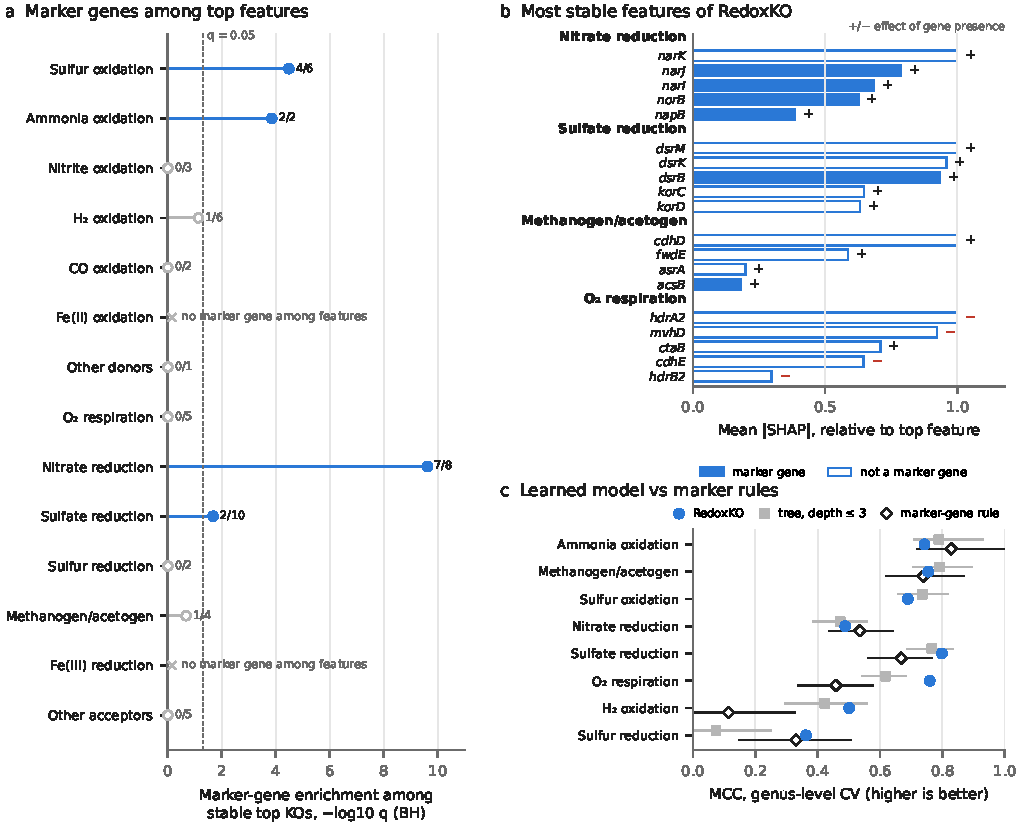
\includegraphics[width=1\linewidth,height=\textheight,keepaspectratio,alt={Top features and their agreement with known markers. (a) Marker genes among the most stable features of RedoxKO (for example 4/6). Grey points are not significant. (b) Most stable features. (c) MCC of RedoxKO, trees of depth three or less and single-marker rules, with 95\% genus-bootstrap intervals of the difference from RedoxKO. Sulfur oxidation has no single-marker rule.}]{figures/Fig_xai.pdf}
\caption{\textbf{Top features and their agreement with known markers.}
(a) Marker genes among the most stable features of RedoxKO (for example
4/6). Grey points are not significant. (b) Most stable features. (c) MCC
of RedoxKO, trees of depth three or less and single-marker rules, with
95\% genus-bootstrap intervals of the difference from RedoxKO. Sulfur
oxidation has no single-marker rule.}\label{fig:xai}
\end{figure}

\subsection{Predictions transfer to unseen genera of the larger
dataset}\label{predictions-transfer-to-unseen-genera-of-the-larger-dataset}

We next tested whether the models transfer beyond the training data. On
the external genomes, RedoxKO again clearly outperformed the taxonomic
baseline (Table \ref{tab:cv}), also on a subset with balanced category
sizes. The training genomes were chosen as autotrophs, but only about
half of the external genomes and new species carry a carbon-fixation or
methanogenesis module that is at least 80\% complete (Supplementary
Table \ref{tab:s_autotroph}). RedoxKO ranked the other genomes about as
well, and on newly described autotroph-like species it ranked growth
experiments at least as well as on all new species (Supplementary Table
\ref{tab:s_autotroph}). This result depends, however, on how categories
and missing values were matched between the two datasets. For the
species in both datasets, the two label sources agreed moderately,
mainly because they differ for hydrogen oxidation (Supplementary Note
3).

On the external genomes, RedoxKO scored highest (Table \ref{tab:cv}),
also above RedoxKO-LX (Supplementary Table \ref{tab:s_paired}), and the
margin over RedoxKO-LX was the same for genomes whose labels do not come
from FAPROTAX. RedoxKO-ens and RedoxKO-ens-BF, which had scored as high
in cross-validation, did not keep this level on the external genomes.
Because RedoxKO scored higher on the external genomes and gave more
accurate calls on new species, it became the final model in place of
RedoxKO-LX, although the two were tied in cross-validation
(Supplementary Note 1). It runs on a CPU, and because each of its
features is a gene, every prediction can be traced to genes (Fig.
\ref{fig:xai}).

RedoxKO-ens-BF ranked the growth experiments of newly described species
about as well as RedoxKO. It ranked the external genomes less well and
needs protein embeddings computed on a GPU, so we release it only as an
alternative for users who already have Bacformer-large vectors.

\subsection{Models rank growth experiments of new species moderately
well}\label{models-rank-growth-experiments-of-new-species-moderately-well}

Cross-validation removes close relatives from training but reuses the
label source of the training data. We therefore tested the models
against published growth experiments on newly described species, each
from a genus absent from all project data. RedoxKO and RedoxKO-ens-BF
ranked these tests with similar AUROC (Table \ref{tab:newspecies}). On
all 143 scored species, RedoxKO reached an AUROC of 0.73, and 0.76
without the three categories with fewer than ten tests.

Accuracy and MCC are poor guides on this test set, because most tests
are positive and the share differs between categories. A rule that gives
each category its most common outcome in this test set (test-set
majority) reached a higher accuracy and MCC than any model (Table
\ref{tab:newspecies}). This rule uses the test labels, so no one could
apply it to a new genome. We therefore compare models mainly by AUROC,
which does not depend on a threshold or on the share of positive tests.
Bacformer-large had the highest MCC among the models but a lower AUROC
than the KO-based models. Its yes/no calls benefited from a threshold
that happened to suit the many positive tests in this set, whereas its
ranking, which does not depend on a threshold, was weaker. We therefore
kept the KO-based models, which ranked tests better and whose
predictions can be traced to genes.

The calls were conservative. Positive calls of RedoxKO were mostly
correct (86\%), whereas negative calls were often wrong (56\% correct).
Errors were concentrated in a few categories, above all iron reduction
(Fig. \ref{fig:percat}a). RedoxKO returns only a score for this
category, so these errors would not be issued as yes/no calls. Hydrogen
oxidation passed the first three conditions of the release rule, but its
calls were poor on the external genomes and on new species (Fig.
\ref{fig:percat}), and on the external genomes RedoxKO called most
negative genomes positive. It failed the fourth condition, which we
added after all other results were known, so the workflow returns only a
score for it. When only the six categories in which RedoxKO gives calls
were counted (five of them have tests), 72\% of its calls were correct.
Its MCC was slightly lower than that of METABOLIC and DRAM, but neither
difference was significant (Supplementary Table \ref{tab:s_paired}).

\par

\penalty-100\begingroup\dimen0=22\baselineskip\dimen2=\pagegoal\advance\dimen2-\pagetotal\ifdim\dimen0>\dimen2\ifdim\dimen2>0pt\vfil\fi\penalty-10000\fi\endgroup

\begingroup\small\hyphenpenalty=10000\renewcommand{\arraystretch}{1.25}

\begin{longtable}[]{@{}
  >{\raggedright\arraybackslash}p{(\linewidth - 10\tabcolsep) * \real{0.3421}}
  >{\raggedleft\arraybackslash}p{(\linewidth - 10\tabcolsep) * \real{0.0921}}
  >{\raggedleft\arraybackslash}p{(\linewidth - 10\tabcolsep) * \real{0.1316}}
  >{\raggedleft\arraybackslash}p{(\linewidth - 10\tabcolsep) * \real{0.0921}}
  >{\raggedleft\arraybackslash}p{(\linewidth - 10\tabcolsep) * \real{0.1711}}
  >{\raggedleft\arraybackslash}p{(\linewidth - 10\tabcolsep) * \real{0.1711}}@{}}
\caption{\textbf{Tests on new species.} Performance on 255 growth
experiments of 100 new species. AUROC is averaged over categories. The
reference rules give one fixed answer per category. Training frequency
calls a category present when at least half of the training genomes have
it. Bold marks the best model per column.
\label{tab:newspecies}}\tabularnewline
\toprule\noalign{}
\begin{minipage}[b]{\linewidth}\raggedright
Model
\end{minipage} & \begin{minipage}[b]{\linewidth}\raggedleft
AUROC
\end{minipage} & \begin{minipage}[b]{\linewidth}\raggedleft
Accuracy
\end{minipage} & \begin{minipage}[b]{\linewidth}\raggedleft
MCC
\end{minipage} & \begin{minipage}[b]{\linewidth}\raggedleft
Sensitivity
\end{minipage} & \begin{minipage}[b]{\linewidth}\raggedleft
Specificity
\end{minipage} \\
\midrule\noalign{}
\endfirsthead
\toprule\noalign{}
\begin{minipage}[b]{\linewidth}\raggedright
Model
\end{minipage} & \begin{minipage}[b]{\linewidth}\raggedleft
AUROC
\end{minipage} & \begin{minipage}[b]{\linewidth}\raggedleft
Accuracy
\end{minipage} & \begin{minipage}[b]{\linewidth}\raggedleft
MCC
\end{minipage} & \begin{minipage}[b]{\linewidth}\raggedleft
Sensitivity
\end{minipage} & \begin{minipage}[b]{\linewidth}\raggedleft
Specificity
\end{minipage} \\
\midrule\noalign{}
\endhead
\bottomrule\noalign{}
\endlastfoot
RedoxKO-ens-BF & \textbf{0.746} & 66.3\% & 0.370 & 56.9\% & 80.4\% \\
RedoxKO & 0.735 & 67.8\% & 0.420 & 55.6\% & 86.3\% \\
RedoxKO-LX & 0.732 & 64.7\% & 0.364 & 51.6\% & 84.3\% \\
RedoxKO-ens & 0.705 & 64.3\% & 0.374 & 49.0\% & \textbf{87.3\%} \\
Bacformer-large alone & 0.679 & \textbf{69.4\%} & \textbf{0.444} &
\textbf{58.2\%} & 86.3\% \\
ESM-C alone & 0.667 & 63.1\% & 0.290 & 56.9\% & 72.5\% \\
\emph{Reference rules} & & & & & \\*
\quad Training frequency & 0.500 & 45.1\% & 0.128 & 11.1\% & 96.1\% \\
\quad Test-set majority & 0.500 & 74.1\% & 0.451 & 83.0\% & 60.8\% \\
\end{longtable}

\endgroup

\subsection{Comparison with existing
tools}\label{comparison-with-existing-tools}

We scored seven tools and baselines on the same 255 growth experiments
(Table \ref{tab:tools}). The models outperformed taxonomy-based tools,
which depend on close references \autocite{Goberna2016,Douglas2020}.
FAPROTAX, for example, recognized only about a quarter of the species,
and even on those its calls were less accurate than those of RedoxKO.
The rule-based tools did at least as well as RedoxKO. METABOLIC gave the
most accurate yes/no calls when all tests were pooled and DRAM when
accuracy was averaged over categories, but none of these differences was
significant. The same held in the categories in which RedoxKO gives
calls, where no single category differed significantly (Fig.
\ref{fig:percat}a). METABOLIC was ahead mainly in sulfur reduction, and
also in hydrogen oxidation, for which RedoxKO returns only a score.

On the 43 withheld species, the only set that played no part in choosing
the final model, the picture was similar. METABOLIC again had the more
accurate pooled calls and RedoxKO the more accurate calls averaged over
categories, and neither difference was significant. RedoxKO ranked these
tests less well than those of the primary set, which may be chance in
this small set (Table \ref{tab:tools}).

Two blind tests, run after the final model was frozen, gave a similar
picture (Supplementary Table \ref{tab:s_blind}). RedoxKO ranked the
tests of new lithotrophic species about as well as those of the primary
set. Its ranking of electron donors was uncertain, because the
description papers reported few negative donor tests. Hydrogen and
sulfur oxidation were ranked well, but carbon monoxide oxidation, with
only one negative test, was not. Species described in 2026 gave tests
almost only for oxygen respiration, which RedoxKO ranked well. On the
lithotrophic species, RedoxKO-LX ranked the tests about as well and made
slightly more accurate calls, whereas on the withheld species RedoxKO
ranked the tests better. The sets that played no part in choosing the
final model therefore show no consistent advantage of either model.

Of the other learned predictors, Microbe Decoder made less accurate
calls than RedoxKO on its three categories and ranked the tests less
well, and the BacDive aerobic model ranked oxygen tests as well as
RedoxKO.

RedoxKO's scores were also useful alongside METABOLIC's calls. Among the
tests that METABOLIC called positive, RedoxKO's scores separated the
true from the false positives. We first saw this on the 100 species and
then confirmed it on the 43 withheld species, in a test registered with
RedoxKO-LX and repeated with RedoxKO. Ranking tests by METABOLIC's call
and then by RedoxKO's score worked better than METABOLIC alone, but not
better than RedoxKO alone (Supplementary Table \ref{tab:s_registered}).

\par

\penalty-100\begingroup\dimen0=32\baselineskip\dimen2=\pagegoal\advance\dimen2-\pagetotal\ifdim\dimen0>\dimen2\ifdim\dimen2>0pt\vfil\fi\penalty-10000\fi\endgroup

\begingroup\small\hyphenpenalty=10000\renewcommand{\arraystretch}{1.25}

\begin{longtable}[]{@{}
  >{\raggedright\arraybackslash}p{(\linewidth - 10\tabcolsep) * \real{0.2604}}
  >{\raggedright\arraybackslash}p{(\linewidth - 10\tabcolsep) * \real{0.1667}}
  >{\raggedleft\arraybackslash}p{(\linewidth - 10\tabcolsep) * \real{0.0729}}
  >{\raggedleft\arraybackslash}p{(\linewidth - 10\tabcolsep) * \real{0.1042}}
  >{\raggedleft\arraybackslash}p{(\linewidth - 10\tabcolsep) * \real{0.0729}}
  >{\raggedright\arraybackslash}p{(\linewidth - 10\tabcolsep) * \real{0.3229}}@{}}
\caption{\textbf{Comparison with other tools.} 255 growth experiments of
100 new species and, in the last group, 75 of the 43 withheld species.
MCC is pooled over tests or averaged over categories, uncovered ones
counted as negative. Dashes mark values not computed, because a tool
gives only yes/no calls or covers too few categories. Notes give
METABOLIC minus RedoxKO in MCC (Supplementary Table \ref{tab:s_paired}).
Bold marks the best primary value per column among tools scored on all
tests. \label{tab:tools}}\tabularnewline
\toprule\noalign{}
\begin{minipage}[b]{\linewidth}\raggedright
Tool
\end{minipage} & \begin{minipage}[b]{\linewidth}\raggedright
Input
\end{minipage} & \begin{minipage}[b]{\linewidth}\raggedleft
MCC
\end{minipage} & \begin{minipage}[b]{\linewidth}\raggedleft
MCC, category mean
\end{minipage} & \begin{minipage}[b]{\linewidth}\raggedleft
AUROC
\end{minipage} & \begin{minipage}[b]{\linewidth}\raggedright
Note
\end{minipage} \\
\midrule\noalign{}
\endfirsthead
\toprule\noalign{}
\begin{minipage}[b]{\linewidth}\raggedright
Tool
\end{minipage} & \begin{minipage}[b]{\linewidth}\raggedright
Input
\end{minipage} & \begin{minipage}[b]{\linewidth}\raggedleft
MCC
\end{minipage} & \begin{minipage}[b]{\linewidth}\raggedleft
MCC, category mean
\end{minipage} & \begin{minipage}[b]{\linewidth}\raggedleft
AUROC
\end{minipage} & \begin{minipage}[b]{\linewidth}\raggedright
Note
\end{minipage} \\
\midrule\noalign{}
\endhead
\bottomrule\noalign{}
\endlastfoot
\emph{Learned models} & & & & & \\*
\quad RedoxKO & KOs & 0.420 & 0.290 & 0.735 & \\
\quad RedoxKO-ens-BF & KOs, Bacformer & 0.370 & 0.288 & \textbf{0.746}
& \\
\quad Microbe Decoder & KOs & 0.228 & --- & --- & on its 3 categories
MCC 0.51, AUROC 0.81 (RedoxKO 0.66, 0.94) \\
\quad BacDive (oxygen) & Pfam domains & 0.470 & --- & 0.976 & oxygen
only, RedoxKO MCC 0.665, AUROC 0.985 \\
\emph{Rule-based tools} & & & & & \\*
\quad METABOLIC-G v4 & curated HMMs & \textbf{0.519} & 0.284 & --- &
+0.10 \\
\quad DRAM & KOs & 0.404 & \textbf{0.359} & --- & covers 8 of 12
categories \\
\quad Marker-KO rule & marker KOs & 0.237 & 0.257 & 0.650 & \\
\emph{Taxonomy-based tools} & & & & & \\*
\quad FAPROTAX 1.2.12 & taxonomy & 0.194 & 0.215 & --- & recognizes 27\%
of species, on them MCC 0.30 (RedoxKO 0.65) \\
\quad Taxonomic baseline & taxonomy & 0.122 & 0.064 & 0.612 & \\
\emph{43 withheld species} & & & & & \\*
\quad METABOLIC-G v4 & curated HMMs & 0.555 & −0.058 & --- & +0.07 \\
\quad RedoxKO & KOs & 0.488 & 0.153 & 0.619 & \\
\quad RedoxKO-LX & KOs & 0.488 & 0.215 & 0.504 & \\
\end{longtable}

\endgroup

On the external genomes, the two tools made different kinds of errors.
RedoxKO gives a score and METABOLIC only yes/no calls, so only RedoxKO
can rank genomes. When only the yes/no calls of the two tools were
compared, RedoxKO made fewer false-positive calls and METABOLIC found
more of the true positives (Fig. \ref{fig:percat}b). Averaged over the
nine categories, the two tools were about equally accurate when false
and missed positives were weighted equally. RedoxKO was ahead when false
positives counted more, and in the categories in which it gives calls
(Supplementary Table \ref{tab:s_metabolic}). These genomes took part in
choosing RedoxKO and its call categories, and their labels come from the
larger dataset, so the new species, tested by growth experiments, remain
the stricter test.

Three checks tested the limits of these results (Supplementary Table
\ref{tab:s_registered}). First, RedoxKO kept its advantage on the 170
external genomes whose labels do not come from FAPROTAX. These labels
cover only five acceptor categories, so this check cannot rule out an
effect of FAPROTAX labels on the donor categories. Second, on new
species the accuracy of RedoxKO's calls tended to fall with distance
from the training genomes, measured as one minus the largest Jaccard
similarity of KO profiles, whereas METABOLIC's did not. The change for
each tool alone was not significant, but the difference between the two
tools was. Third, on incomplete MAGs the stability of the calls did not
differ significantly between the two tools.

When the top-ranked external genomes in each category were chosen for
testing, RedoxKO's choices contained more positives than genomes chosen
from METABOLIC's positive calls. Still, about a third of them would test
negative, so the scores help to shortlist genomes for testing but do not
replace it. RedoxKO also gave the higher net benefit across screening
thresholds on the external genomes, but not on new species. A model
combining both tools did better than METABOLIC on the external genomes,
but on new species it did not improve on either tool (Supplementary
Table \ref{tab:s_registered}).

\begin{figure}
\centering
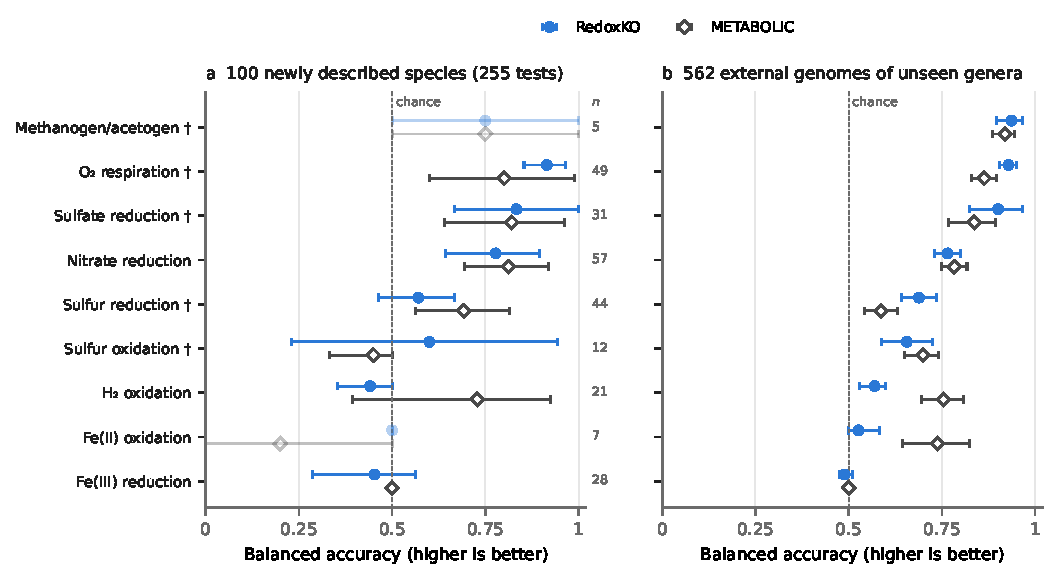
\includegraphics[width=1\linewidth,height=\textheight,keepaspectratio,alt={RedoxKO and METABOLIC by category. Balanced accuracy, the mean of sensitivity and specificity, on (a) 100 new species and (b) 562 external genomes. Bars are 95\% bootstrap intervals over description papers (a) or genomes (b). † marks categories in which RedoxKO gives yes/no calls, and lighter rows have fewer than ten tests (n, the number of tests in a). Categories with fewer than two tests or without labels are not shown. The dashed line marks random guessing. Values for (b) are in Supplementary Table .}]{figures/Fig_new_species_per_category.pdf}
\caption{\textbf{RedoxKO and METABOLIC by category.} Balanced accuracy,
the mean of sensitivity and specificity, on (a) 100 new species and (b)
562 external genomes. Bars are 95\% bootstrap intervals over description
papers (a) or genomes (b). † marks categories in which RedoxKO gives
yes/no calls, and lighter rows have fewer than ten tests (\emph{n}, the
number of tests in a). Categories with fewer than two tests or without
labels are not shown. The dashed line marks random guessing. Values for
(b) are in Supplementary Table \ref{tab:s_metabolic}.}\label{fig:percat}
\end{figure}

\subsection{Confidence labels mark the more reliable
calls}\label{confidence-labels-mark-the-more-reliable-calls}

We tested whether the confidence labels keep their coverage on genomes
the models have not seen, in the categories that get yes/no calls
(Supplementary Table \ref{tab:s_conformal}). On new species, the labels
reached the 90\% target, with lower coverage for negative than for
positive tests. On the external genomes, whose labels come from the
larger dataset, coverage was slightly below the target, mainly because
of negative labels. Half to two thirds of the predictions (49\% to 67\%)
received a confident label. On new species these were more often correct
than the yes/no calls, but on the external genomes they were not.

For the unlabeled genomes of the focused collection, the workflow
returns calibrated scores, yes/no calls where the release rule allows
them, and confidence labels. Because predictions are less reliable for
distant organisms, each output also states whether the genome's genus
and family occur among the training genomes, as PICRUSt2 does with its
distance to reference genomes \autocite{Douglas2020}. These predictions
help decide what to test in the laboratory, but only growth experiments
can confirm them.

\subsection{MAGs give nearly the same predictions as
isolates}\label{mags-give-nearly-the-same-predictions-as-isolates}

Many organisms are known only from MAGs, which often miss part of the
genome. Genome-based trait predictors have been applied to such genomes
\autocite{Weimann2016,Weissman2021}, and we checked how much the missing
genes change the predictions. We compared the predictions for each MAG
with those for an isolate genome of the same species (Supplementary
Table \ref{tab:s_mags}). The MAG and the isolate received nearly the
same calls at every completeness level, and agreement was only slightly
lower below 90\% completeness. There, about one in ten positive calls of
the isolate was lost in the MAG. EnergyKO-M agreed most often, also for
isolates outside its training set. MAGs of at least medium quality by
the MIMAG standard, that is, at least 50\% complete
\autocite{Bowers2017}, can therefore be used much like isolates, but a
missing call in an incomplete MAG is weaker evidence than in an isolate.

To illustrate use on uncultured organisms, we predicted the donor and
acceptor potential of 300 high-quality MAGs from five habitats, sampling
at most one MAG per genus to limit taxonomic redundancy. A previous
study addressed this question with marker genes in one environment
\autocite{Anantharaman2016}, and this analysis extends it to five. All
five expectations recorded before the analysis were confirmed for
RedoxKO, each significant after BH correction (Fig. \ref{fig:mags}). As
expected, hydrogen-oxidation scores were higher in hydrothermal-vent
MAGs than in seawater MAGs, and sulfur oxidation was predicted more
often there than in human-gut MAGs. Iron-oxidation scores were higher in
acid mine drainage than in each other habitat. Methanogens and acetogens
were predicted more often in anaerobic digesters than in seawater, and
oxygen respiration more often in seawater than in the gut or in
digesters. Hydrogen oxidation has no calls after the change to the
release rule, so its expectation was tested on scores, like Fe(II)
oxidation. With RedoxKO-LX, with which the expectations were registered,
four of the five held, and the difference for methanogens and acetogens
was not significant. Because these expectations follow from textbook
physiology, the analysis shows that the predictions make biological
sense. It does not test whether each prediction is correct.

Some predictions made less biological sense. RedoxKO gave high
hydrogen-oxidation scores to most gut and digester MAGs, consistent with
fermentative {[}FeFe{]} and group 3 hydrogenases sharing KOs with uptake
hydrogenases \autocite{Greening2016}. A high hydrogen-oxidation score
therefore shows only that a genome has hydrogenase genes.

\begin{figure}
\centering
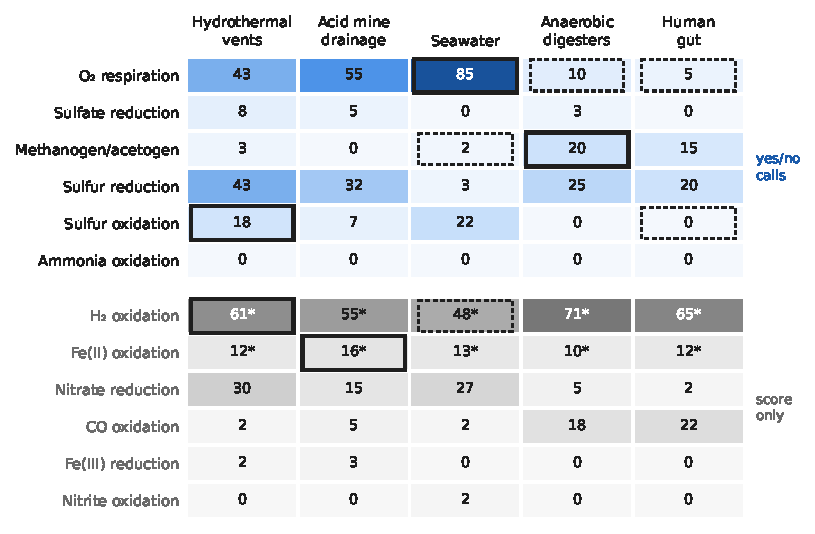
\includegraphics[width=0.85\linewidth,height=\textheight,keepaspectratio,alt={Predicted capabilities of 300 MAGs from five habitats. Percentage of the 60 MAGs per habitat called positive by RedoxKO (*median score ×100 where tested on scores). Blue rows have yes/no calls, grey rows scores only, cut at the cross-validation threshold. Solid outlines mark the habitat expected to be higher, dashed outlines the comparison habitat. Other donors and other acceptors are not shown.}]{figures/Fig_mags_habitats.pdf}
\caption{\textbf{Predicted capabilities of 300 MAGs from five habitats.}
Percentage of the 60 MAGs per habitat called positive by RedoxKO
(*median score ×100 where tested on scores). Blue rows have yes/no
calls, grey rows scores only, cut at the cross-validation threshold.
Solid outlines mark the habitat expected to be higher, dashed outlines
the comparison habitat. Other donors and other acceptors are not
shown.}\label{fig:mags}
\end{figure}

\subsection{Pathway traits are predicted moderately, and a module rule
does almost as well on new
species}\label{pathway-traits-are-predicted-moderately-and-a-module-rule-does-almost-as-well-on-new-species}

We next tested whether the approach also predicts more specific traits,
the energy-metabolism pathways. Across the 20 pathway traits, EnergyKO-M
ranked genomes better than both the taxonomic baseline and a rule based
on module completeness alone (Table \ref{tab:pathway}). Neither another
learner nor a narrower training set clearly improved it. Extra-trees,
added after the protocol was registered, scored about as well in
cross-validation but ranked new species less well (Table
\ref{tab:pathway}). Training only on autotroph-like genomes lowered
accuracy slightly in cross-validation and did not change the ranking of
new species significantly, also for autotroph-like species
(Supplementary Table \ref{tab:s_pathway_auto}). Performance varied
widely between traits (Supplementary Table \ref{tab:s_pathway_traits}).
Methanogenesis and nitrate reduction were predicted best, whereas traits
that lack a defined KEGG module or whose labels were largely predicted
from taxonomy, such as arsenate and manganese reduction, were predicted
poorly. On newly described species, EnergyKO-M and EnergyKO-BF ranked
about two in three positive growth experiments above negative ones but
gave weak yes/no calls (Table \ref{tab:pathway}). Here the module rule
ranked almost as well as the learned models, whereas the taxonomic
baseline did no better than chance. No genus of these species occurs
among the training genomes, and for pathway traits the higher taxonomic
ranks carried little information.

Module completeness helps to explain the scores. Genomes labeled
positive for a process usually carried a much more complete version of
the matching KEGG module than negatives, most clearly for dissimilatory
sulfate reduction and nitrification (Supplementary Table
\ref{tab:s_modules}). The modules also separate denitrification from
dissimilatory nitrate reduction to ammonium, which the donor and
acceptor scheme merges into one category.

\par

\penalty-100\begingroup\dimen0=24\baselineskip\dimen2=\pagegoal\advance\dimen2-\pagetotal\ifdim\dimen0>\dimen2\ifdim\dimen2>0pt\vfil\fi\penalty-10000\fi\endgroup

\begingroup\small\hyphenpenalty=10000\renewcommand{\arraystretch}{1.25}

\begin{longtable}[]{@{}
  >{\raggedright\arraybackslash}p{(\linewidth - 10\tabcolsep) * \real{0.3059}}
  >{\raggedright\arraybackslash}p{(\linewidth - 10\tabcolsep) * \real{0.2824}}
  >{\raggedleft\arraybackslash}p{(\linewidth - 10\tabcolsep) * \real{0.0941}}
  >{\raggedleft\arraybackslash}p{(\linewidth - 10\tabcolsep) * \real{0.1059}}
  >{\raggedleft\arraybackslash}p{(\linewidth - 10\tabcolsep) * \real{0.1059}}
  >{\raggedleft\arraybackslash}p{(\linewidth - 10\tabcolsep) * \real{0.1059}}@{}}
\caption{\textbf{Pathway models.} Macro AUPRC over 20 traits on 3,378
genomes in cross-validation, and macro AUROC and MCC on 99 newly
described species (203 growth experiments). Bold marks the best value in
each column. \textsuperscript{a}In cross-validation trained on three of
five folds, because one fold was used to stop training early, so not
directly comparable. \label{tab:pathway}}\tabularnewline
\toprule\noalign{}
\begin{minipage}[b]{\linewidth}\raggedright
Model
\end{minipage} & \begin{minipage}[b]{\linewidth}\raggedright
Features
\end{minipage} & \begin{minipage}[b]{\linewidth}\raggedleft
Genus-level CV
\end{minipage} & \begin{minipage}[b]{\linewidth}\raggedleft
Family-level CV
\end{minipage} & \begin{minipage}[b]{\linewidth}\raggedleft
New species AUROC
\end{minipage} & \begin{minipage}[b]{\linewidth}\raggedleft
New species MCC
\end{minipage} \\
\midrule\noalign{}
\endfirsthead
\toprule\noalign{}
\begin{minipage}[b]{\linewidth}\raggedright
Model
\end{minipage} & \begin{minipage}[b]{\linewidth}\raggedright
Features
\end{minipage} & \begin{minipage}[b]{\linewidth}\raggedleft
Genus-level CV
\end{minipage} & \begin{minipage}[b]{\linewidth}\raggedleft
Family-level CV
\end{minipage} & \begin{minipage}[b]{\linewidth}\raggedleft
New species AUROC
\end{minipage} & \begin{minipage}[b]{\linewidth}\raggedleft
New species MCC
\end{minipage} \\
\midrule\noalign{}
\endhead
\bottomrule\noalign{}
\endlastfoot
\emph{Learned models} & & & & & \\*
\quad Extra-trees & KO profile & \textbf{0.506} & 0.433 & 0.602 &
0.148 \\
\quad EnergyKO-M & KO profile + modules & 0.501 & 0.454 & 0.673 &
0.193 \\
\quad EnergyKO & KO profile & 0.500 & \textbf{0.459} & 0.650 &
\textbf{0.218} \\
\quad EnergyKO-BF & KO profile + Bacformer & 0.486 & 0.426 &
\textbf{0.701} & 0.179 \\
\quad KO panel model & 852 KOs & 0.467 & 0.424 & 0.628 & 0.175 \\
\quad Bacformer, fine-tuned\textsuperscript{a} & Bacformer-large & 0.356
& 0.289 & 0.618 & 0.178 \\
\emph{Baselines} & & & & & \\*
\quad Taxonomic baseline & taxonomy & 0.340 & 0.281 & 0.502 & 0.061 \\
\quad KEGG module rule & module completeness & 0.213 & 0.213 & 0.660 &
0.154 \\
\end{longtable}

\endgroup

\subsection{LLMs predict well mainly when given the organism
name}\label{llms-predict-well-mainly-when-given-the-organism-name}

Finally, we tested whether LLMs can read the same gene evidence
(Supplementary Table \ref{tab:s_llm}). Given anonymized gene evidence,
both LLMs predicted donors and acceptors better than the taxonomic
baseline but worse than the trained models. When the organism name was
added, they reached or exceeded the trained models, and for pathways the
name mattered even more. Given the organism name and no web search, an
LLM therefore answers mainly from what it already knows about this
organism. This is useful for summarizing existing knowledge, for example
through TogoMCP, but it does not show how well an LLM would predict the
metabolism of an organism that has not yet been studied. Our experiments
do not show how the LLMs used the name.

\section{Discussion}\label{discussion}

The main outcome of the hackathon was a shared workflow connecting
sequence-derived annotations with physiological evidence. The RDF
resource supplies identifiable proteins, KO assignments, and functional
descriptions. Literature-assisted curation supplies candidate phenotype
labels and supporting statements. Visualization makes agreement and
conflict inspectable, and the benchmark tests prediction beyond labeled
training groups. Module annotations provide additional biological
context for interpreting broad trait categories.

TogoMCP and supervised prediction have complementary roles in this
workflow. TogoMCP supports flexible evidence gathering about
characterized organisms, while the trained models provide reproducible
scores when physiological information is unavailable. The predictor
already reports, for each category, a calibrated score, a call where the
category is reliable, a confidence label and whether the genus and
family of the queried genome were represented in training. Exposing it
as an MCP tool alongside the annotations is the next step.

\subsection{Implications for model development and data
curation}\label{implications-for-model-development-and-data-curation}

On newly described species, the models reached only moderate accuracy.
They ranked about three in four positive growth experiments above
negative ones and detected about half of the donors and acceptors found
in growth experiments (Table \ref{tab:newspecies}). This accuracy was,
however, measured in a strict test. The test genera were absent from
training, and the labels came from a different source, the published
growth experiments. Accuracy falls as test genomes become more distant
from training \autocite{Hackmann2026}, and RedoxKO itself scored higher
with a random split than in genus-level cross-validation. Our estimates
are therefore closer to what a user can expect for an organism that has
not yet been studied.

In our tests, the model architecture mattered little. Neither the
deep-learning variants we tested nor automated model search clearly
exceeded RedoxKO, a random forest on the KO panel (Supplementary Table
\ref{tab:s_dl}). This included models pretrained on large unlabeled
datasets, such as fine-tuned Bacformer-large, self-supervised
pretraining on unlabeled genomes and the tabular foundation model TabPFN
\autocite{Hollmann2025}. Instead, accuracy grew with the number of
labeled genera (Fig. \ref{fig:learning}). The curve rests on four sizes
and was flat between the second and third, but more labeled genomes may
help more than new architectures. Label errors and missing marker genes
could also limit accuracy. Genome language models trained at larger
scale \autocite{Hwang2024,Nguyen2024} may also become more accurate as
more labeled genomes become available.

However, additional data helped only when they matched the training data
(Supplementary Table \ref{tab:s_registered}). The full KO profile did
not rank new species better than the KO panel. Adding genomes labeled
from the larger dataset made the ranking of nitrate tests on new species
worse, probably because that dataset defines nitrate reduction more
broadly and labels most of these genomes positive.

The labels also limit the models in a second way. A trait not reported
in the literature counts as absent. We attribute to this the cautious
thresholds of the models, which detected only about half of the donors
and acceptors that new species used in growth experiments (Table
\ref{tab:newspecies}). Hiding positives in the training labels barely
changed the ranking, whereas hiding them in the test labels lowered the
measured score (Supplementary Fig. \ref{fig:s_noise}), so our measured
scores may underestimate how well the models rank. We tried three ways
to correct this (Supplementary Table \ref{tab:s_registered}). First,
shifting decision thresholds by the estimated reporting rate found more
true positives on new species, but did not improve the calls
significantly and made them worse on the external genomes. Second,
positive-unlabeled bagging \autocite{Mordelet2014}, which treats
unreported traits as unknown, did not improve ranking on new species.
Third, we re-read the literature for the training species with an LLM,
with every claim tied to a quoted string. This resolved only a small
share of the unreported traits, because species descriptions state what
an organism uses but rarely what was tested and not used. None of these
corrections helped. The missing negatives cannot be recovered from the
existing literature, so our cross-validation scores measure how well the
models predict reported traits. A possible solution is to obtain
negative labels from standard growth tests, which automated cultivation
platforms could run for many organisms at once \autocite{Huang2023}.

On newly described species, METABOLIC's yes/no calls were at least as
accurate as those of RedoxKO. Pooled over all tests METABOLIC was ahead,
and averaged over categories the two were equal. Neither difference was
significant, but the interval also allows a clear lead for METABOLIC.
Accuracy can also make a tool that calls many tests positive look better
than it is, because most published tests are positive. For example,
METABOLIC called every Fe(III)-reduction test positive, which looks
accurate for this reason but does not separate positives from negatives.
On the external genomes, RedoxKO could rank genomes and its calls had a
higher MCC, because it made fewer false-positive calls, whereas the
balanced accuracy of the two tools' calls was similar.

The two kinds of tool answer different questions. A rule tells whether
the genes of a pathway are present, whereas a learned score ranks
genomes by how likely they are to use the pathway. Because RedoxKO's
scores separated true from false positives even among METABOLIC's own
positive calls, the two can be used together. Rules then provide the
yes/no annotation, especially when missed positives are costly and for
organisms far from the training genomes, where METABOLIC's calls lost
less accuracy. Learned scores help to screen large genome collections,
to decide which genomes to test first and to avoid costly false
positives. RedoxKO also runs about three times faster than METABOLIC
(Supplementary Table \ref{tab:s_registered}). Neither kind of tool,
however, predicts iron and manganese metabolism well enough. For these
categories, new genomic markers of extracellular electron transfer will
be needed first.

\begin{figure}
\centering
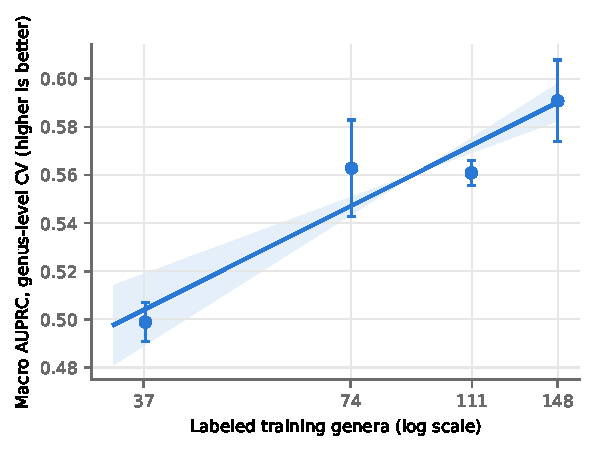
\includegraphics[width=0.6\linewidth,height=\textheight,keepaspectratio,alt={Relationship between accuracy and the amount of labeled data. RedoxKO in genus-level cross-validation. Points are means of three random subsamples of genera (at full size, the six fold allocations of Supplementary Table ), with standard deviations as error bars. The blue line is a log-linear fit, with the 95\% interval of its slope shaded.}]{figures/Fig_learning_curve.pdf}
\caption{\textbf{Relationship between accuracy and the amount of labeled
data.} RedoxKO in genus-level cross-validation. Points are means of
three random subsamples of genera (at full size, the six fold
allocations of Supplementary Table \ref{tab:s_splits}), with standard
deviations as error bars. The blue line is a log-linear fit, with the
95\% interval of its slope shaded.}\label{fig:learning}
\end{figure}

\subsection{Prospects for cultivation and biological
discovery}\label{prospects-for-cultivation-and-biological-discovery}

Compatible donor, acceptor, and carbon fixation predictions could help
prioritize substrate combinations for experimental screening. For
example, evidence of sulfur oxidation together with respiratory nitrate
reduction could motivate testing sulfur-containing electron donors with
nitrate as an acceptor. The relevant functions must nevertheless operate
together under suitable conditions, and assimilatory transformations
must be distinguished from energy-conserving respiration.

Actual medium design additionally depends on nutrient requirements,
temperature, pH, substrate concentrations, toxicity, and regulation.
Neither KO presence nor module completeness establishes active
metabolism, and missing annotations in a MAG may reflect incomplete
reconstruction rather than true gene absence. In our tests, predictions
from MAGs at least 50\% complete agreed closely with those from
isolates, slightly less so below 90\% completeness. Our focus on known
autotrophs also limits extrapolation to other lifestyles. We did not
experimentally validate cultivation predictions during this work.
Predictions were evaluated on newly described species and on
metagenome-assembled genomes, but testing defined substrate combinations
in cultured strains is still necessary to establish practical utility.

\subsection{Limitations}\label{limitations}

The main limitations lie in the labels. Training labels count a category
not reported in the literature as negative, although most such negatives
were never tested, and the literature can resolve only few of them. We
attribute the cautious thresholds and low sensitivity of the models to
these labels. The labeled set is also small, especially for the rarest
categories (Supplementary Table \ref{tab:s_datasets}), so results for
these categories are uncertain. For most pathway traits, nearly all
positives come from records that cite FAPROTAX, which assigns traits by
taxon (Supplementary Table \ref{tab:s_pathway_traits}). Part of what the
pathway models learn is therefore the taxonomy of the organism. Several
external labels also come from FAPROTAX, and the larger dataset serves
both as the external test for donors and acceptors and as the source of
pathway labels, so these evaluations are not fully independent.

The test on new species has its own limits. The species come from papers
that report which electron donors and acceptors they use, and most of
their evidence comes from abstracts, so the tests may over-represent
positive results. We designed the extraction so that it could not see
model output, but this cannot be proven. The withheld species provide
too few tests to detect anything but large differences between models
(Supplementary Table \ref{tab:s_registered}), and the pretrained
sequence models may have seen some test genomes during pretraining.
RedoxKO became the final model after the tests on the external genomes
and new species, so its results on these sets are not blind. Two later
blind tests of the frozen model gave similar ranking, but they contained
few negative tests for electron donors and showed no advantage of
RedoxKO over RedoxKO-LX (Supplementary Table \ref{tab:s_blind}). In
cross-validation, a nearest-neighbor rule on KO content came close to
RedoxKO, so part of what the models learn is overall similarity in gene
content. Only on the external genomes did RedoxKO clearly exceed this
rule. The results of RedoxKO-LX, chosen before these tests, are given
beside them (Tables \ref{tab:cv} and \ref{tab:newspecies}). Finally, the
predictions show which processes a genome encodes. Whether the organism
carries them out in a given environment needs growth experiments to
show.

A single kind of new data could solve most of these limitations. Growth
experiments that record negative as well as positive outcomes, on
organisms chosen from many genera, would provide both better training
labels and a prospective test free of literature reporting bias.

\section{Conclusions}\label{conclusions}

During BioHackathon 2026, we developed resources linking microbial
genome annotations to electron donor and acceptor information, made
genomic evidence accessible through TogoMCP, and evaluated several
approaches to trait prediction. Gene content alone gave most of the
accuracy we observed and held up on genera and species absent from
training and on metagenome-assembled genomes. Adding a genome language
model gave a small gain in cross-validation that was not significant
against the KO ensemble it extends and did not carry over to the
external genomes. The rule-based tools METABOLIC and DRAM gave yes/no
calls at least as accurate. Pathway annotations and phenotype
disagreements offered complementary routes for inspecting predictions,
and the categories where prediction fails, chiefly extracellular metal
reduction, show where new genomic markers and better labels are most
needed. The resulting resources provide a basis for reproducible
screening, continued curation, and experimental testing of
genome-informed cultivation hypotheses.

\section{Data and software
availability}\label{data-and-software-availability}

The manuscript repository is BH26-microbial-metabolic-traits. The
microbial annotation resource was integrated with TogoMCP, whose source
repository documents the service. The electron\_predictor repository
provides marker-matching software and an autotroph viewer.

The analysis outputs include model artifacts, metric tables, split
assignments, and predictions for genomes without benchmark labels. Code,
trained models, frozen cross-validation splits, evaluation sets and all
metric tables are available at \textcolor{red}{[GitHub URL]} and
archived at Zenodo (\textcolor{red}{[DOI]}). The released models, with
SHA-256 hashes, are the donor and acceptor models RedoxKO (file RF, 36
MB), RedoxKO-LX (B2, 8.5 MB) and RedoxKO-ens-BF (B2XLE\_large, 13 MB)
and the pathway models EnergyKO-M (PB3, 19 MB) and EnergyKO-BF (PE).
Supplementary Table \ref{tab:s_models} lists them and when to use each.
A prediction script accepts RefSeq accessions or nucleotide FASTA and
adds confidence labels to its output. The release also contains the
genome accession lists and the test sets of newly described species,
with every growth experiment, its source and quoted string. It further
contains the MAG-isolate pairs and habitat MAG lists from GTDB release
232, the calls of every comparator tool, and all pre-registration
documents with their hashes.

\section{Acknowledgements and
declarations}\label{acknowledgements-and-declarations}

We thank the BioHackathon 2026 organizers and participants and the
maintainers of the resources used here. {[}TO CONFIRM: author
contributions, funding, and competing interests.{]} LLMs assisted
evidence extraction, trait prediction experiments, and manuscript
drafting; authors must review the final text and underlying evidence.
FEDOT.MAS pipelines extracted, checked and audited the phenotype tables,
with DeepSeek V4 Pro or Claude Opus 5 coordinating Gemini 3.7 Flash,
Gemini 3.8 Flash or GPT-5.6 Luna. In the prediction part, LLMs were used
in three ways. First, Claude Opus 5 and GPT-6 Astra were compared with
the trained models, as described in the Methods (prompts, inputs and raw
outputs are released). Second, LLM agents extracted the growth
experiments of the newly described species, each with a quoted string
from its source. Third, Claude Haiku 5.5 re-read the literature for the
training species, with every claim checked against a quoted string. All
reported numbers are produced by code in the released repository.

\AtEndDocument{%

\section{Appendices}\label{appendices}

\setcounter{table}{0}\renewcommand{\thetable}{S\arabic{table}}\renewcommand{\theHtable}{S\arabic{table}}
\setcounter{figure}{0}\renewcommand{\thefigure}{S\arabic{figure}}\renewcommand{\theHfigure}{S\arabic{figure}}
\captionsetup{singlelinecheck=false}

The following material supports the prediction sections. Code, result
files and all pre-registration documents are in the repository.

\subsection{Supplementary Note 1. Deviations from the registered
protocol}\label{supplementary-note-1.-deviations-from-the-registered-protocol}

We registered the donor and acceptor protocol on 17 September 2026,
before scoring the first model, and followed it with the changes
described below.

\emph{Additional sensitivity analyses.} On 17 September, after the first
internal audit and before any sequence model was scored, we added four
sensitivity analyses. The audit had found likely label errors among the
negatives, so one analysis treats a genome's donor or acceptor labels as
missing when all of them are negative. Because the registered folds used
NCBI taxonomy, a second analysis rebuilds the folds from GTDB taxonomy.
The other two add five further fold allocations and keep only genomes of
high assembly quality. At the same time, we decided to report two models
as tied when the interval of their paired difference includes zero. We
also decided to base the main claims on macro averages and to correct
for multiple testing with the Benjamini-Hochberg method within each
group of tests. A second macro average, over 12 categories, leaves out
other donors and other acceptors. The 14-category average remains the
main measure. These additions did not change any registered analysis.
They were run with RedoxKO-LX, the final model at the time, which stayed
ahead of the taxonomic baseline in all of them. Supplementary Table
\ref{tab:s_splits} gives the results.

\emph{Choice of the final model.} After the second internal audit, on 18
September, we added a rule for replacing the final model, then
RedoxKO-LX. A new model replaces it only if it scores higher in
cross-validation and does not score lower on the external genomes in any
reported subset. We wrote this rule together with the external test.
RedoxKO-ens scored higher in cross-validation but failed the rule,
because it scored significantly lower on the external genomes whose
labels do not come from FAPROTAX (Supplementary Table
\ref{tab:s_paired}). On all external genomes the two were tied. We then
applied the same check to all registered models. Bacformer-large alone
scored about as well as RedoxKO-LX in genus-level cross-validation,
lower at family level and significantly lower on the external genomes.
We added this step after the cross-validation ranking was known,
although the external comparison had already been planned and computed.
It changed which model became the final model, but not any reported
value.

\emph{Switch to the random forest.} We had trained a random forest on
the same 852 KOs as a comparison model but had not applied this rule to
it. On 21 October, after all other analyses had been done, we applied
the rule to it. In genus-level cross-validation the random forest scored
higher than RedoxKO-LX, but the interval of the difference included
zero, so by our definition the two were tied (Supplementary Table
\ref{tab:s_paired}). The switch therefore rested on two results. The
random forest scored significantly higher on the external genomes, also
on those whose labels do not come from FAPROTAX, and its yes/no calls on
the 100 primary new species were significantly more accurate. The 43
withheld species were not used. It became the final model, RedoxKO, and
the former final model was renamed RedoxKO-LX. We then repeated every
analysis of the final model with the random forest. Because the switch
was made after all test results were known, the results of RedoxKO on
the external genomes and new species are not blind. The experiments
registered in advance had been run with RedoxKO-LX. We repeated them
with RedoxKO and report the repeats in Supplementary Table
\ref{tab:s_registered}. The original results remain in the repository.

\emph{Fourth condition of the release rule.} On 22 October we added a
fourth condition to the release rule: where the external genomes have
labels for a category, the MCC of its calls on them must exceed 0.2.
Only hydrogen oxidation failed it (Supplementary Table
\ref{tab:s_release}), so it now returns a score only, and its habitat
expectation was tested on scores, as the registration prescribes for
categories without calls. We made this change after all results were
known.

\emph{Blind tests of the frozen model.} On 22 October we froze RedoxKO
with its release rule, recorded the hashes of the model files and
registered two blind tests before searching for species (Supplementary
Table \ref{tab:s_blind}). The first used species described in 2026. Its
registered search window, 15 September to 22 October, gave no eligible
species, so before extraction we widened it to the whole year. The
second used description papers of lithotrophs from any year. Only eight
species came from genera absent from all project data, so before
extraction we added species from genera absent from the training
genomes. In both tests we corrected the quote check and the rule for
statements that are not growth experiments before scoring. After scoring
we restricted the yes/no calls to the six categories that get them, as
registered. Both tests are reported regardless of their outcome.

\emph{Pathway task.} On 18 September we added the pathway task with its
own registration, labels, genomes and frozen folds. Nothing in the donor
and acceptor analysis was rerun or chosen again because of it.

\emph{Alternative models.} On 21 and 22 September, after the test on
newly described species, in which RedoxKO-ens-BF and EnergyKO-BF did not
differ significantly from the final models, we also named these two as
alternative models. The final models did not change.

\emph{LLM comparison.} We did not keep the transcripts of the isolated
Claude agents that ran on 17 and 20 September, so only their final
answers are available.

\emph{Further experiments.} From 14 to 21 October we registered further
experiments before running them. Their results are reported in
Supplementary Table \ref{tab:s_registered} regardless of their outcome.

\subsection{Supplementary Note 2. Audit of the phenotype
collection}\label{supplementary-note-2.-audit-of-the-phenotype-collection}

In October 2026 we checked the phenotype collection against its cited
sources and classified the errors as in a study of LLM-assisted data
extraction \autocite{Gartlehner2025}. Supplementary Table
\ref{tab:s_audit} lists them. In the separate donor and acceptor table,
nearly all errors concerned the format of quotes. After the corrections,
we re-checked a stratified random sample of 300 items against the
sources. Of the 239 sampled values graded A to C that could be checked
against an open source, 2.1\% still had a major error and 18.0\% had an
error of any kind. Gartlehner et al.~found major errors in 2.5\% of
LLM-assisted and 2.7\% of human-only extractions. Every error found in
the sample was corrected. The audit changed 17 of the 3,828 training
labels that it could match by name. Re-scoring the cross-validation
predictions with the corrected labels changed macro AUPRC by at most
0.004.

\subsection{Supplementary Note 3. Agreement between the two label
sources}\label{supplementary-note-3.-agreement-between-the-two-label-sources}

Comparing the two label sources shows how much the evaluations depend on
the labels. For the species in both, the labels of the phenotype
collection and the larger dataset agreed moderately, and RedoxKO agreed
with the larger dataset slightly less (Supplementary Table
\ref{tab:s_concordance}). Most of the disagreement came from hydrogen
oxidation, which the phenotype collection assigned to far more species
than the larger dataset. Without it, the two sources agreed well. The
sources therefore differ in what they label and in how much evidence
they cover. They are also not fully independent, because most of the
shared species have records from FAPROTAX in the larger dataset, which
assigns traits from the organism's taxonomy.

The comparison also found genomes labeled negative for a trait although
their marker genes or other records indicated its presence. For example,
five genomes with a complete methyl-coenzyme M reductase (\emph{mcrABG})
were labeled as non-methanogens, and nine strictly aerobic ammonia or
nitrite oxidizers were labeled as not respiring oxygen. Such cases are
candidates for re-curation with the viewer and other sources. A
prediction supported by marker genes does not prove a labeling error,
because gene regulation, pathway direction, growth conditions and strain
differences can also explain a disagreement.

\subsection{Supplementary tables}\label{supplementary-tables}

Square brackets give 95\% bootstrap confidence intervals, resampled over
genera or families in cross-validation, over genera for the external
genomes and over the description papers for new species.

\begingroup\hyphenpenalty=10000\small\renewcommand{\arraystretch}{1.35}\setlength{\tabcolsep}{5pt}

\begin{longtable}[]{@{}
  >{\raggedright\arraybackslash}p{(\linewidth - 8\tabcolsep) * \real{0.2449}}
  >{\raggedright\arraybackslash}p{(\linewidth - 8\tabcolsep) * \real{0.2347}}
  >{\raggedright\arraybackslash}p{(\linewidth - 8\tabcolsep) * \real{0.0918}}
  >{\raggedright\arraybackslash}p{(\linewidth - 8\tabcolsep) * \real{0.2245}}
  >{\raggedright\arraybackslash}p{(\linewidth - 8\tabcolsep) * \real{0.2041}}@{}}
\caption{\textbf{Datasets used in this study.} All genomes are isolates
except the MAGs. \label{tab:s_datasets}}\tabularnewline
\toprule\noalign{}
\begin{minipage}[b]{\linewidth}\raggedright
Dataset
\end{minipage} & \begin{minipage}[b]{\linewidth}\raggedright
Source and selection
\end{minipage} & \begin{minipage}[b]{\linewidth}\raggedright
Genomes
\end{minipage} & \begin{minipage}[b]{\linewidth}\raggedright
Labels
\end{minipage} & \begin{minipage}[b]{\linewidth}\raggedright
Use
\end{minipage} \\
\midrule\noalign{}
\endfirsthead
\toprule\noalign{}
\begin{minipage}[b]{\linewidth}\raggedright
Dataset
\end{minipage} & \begin{minipage}[b]{\linewidth}\raggedright
Source and selection
\end{minipage} & \begin{minipage}[b]{\linewidth}\raggedright
Genomes
\end{minipage} & \begin{minipage}[b]{\linewidth}\raggedright
Labels
\end{minipage} & \begin{minipage}[b]{\linewidth}\raggedright
Use
\end{minipage} \\
\midrule\noalign{}
\endhead
\bottomrule\noalign{}
\endlastfoot
\emph{Training} & & & & \\*
\quad Donor/acceptor & Phenotype collection (this study), extracted from
published papers, focused set of autotrophs & 358 & 14 categories,
12-208 positives per category (3-58\%) & Cross-validation \\
\quad Pathways & Larger dataset \autocite{Madin2020}, species with
pathway labels, one genome per species & 3,378 & 20 traits, 30-1,814
positives per trait (1-54\%) & Cross-validation \\
\emph{Evaluation} & & & & \\*
\quad External genomes & Larger dataset, genera absent from
donor/acceptor training & 562 & 9 categories, 19-289 positives per
category (3-62\% of the genomes labeled for it) & Test on unseen
genera \\
\quad New species & Described 2015-2026, genus absent from all project
data, one per genus in the primary set of 100, and 43 withheld species &
143 & 330 experiments, 61\% positive & Test on new species \\
\quad New species, pathways & Same selection & 99 & 203 experiments,
53\% positive & Test on new species \\
\quad New species, autotroph-like & 70 autotroph-like species of the 143
plus 29 taken from description papers of 2000-2026, extracted the same
way & 99 & 220 experiments & Registered autotroph test \\
\quad MAG-isolate pairs & GTDB release 232 \autocite{Parks2022}, MAGs ≥
50\% complete and ≤ 10\% contaminated, one per species and completeness
bin, paired with 222 isolates & 372 MAGs & Isolate predictions & Effect
of completeness \\
\emph{Applications and resources} & & & & \\*
\quad Habitat MAGs & GTDB release 232, ≥ 90\% complete and ≤ 5\%
contaminated, one per genus, five habitats & 300 & None, uncultured &
Habitat comparison \\
\quad Unlabeled genomes & Focused collection without labels & 228 &
None, no published evidence & Predictions \\
\quad LLM subset & Stratified sample of training genomes & 96 & 14
categories, 20 traits & Comparison with LLMs \\
\quad Shared KO resource & KofamScan annotations of RefSeq genomes,
available through TogoMCP & 23,434 & KO annotations only & Annotation
source \\
\end{longtable}

\endgroup

\begingroup\hyphenpenalty=10000\small\renewcommand{\arraystretch}{1.35}\setlength{\tabcolsep}{5pt}

\begin{longtable}[]{@{}
  >{\raggedright\arraybackslash}p{(\linewidth - 8\tabcolsep) * \real{0.3827}}
  >{\raggedleft\arraybackslash}p{(\linewidth - 8\tabcolsep) * \real{0.2222}}
  >{\raggedleft\arraybackslash}p{(\linewidth - 8\tabcolsep) * \real{0.1481}}
  >{\raggedleft\arraybackslash}p{(\linewidth - 8\tabcolsep) * \real{0.0988}}
  >{\raggedleft\arraybackslash}p{(\linewidth - 8\tabcolsep) * \real{0.1481}}@{}}
\caption{\textbf{Performance of RedoxKO on genomes with and without a
carbon-fixation pathway.} Autotroph-like genomes have a KEGG module for
carbon fixation or methanogenesis at least 80\% complete.
\textsuperscript{a}Collected for this test, 220 growth experiments, MCC
0.41. \label{tab:s_autotroph}}\tabularnewline
\toprule\noalign{}
\begin{minipage}[b]{\linewidth}\raggedright
Test set
\end{minipage} & \begin{minipage}[b]{\linewidth}\raggedleft
Autotroph-like genomes
\end{minipage} & \begin{minipage}[b]{\linewidth}\raggedleft
Macro AUROC, autotroph-like
\end{minipage} & \begin{minipage}[b]{\linewidth}\raggedleft
Macro AUROC, other
\end{minipage} & \begin{minipage}[b]{\linewidth}\raggedleft
Difference
\end{minipage} \\
\midrule\noalign{}
\endfirsthead
\toprule\noalign{}
\begin{minipage}[b]{\linewidth}\raggedright
Test set
\end{minipage} & \begin{minipage}[b]{\linewidth}\raggedleft
Autotroph-like genomes
\end{minipage} & \begin{minipage}[b]{\linewidth}\raggedleft
Macro AUROC, autotroph-like
\end{minipage} & \begin{minipage}[b]{\linewidth}\raggedleft
Macro AUROC, other
\end{minipage} & \begin{minipage}[b]{\linewidth}\raggedleft
Difference
\end{minipage} \\
\midrule\noalign{}
\endhead
\bottomrule\noalign{}
\endlastfoot
External genomes & 285 of 562 (51\%) & 0.82 & 0.86 & −0.04 \\
New species, primary set & 46 of 100 (46\%) & 0.83 & 0.78 & +0.05 \\
New species, autotroph-like set\textsuperscript{a} & 99 & 0.76 & --- &
--- \\
\end{longtable}

\endgroup

\begingroup\hyphenpenalty=10000\footnotesize\renewcommand{\arraystretch}{1.35}\setlength{\tabcolsep}{5pt}

\begin{longtable}[]{@{}
  >{\raggedright\arraybackslash}p{(\linewidth - 6\tabcolsep) * \real{0.2828}}
  >{\raggedright\arraybackslash}p{(\linewidth - 6\tabcolsep) * \real{0.2828}}
  >{\raggedleft\arraybackslash}p{(\linewidth - 6\tabcolsep) * \real{0.1515}}
  >{\raggedright\arraybackslash}p{(\linewidth - 6\tabcolsep) * \real{0.2828}}@{}}
\caption{\textbf{Errors found in the audit of the phenotype collection.}
In round brackets, the share of the 6,880 values in the collection of
October 2026, counting each compound separately. The 1,817 records of
the September snapshot cover only donors and acceptors. Severity classes
follow the scheme of \autocite{Gartlehner2025}. Grade D, value kept
without citable support. \label{tab:s_audit}}\tabularnewline
\toprule\noalign{}
\begin{minipage}[b]{\linewidth}\raggedright
Error type
\end{minipage} & \begin{minipage}[b]{\linewidth}\raggedright
Example
\end{minipage} & \begin{minipage}[b]{\linewidth}\raggedleft
Collection
\end{minipage} & \begin{minipage}[b]{\linewidth}\raggedright
Outcome in the collection
\end{minipage} \\
\midrule\noalign{}
\endfirsthead
\toprule\noalign{}
\begin{minipage}[b]{\linewidth}\raggedright
Error type
\end{minipage} & \begin{minipage}[b]{\linewidth}\raggedright
Example
\end{minipage} & \begin{minipage}[b]{\linewidth}\raggedleft
Collection
\end{minipage} & \begin{minipage}[b]{\linewidth}\raggedright
Outcome in the collection
\end{minipage} \\
\midrule\noalign{}
\endhead
\bottomrule\noalign{}
\endlastfoot
\textbf{\emph{Major}} & \emph{Record says something wrong} &
\textbf{\emph{158 (2.3\%)}} & \\
\quad Wrong organism or strain & Quote about another species described
in the same paper & 86 (1.2\%) & 78 fixed, 5 removed, 3 grade D \\
\quad Wrong role & A compound the organism detoxifies taken as its
energy source & 26 (0.4\%) & 15 fixed, 3 removed, 8 grade D \\
\quad Wrong kind of value & Growth limit taken as optimum, pyrite taken
as Fe(II) & 24 (0.3\%) & 23 fixed, 1 removed \\
\quad Negation misread & ``Not used'' read as used & 11 (0.2\%) & 9
fixed, 2 removed \\
\quad Wrong value & Transcription or unit error & 11 (0.2\%) & 8 fixed,
3 grade D \\
\textbf{\emph{Minor}} & \emph{Value kept, support wrong} &
\textbf{\emph{1,955 (28.4\%)}} & \\
\quad No citable quote & Value imported from a survey sheet or curator
note without a literature quote & 1,186 (17.2\%) & 695 fixed, 12
removed, 479 grade D \\
\quad Quote does not state the value & Compound mentioned only as a
medium component & 316 (4.6\%) & 264 fixed, 15 removed, 37 grade D \\
\quad Hedged evidence graded too high & ``Genes for'', ``may'' or
``related strain'' graded as an experiment & 145 (2.1\%) & 139 fixed, 6
grade D \\
\quad Source not a publication & Link to a chat-assistant page & 124
(1.8\%) & 71 fixed, 4 removed, 49 grade D \\
\quad Quote altered & Sentence paraphrased, shortened or merged & 81
(1.2\%) & 81 fixed \\
\quad Quote not in the cited source & Correct sentence attached to the
wrong paper & 55 (0.8\%) & 54 fixed, 1 grade D \\
\quad Grade too high & Grade A resting on a single paper & 40 (0.6\%) &
38 fixed, 2 grade D \\
\quad Grade too low & A second independent source not counted & 8
(0.1\%) & 8 fixed \\
\textbf{\emph{Format only}} & \emph{Content unchanged} &
\textbf{\emph{13 (0.2\%)}} & \\
\quad Corrupted text & Characters lost in PDF text extraction & 6
(0.1\%) & 6 fixed \\
\quad Duplicate row & Same culture under a former and a current genus
name & 7 (0.1\%) & 7 removed \\
\textbf{\emph{Not assessed}} & & \textbf{\emph{430 (6.2\%)}} & \\
\quad Type not recorded & Correction by the first FEDOT.MAS validation
run & 375 (5.5\%) & 366 fixed, 9 removed \\
\quad Left to the authors & Conflicting sources or a deciding source
behind a paywall & 48 (0.7\%) & Author decision \\
\quad Other & Reason given in the error log & 7 (0.1\%) & 7 fixed \\
\textbf{Total} & & \textbf{2,556 (37.2\%)} & \textbf{1,920 fixed or
removed, 588 grade D, 48 author decision} \\
\end{longtable}

\endgroup

\begingroup\hyphenpenalty=10000\footnotesize\renewcommand{\arraystretch}{1.35}\setlength{\tabcolsep}{5pt}

\begin{longtable}[]{@{}
  >{\raggedright\arraybackslash}p{(\linewidth - 10\tabcolsep) * \real{0.2165}}
  >{\raggedright\arraybackslash}p{(\linewidth - 10\tabcolsep) * \real{0.1753}}
  >{\raggedright\arraybackslash}p{(\linewidth - 10\tabcolsep) * \real{0.1856}}
  >{\raggedright\arraybackslash}p{(\linewidth - 10\tabcolsep) * \real{0.1340}}
  >{\raggedleft\arraybackslash}p{(\linewidth - 10\tabcolsep) * \real{0.1856}}
  >{\raggedright\arraybackslash}p{(\linewidth - 10\tabcolsep) * \real{0.1031}}@{}}
\caption{\textbf{Experiments registered in advance.} Differences between
models or tools in the main measure, for RedoxKO unless another model is
named. The experiments were registered with RedoxKO-LX and repeated with
RedoxKO. Expected in advance gives the predicted outcome and, in round
brackets, our probability for it. As expected is Yes when the registered
success criterion was met. \label{tab:s_registered}}\tabularnewline
\toprule\noalign{}
\begin{minipage}[b]{\linewidth}\raggedright
Experiment
\end{minipage} & \begin{minipage}[b]{\linewidth}\raggedright
Main measure
\end{minipage} & \begin{minipage}[b]{\linewidth}\raggedright
Expected in advance
\end{minipage} & \begin{minipage}[b]{\linewidth}\raggedright
Result
\end{minipage} & \begin{minipage}[b]{\linewidth}\raggedleft
95\% CI
\end{minipage} & \begin{minipage}[b]{\linewidth}\raggedright
As expected
\end{minipage} \\
\midrule\noalign{}
\endfirsthead
\toprule\noalign{}
\begin{minipage}[b]{\linewidth}\raggedright
Experiment
\end{minipage} & \begin{minipage}[b]{\linewidth}\raggedright
Main measure
\end{minipage} & \begin{minipage}[b]{\linewidth}\raggedright
Expected in advance
\end{minipage} & \begin{minipage}[b]{\linewidth}\raggedright
Result
\end{minipage} & \begin{minipage}[b]{\linewidth}\raggedleft
95\% CI
\end{minipage} & \begin{minipage}[b]{\linewidth}\raggedright
As expected
\end{minipage} \\
\midrule\noalign{}
\endhead
\bottomrule\noalign{}
\endlastfoot
\emph{Improving RedoxKO} & & & & & \\*
\quad Adding 546 genomes from the larger dataset (84\% nitrate-positive)
& Nitrate AUROC, new species & Not stated & −0.20 & {[}−0.34,~−0.07{]} &
--- \\
\quad Thresholds shifted by the reporting rate & MCC, withheld species &
No loss & +0.08 & {[}−0.09,~+0.23{]} & Yes \\
\quad LLM re-reading of the training literature & Unreported cells
resolved & Enough to retrain & 2.4\% & & No \\
\quad Positive-unlabeled bagging & Macro AUROC, new species & Gain
unlikely (10-15\%) & −0.03 & {[}−0.11,~+0.01{]} & Yes \\
\quad No class weighting & Macro AUPRC difference, genus-level CV & None
better (about 75\% for all three) & −0.007 & {[}−0.035,~+0.026{]} &
Yes \\
\quad Undersampling of negatives to 1:1 & Macro AUPRC difference,
genus-level CV (family level +0.007) & Lower (about 65\%) & −0.025 &
{[}−0.050,~+0.015{]} & No \\
\quad Oversampling of positives to 1:1 & Macro AUPRC difference,
genus-level CV & None better & −0.015 & {[}−0.037,~+0.025{]} & Yes \\
\quad Full profile of 10,517 KOs & Macro AUROC, new species & Gain
unlikely (15-20\%) & −0.03 & {[}−0.10,~+0.03{]} & Yes \\
\quad METABOLIC's call, then RedoxKO's score & Macro AUROC vs RedoxKO,
new species & Gain likely (55-65\%) & +0.001 & {[}−0.07,~+0.07{]} &
No \\
\quad Model combining RedoxKO and METABOLIC & MCC vs METABOLIC, new
species & Gain possible (25-35\%) & −0.11 & {[}−0.24,~+0.02{]} & No \\
\quad Same model, external genomes & Macro MCC vs METABOLIC & --- &
+0.10 & {[}0.06,~0.14{]} & --- \\
\emph{RedoxKO compared with METABOLIC} & & & & & \\*
\quad Ranking within METABOLIC's positive calls & AUROC, withheld
species & Inconclusive (power 26\%) & 0.82 & {[}0.64,~1.00{]} & No \\
\quad Ranking of external genomes & Macro AUROC difference & RedoxKO
better (60-70\%) & +0.09 & {[}0.06,~0.12{]} & Yes \\
\quad Top 20 external genomes per category & Precision difference &
RedoxKO better (about 80\%) & +0.27 & {[}0.19,~0.32{]} & Yes \\
\quad Net benefit, external genomes & Difference per threshold & Depends
on the threshold & RedoxKO higher at 0.05-0.90 & & Partly \\
\quad Calls with a confident label & Accuracy difference, new species &
Even (about 50\%) & +0.01 & {[}−0.06,~+0.11{]} & Yes \\
\quad MAGs 50-70\% complete & Agreement with the isolate, RedoxKO minus
METABOLIC & RedoxKO more stable (50-60\%) & +1.9 points &
{[}−0.2,~+4.1{]} & No \\
\quad Speed & Seconds per genome & RedoxKO faster & 14.6 vs 38-60 (3.3
for the KO scan) & & Yes \\
\quad Autotroph-like new species (99) & Macro AUROC, RedoxKO & At least
0.73 (about 70\%) & 0.764 & {[}0.64,~0.86{]} & Yes \\
\quad Same species & MCC, RedoxKO & Below 0.36 (about 60\%) & 0.406 &
{[}0.27,~0.54{]} & No \\
\emph{Validity checks} & & & & & \\*
\quad External genomes without FAPROTAX labels & Macro AUROC difference
& Uncertain (about 50\%) & +0.16 & {[}0.13,~0.18{]} & --- \\
\quad Distance from the training genomes & Accuracy loss, RedoxKO minus
METABOLIC & RedoxKO loses more (55-65\%) & −0.24 & {[}−0.43,~−0.04{]} &
Yes \\
\quad Pathway model on the phenotype collection only & Macro AUPRC, five
traits & Similar or lower (about 60\%) & −0.09 & {[}−0.14,~−0.03{]} &
Yes \\
\quad Other learners on the Bacformer-large vector & Macro AUPRC vs
logistic regression & None better (about 70\%) & −0.045 to −0.009 & &
Yes \\
\end{longtable}

\endgroup

\begingroup\hyphenpenalty=10000\small\renewcommand{\arraystretch}{1.35}\setlength{\tabcolsep}{5pt}

\begin{longtable}[]{@{}
  >{\raggedright\arraybackslash}p{(\linewidth - 12\tabcolsep) * \real{0.3407}}
  >{\raggedleft\arraybackslash}p{(\linewidth - 12\tabcolsep) * \real{0.0989}}
  >{\raggedleft\arraybackslash}p{(\linewidth - 12\tabcolsep) * \real{0.1099}}
  >{\raggedleft\arraybackslash}p{(\linewidth - 12\tabcolsep) * \real{0.1099}}
  >{\raggedleft\arraybackslash}p{(\linewidth - 12\tabcolsep) * \real{0.1099}}
  >{\raggedleft\arraybackslash}p{(\linewidth - 12\tabcolsep) * \real{0.1209}}
  >{\raggedleft\arraybackslash}p{(\linewidth - 12\tabcolsep) * \real{0.1099}}@{}}
\caption{\textbf{Effect of the fold allocation on donor and acceptor
results.} Macro AUPRC with the folds used in the paper, five further
random allocations, folds rebuilt from GTDB taxonomy, a random split
without taxonomic grouping and the other sensitivity analyses of
Supplementary Note 1. The last column gives the paired difference
between RedoxKO-ens-BF and RedoxKO. \label{tab:s_splits}}\tabularnewline
\toprule\noalign{}
\begin{minipage}[b]{\linewidth}\raggedright
Folds
\end{minipage} & \begin{minipage}[b]{\linewidth}\raggedleft
RedoxKO
\end{minipage} & \begin{minipage}[b]{\linewidth}\raggedleft
RedoxKO-LX
\end{minipage} & \begin{minipage}[b]{\linewidth}\raggedleft
RedoxKO-ens
\end{minipage} & \begin{minipage}[b]{\linewidth}\raggedleft
RedoxKO-ens-BF
\end{minipage} & \begin{minipage}[b]{\linewidth}\raggedleft
Taxonomic baseline
\end{minipage} & \begin{minipage}[b]{\linewidth}\raggedleft
RedoxKO-ens-BF minus RedoxKO
\end{minipage} \\
\midrule\noalign{}
\endfirsthead
\toprule\noalign{}
\begin{minipage}[b]{\linewidth}\raggedright
Folds
\end{minipage} & \begin{minipage}[b]{\linewidth}\raggedleft
RedoxKO
\end{minipage} & \begin{minipage}[b]{\linewidth}\raggedleft
RedoxKO-LX
\end{minipage} & \begin{minipage}[b]{\linewidth}\raggedleft
RedoxKO-ens
\end{minipage} & \begin{minipage}[b]{\linewidth}\raggedleft
RedoxKO-ens-BF
\end{minipage} & \begin{minipage}[b]{\linewidth}\raggedleft
Taxonomic baseline
\end{minipage} & \begin{minipage}[b]{\linewidth}\raggedleft
RedoxKO-ens-BF minus RedoxKO
\end{minipage} \\
\midrule\noalign{}
\endhead
\bottomrule\noalign{}
\endlastfoot
\emph{Genus-level CV} & & & & & & \\*
\quad Folds used in the paper & 0.612 & 0.576 & 0.602 & 0.625 & 0.472 &
+0.013 \\
\quad Random split, without taxonomic grouping & 0.659 & 0.647 & --- &
--- & --- & --- \\
\quad Five further allocations, mean & 0.587 & 0.580 & 0.608 & 0.625 &
0.470 & +0.038 (3 of 5 significant) \\
\quad All six allocations, mean & 0.591 & 0.580 & 0.607 & 0.625 & 0.470
& --- \\
\quad GTDB-based folds & 0.608 & 0.591 & 0.607 & 0.615 & 0.485 &
+0.007 \\
\quad All-negative label blocks as missing & --- & 0.604 & --- & --- &
0.494 & --- \\
\quad High assembly quality only & --- & 0.567 & --- & --- & 0.476 &
--- \\
\quad 12 categories, without other donors and acceptors & 0.695 & 0.652
& --- & --- & 0.529 & --- \\
\emph{Family-level CV} & & & & & & \\*
\quad Folds used in the paper & 0.562 & 0.560 & 0.573 & 0.585 & 0.380 &
+0.023 \\
\quad Five further allocations, mean & 0.550 & 0.556 & 0.570 & 0.592 &
0.382 & +0.042 (0 of 5 significant) \\
\quad All six allocations, mean & 0.552 & 0.557 & 0.571 & 0.591 & 0.382
& --- \\
\quad GTDB-based folds & 0.579 & 0.577 & 0.579 & 0.596 & 0.414 &
+0.017 \\
\quad All-negative label blocks as missing & --- & 0.579 & --- & --- &
0.403 & --- \\
\quad High assembly quality only & --- & 0.556 & --- & --- & 0.387 &
--- \\
\quad 12 categories, without other donors and acceptors & 0.632 & 0.628
& --- & --- & 0.429 & --- \\
\end{longtable}

\endgroup

\begingroup\hyphenpenalty=10000\small\renewcommand{\arraystretch}{1.35}\setlength{\tabcolsep}{5pt}

\footnotesize

\begin{longtable}[]{@{}
  >{\raggedright\arraybackslash}p{(\linewidth - 16\tabcolsep) * \real{0.2000}}
  >{\raggedleft\arraybackslash}p{(\linewidth - 16\tabcolsep) * \real{0.0857}}
  >{\raggedleft\arraybackslash}p{(\linewidth - 16\tabcolsep) * \real{0.1429}}
  >{\raggedleft\arraybackslash}p{(\linewidth - 16\tabcolsep) * \real{0.0857}}
  >{\raggedleft\arraybackslash}p{(\linewidth - 16\tabcolsep) * \real{0.1048}}
  >{\raggedleft\arraybackslash}p{(\linewidth - 16\tabcolsep) * \real{0.1048}}
  >{\raggedleft\arraybackslash}p{(\linewidth - 16\tabcolsep) * \real{0.1048}}
  >{\raggedleft\arraybackslash}p{(\linewidth - 16\tabcolsep) * \real{0.0952}}
  >{\raggedright\arraybackslash}p{(\linewidth - 16\tabcolsep) * \real{0.0762}}@{}}
\caption{\textbf{Inputs of the release rule for RedoxKO.} The four
conditions are given in the Methods. A dash marks a category without
external labels. Ammonia oxidation has no external labels, so its calls
were checked only in cross-validation.
\label{tab:s_release}}\tabularnewline
\toprule\noalign{}
\begin{minipage}[b]{\linewidth}\raggedright
Category
\end{minipage} & \begin{minipage}[b]{\linewidth}\raggedleft
MCC, family-level CV
\end{minipage} & \begin{minipage}[b]{\linewidth}\raggedleft
95\% CI
\end{minipage} & \begin{minipage}[b]{\linewidth}\raggedleft
AUPRC, family-level CV
\end{minipage} & \begin{minipage}[b]{\linewidth}\raggedleft
Taxonomic baseline, family-level CV
\end{minipage} & \begin{minipage}[b]{\linewidth}\raggedleft
q vs taxonomic baseline
\end{minipage} & \begin{minipage}[b]{\linewidth}\raggedleft
External AUPRC relative to share of positives
\end{minipage} & \begin{minipage}[b]{\linewidth}\raggedleft
External MCC
\end{minipage} & \begin{minipage}[b]{\linewidth}\raggedright
Output
\end{minipage} \\
\midrule\noalign{}
\endfirsthead
\toprule\noalign{}
\begin{minipage}[b]{\linewidth}\raggedright
Category
\end{minipage} & \begin{minipage}[b]{\linewidth}\raggedleft
MCC, family-level CV
\end{minipage} & \begin{minipage}[b]{\linewidth}\raggedleft
95\% CI
\end{minipage} & \begin{minipage}[b]{\linewidth}\raggedleft
AUPRC, family-level CV
\end{minipage} & \begin{minipage}[b]{\linewidth}\raggedleft
Taxonomic baseline, family-level CV
\end{minipage} & \begin{minipage}[b]{\linewidth}\raggedleft
q vs taxonomic baseline
\end{minipage} & \begin{minipage}[b]{\linewidth}\raggedleft
External AUPRC relative to share of positives
\end{minipage} & \begin{minipage}[b]{\linewidth}\raggedleft
External MCC
\end{minipage} & \begin{minipage}[b]{\linewidth}\raggedright
Output
\end{minipage} \\
\midrule\noalign{}
\endhead
\bottomrule\noalign{}
\endlastfoot
Sulfate reduction & 0.82 & {[}0.69,~0.91{]} & 0.878 & 0.647 & 0.008 &
13.8 & 0.80 & yes/no \\
Methanogen/acetogen & 0.77 & {[}0.60,~0.88{]} & 0.858 & 0.695 & 0.006 &
8.6 & 0.75 & yes/no \\
Sulfur oxidation & 0.62 & {[}0.48,~0.73{]} & 0.860 & 0.584 & 0.006 & 5.2
& 0.34 & yes/no \\
O\textsubscript{2} respiration & 0.61 & {[}0.41,~0.78{]} & 0.764 & 0.672
& 0.043 & 1.6 & 0.85 & yes/no \\
Nitrate reduction & 0.52 & {[}0.40,~0.63{]} & 0.595 & 0.496 & 0.096 &
1.9 & 0.52 & score \\
Ammonia oxidation & 0.61 & {[}0.30,~0.89{]} & 0.700 & 0.364 & 0.019 &
--- & --- & yes/no \\
Sulfur reduction & 0.41 & {[}0.25,~0.54{]} & 0.622 & 0.305 & 0.006 & 3.8
& 0.48 & yes/no \\
H\textsubscript{2} oxidation & 0.38 & {[}0.23,~0.53{]} & 0.877 & 0.714 &
0.006 & 2.5 & 0.09 & score \\
CO oxidation & 0.41 & {[}0.18,~0.60{]} & 0.504 & 0.332 & 0.028 & --- &
--- & score \\
Nitrite oxidation & 0.44 & {[}0.13,~0.66{]} & 0.553 & 0.055 & 0.006 &
--- & --- & score \\
Fe(III) reduction & 0.18 & {[}0.05,~0.30{]} & 0.135 & 0.159 & 0.625 &
0.9 & −0.03 & score \\
Other donors & 0.18 & {[}0.03,~0.30{]} & 0.161 & 0.114 & 0.247 & --- &
--- & score \\
Other acceptors & 0.03 & {[}−0.09,~0.16{]} & 0.120 & 0.059 & 0.011 & ---
& --- & score \\
Fe(II) oxidation & 0.04 & {[}−0.13,~0.23{]} & 0.237 & 0.121 & 0.008 &
6.5 & 0.23 & score \\
\end{longtable}

\endgroup

\begingroup\hyphenpenalty=10000\small\renewcommand{\arraystretch}{1.35}\setlength{\tabcolsep}{5pt}

\begin{longtable}[]{@{}
  >{\raggedright\arraybackslash}p{(\linewidth - 4\tabcolsep) * \real{0.6458}}
  >{\raggedleft\arraybackslash}p{(\linewidth - 4\tabcolsep) * \real{0.1667}}
  >{\raggedleft\arraybackslash}p{(\linewidth - 4\tabcolsep) * \real{0.1875}}@{}}
\caption{\textbf{Deep-learning variants and automated model search for
donors and acceptors.} Macro AUPRC. Bold marks the best value in each
column. \label{tab:s_dl}}\tabularnewline
\toprule\noalign{}
\begin{minipage}[b]{\linewidth}\raggedright
Model
\end{minipage} & \begin{minipage}[b]{\linewidth}\raggedleft
Genus-level CV
\end{minipage} & \begin{minipage}[b]{\linewidth}\raggedleft
Family-level CV
\end{minipage} \\
\midrule\noalign{}
\endfirsthead
\toprule\noalign{}
\begin{minipage}[b]{\linewidth}\raggedright
Model
\end{minipage} & \begin{minipage}[b]{\linewidth}\raggedleft
Genus-level CV
\end{minipage} & \begin{minipage}[b]{\linewidth}\raggedleft
Family-level CV
\end{minipage} \\
\midrule\noalign{}
\endhead
\bottomrule\noalign{}
\endlastfoot
\emph{Deep-learning variants and model search} & & \\*
\quad Multilayer perceptron on the KO panel & 0.605 & 0.548 \\
\quad Multilayer perceptron, wide 24-configuration grid & 0.607 &
0.551 \\
\quad Multi-task network with pathway labels & 0.586 & 0.548 \\
\quad Same network without pathway labels (control) & 0.605 & 0.561 \\
\quad Self-supervised pretraining on 3,400 unlabeled genomes, then
fine-tuning & 0.604 & 0.552 \\
\quad TabPFN v2 tabular foundation model & 0.594 & 0.562 \\
\quad Automated model search (FLAML) & 0.569 & 0.541 \\
\quad ESM-2 protein embeddings, average or maximum & 0.544 & 0.497 \\
\quad ESM-C 300M protein embeddings, average or maximum & 0.574 &
0.509 \\
\quad Attention-based multiple-instance learning over all ESM-2 proteins
& 0.548 & 0.495 \\
\quad Attention-based multiple-instance learning over ESM-2 proteins
with energy-panel KOs & 0.544 & 0.486 \\
\quad Bacformer-base genome vector & 0.551 & 0.522 \\
\quad Bacformer-large genome vector & 0.577 & 0.531 \\
\quad Bacformer-base, MAG weights & 0.540 & 0.497 \\
\quad Bacformer-large, MAG weights & 0.560 & 0.532 \\
\quad Bacformer-large vector with a multilayer perceptron & 0.569 &
0.519 \\
\quad Bacformer-large frozen, trained head & 0.556 & 0.532 \\
\quad Bacformer-large fine-tuned (top two layers) & 0.549 & 0.535 \\
\emph{Other learners on the Bacformer-large vector} & & \\*
\quad Random forest & 0.562 & 0.482 \\
\quad Extra-trees & 0.546 & 0.482 \\
\quad XGBoost & 0.562 & 0.504 \\
\quad TabPFN v2 & 0.568 & 0.504 \\
\quad Automated model search (FLAML) & 0.532 & 0.482 \\
\emph{Reference models} & & \\*
\quad RedoxKO-ens & 0.602 & \textbf{0.573} \\
\quad RedoxKO & \textbf{0.612} & 0.562 \\
\quad RedoxKO-LX & 0.576 & 0.560 \\
\end{longtable}

\endgroup

\begingroup\hyphenpenalty=10000\small\renewcommand{\arraystretch}{1.35}\setlength{\tabcolsep}{5pt}

\begin{longtable}[]{@{}
  >{\raggedright\arraybackslash}p{(\linewidth - 8\tabcolsep) * \real{0.2755}}
  >{\raggedleft\arraybackslash}p{(\linewidth - 8\tabcolsep) * \real{0.0918}}
  >{\raggedleft\arraybackslash}p{(\linewidth - 8\tabcolsep) * \real{0.2041}}
  >{\raggedleft\arraybackslash}p{(\linewidth - 8\tabcolsep) * \real{0.2143}}
  >{\raggedleft\arraybackslash}p{(\linewidth - 8\tabcolsep) * \real{0.2143}}@{}}
\caption{\textbf{Class balancing by the share of positive genomes.}
Macro AUPRC of RedoxKO with class weights, and the change with each
other treatment. In round brackets, the number of categories that scored
lower. Rows marked 95\% CI give the interval of the change above.
\label{tab:s_balance}}\tabularnewline
\toprule\noalign{}
\begin{minipage}[b]{\linewidth}\raggedright
Categories (number)
\end{minipage} & \begin{minipage}[b]{\linewidth}\raggedleft
Class weights
\end{minipage} & \begin{minipage}[b]{\linewidth}\raggedleft
No weighting
\end{minipage} & \begin{minipage}[b]{\linewidth}\raggedleft
Undersampling
\end{minipage} & \begin{minipage}[b]{\linewidth}\raggedleft
Oversampling
\end{minipage} \\
\midrule\noalign{}
\endfirsthead
\toprule\noalign{}
\begin{minipage}[b]{\linewidth}\raggedright
Categories (number)
\end{minipage} & \begin{minipage}[b]{\linewidth}\raggedleft
Class weights
\end{minipage} & \begin{minipage}[b]{\linewidth}\raggedleft
No weighting
\end{minipage} & \begin{minipage}[b]{\linewidth}\raggedleft
Undersampling
\end{minipage} & \begin{minipage}[b]{\linewidth}\raggedleft
Oversampling
\end{minipage} \\
\midrule\noalign{}
\endhead
\bottomrule\noalign{}
\endlastfoot
\emph{RedoxKO, genus-level CV} & & & & \\*
\quad \textless{} 10\% positive (5) & 0.401 & −0.011 (3 of 5 lower) &
−0.077 (3 of 5 lower) & −0.051 (2 of 5 lower) \\
\quad 10-30\% positive (6) & 0.666 & −0.010 (4 of 6 lower) & +0.002 (3
of 6 lower) & +0.007 (3 of 6 lower) \\
\quad \textgreater{} 30\% positive (3) & 0.858 & +0.004 (0 of 3 lower) &
+0.007 (0 of 3 lower) & +0.003 (1 of 3 lower) \\
\quad All categories (14) & 0.612 & −0.007 & −0.025 & −0.015 \\
\quad\quad 95\% CI & & {[}−0.035,~+0.026{]} & {[}−0.050,~+0.015{]} &
{[}−0.037,~+0.025{]} \\
\emph{RedoxKO, family-level CV} & & & & \\*
\quad \textless{} 10\% positive (5) & 0.334 & +0.073 (1 of 5 lower) &
+0.045 (2 of 5 lower) & +0.026 (1 of 5 lower) \\
\quad 10-30\% positive (6) & 0.616 & −0.017 (3 of 6 lower) & −0.018 (3
of 6 lower) & +0.001 (3 of 6 lower) \\
\quad \textgreater{} 30\% positive (3) & 0.834 & −0.001 (2 of 3 lower) &
−0.005 (1 of 3 lower) & +0.002 (1 of 3 lower) \\
\quad All categories (14) & 0.562 & +0.019 & +0.007 & +0.010 \\
\quad\quad 95\% CI & & {[}−0.015,~+0.042{]} & {[}−0.024,~+0.030{]} &
{[}−0.014,~+0.036{]} \\
\emph{RedoxKO-LX, registered} & & & & \\*
\quad All categories (14), genus-level CV & 0.576 & +0.009 & +0.019 &
+0.007 \\
\quad\quad 95\% CI & & {[}−0.008,~+0.017{]} & {[}−0.015,~+0.034{]} &
{[}−0.006,~+0.027{]} \\
\quad All categories (14), family-level CV & 0.560 & −0.007 & −0.032 &
−0.014 \\
\quad\quad 95\% CI & & {[}−0.023,~+0.005{]} & {[}−0.065,~−0.001{]} &
{[}−0.031,~+0.005{]} \\
\end{longtable}

\endgroup

\begingroup\hyphenpenalty=10000\small\renewcommand{\arraystretch}{1.35}\setlength{\tabcolsep}{5pt}

\begin{longtable}[]{@{}
  >{\raggedright\arraybackslash}p{(\linewidth - 10\tabcolsep) * \real{0.3780}}
  >{\raggedright\arraybackslash}p{(\linewidth - 10\tabcolsep) * \real{0.1341}}
  >{\raggedleft\arraybackslash}p{(\linewidth - 10\tabcolsep) * \real{0.0854}}
  >{\raggedleft\arraybackslash}p{(\linewidth - 10\tabcolsep) * \real{0.0854}}
  >{\raggedleft\arraybackslash}p{(\linewidth - 10\tabcolsep) * \real{0.1585}}
  >{\raggedleft\arraybackslash}p{(\linewidth - 10\tabcolsep) * \real{0.1585}}@{}}
\caption{\textbf{RedoxKO and METABOLIC by category on 562 external
genomes.} METABOLIC's AUROC is computed from its yes/no calls and
therefore equals its balanced accuracy. Bold marks a significant
difference, and † marks categories in which RedoxKO gives yes/no calls.
In the macro rows, sensitivity and specificity are pooled over all
tests. \label{tab:s_metabolic}}\tabularnewline
\toprule\noalign{}
\begin{minipage}[b]{\linewidth}\raggedright
Category (positives)
\end{minipage} & \begin{minipage}[b]{\linewidth}\raggedright
Tool
\end{minipage} & \begin{minipage}[b]{\linewidth}\raggedleft
AUROC
\end{minipage} & \begin{minipage}[b]{\linewidth}\raggedleft
MCC
\end{minipage} & \begin{minipage}[b]{\linewidth}\raggedleft
Sensitivity
\end{minipage} & \begin{minipage}[b]{\linewidth}\raggedleft
Specificity
\end{minipage} \\
\midrule\noalign{}
\endfirsthead
\toprule\noalign{}
\begin{minipage}[b]{\linewidth}\raggedright
Category (positives)
\end{minipage} & \begin{minipage}[b]{\linewidth}\raggedright
Tool
\end{minipage} & \begin{minipage}[b]{\linewidth}\raggedleft
AUROC
\end{minipage} & \begin{minipage}[b]{\linewidth}\raggedleft
MCC
\end{minipage} & \begin{minipage}[b]{\linewidth}\raggedleft
Sensitivity
\end{minipage} & \begin{minipage}[b]{\linewidth}\raggedleft
Specificity
\end{minipage} \\
\midrule\noalign{}
\endhead
\bottomrule\noalign{}
\endlastfoot
O\textsubscript{2} respiration † (289) & RedoxKO & \textbf{0.98} &
\textbf{0.85} & 0.91 & \textbf{0.94} \\
& METABOLIC & 0.86 & 0.74 & 0.92 & 0.80 \\
Nitrate reduction (227) & RedoxKO & \textbf{0.85} & 0.52 & 0.78 &
0.76 \\
& METABOLIC & 0.78 & 0.56 & 0.74 & \textbf{0.82} \\
Sulfate reduction † (32) & RedoxKO & \textbf{0.94} & \textbf{0.80} &
0.81 & \textbf{0.99} \\
& METABOLIC & 0.84 & 0.37 & 0.88 & 0.80 \\
Sulfur reduction † (102) & RedoxKO & \textbf{0.91} & 0.48 & 0.41 &
\textbf{0.97} \\
& METABOLIC & 0.59 & 0.22 & 0.25 & 0.93 \\
Methanogen/acetogen † (56) & RedoxKO & \textbf{0.99} & \textbf{0.75} &
0.93 & \textbf{0.94} \\
& METABOLIC & 0.92 & 0.62 & 0.96 & 0.87 \\
Fe(III) reduction (59) & RedoxKO & 0.51 & −0.03 & 0.02 &
\textbf{0.96} \\
& METABOLIC & 0.50 & 0.00 & \textbf{1.00} & 0.00 \\
H\textsubscript{2} oxidation (34) & RedoxKO & 0.78 & 0.09 & 0.97 &
0.17 \\
& METABOLIC & 0.75 & \textbf{0.25} & 0.88 & \textbf{0.63} \\
Sulfur oxidation † (48) & RedoxKO & \textbf{0.86} & 0.34 & 0.35 &
\textbf{0.96} \\
& METABOLIC & 0.70 & 0.22 & \textbf{0.92} & 0.48 \\
Fe(II) oxidation (19) & RedoxKO & 0.64 & 0.23 & 0.05 & \textbf{1.00} \\
& METABOLIC & 0.74 & 0.18 & \textbf{0.79} & 0.69 \\
\emph{Macro, external (4,962 pairs)} & RedoxKO & \textbf{0.83} &
\textbf{0.45} & 0.71 & 0.85 \\
& METABOLIC & 0.74 & 0.35 & 0.80 & 0.65 \\
\emph{Macro, new species (255 experiments)} & RedoxKO & 0.74 & 0.29 &
0.56 & 0.86 \\
& METABOLIC & 0.64 & 0.28 & 0.80 & 0.72 \\
\end{longtable}

\endgroup

\begingroup\hyphenpenalty=10000\small\renewcommand{\arraystretch}{1.35}\setlength{\tabcolsep}{5pt}

\begin{longtable}[]{@{}
  >{\raggedright\arraybackslash}p{(\linewidth - 14\tabcolsep) * \real{0.1915}}
  >{\raggedleft\arraybackslash}p{(\linewidth - 14\tabcolsep) * \real{0.1383}}
  >{\raggedleft\arraybackslash}p{(\linewidth - 14\tabcolsep) * \real{0.1064}}
  >{\raggedleft\arraybackslash}p{(\linewidth - 14\tabcolsep) * \real{0.1170}}
  >{\raggedleft\arraybackslash}p{(\linewidth - 14\tabcolsep) * \real{0.1170}}
  >{\raggedleft\arraybackslash}p{(\linewidth - 14\tabcolsep) * \real{0.1170}}
  >{\raggedleft\arraybackslash}p{(\linewidth - 14\tabcolsep) * \real{0.1170}}
  >{\raggedleft\arraybackslash}p{(\linewidth - 14\tabcolsep) * \real{0.0957}}@{}}
\caption{\textbf{Coverage of the confidence labels of RedoxKO.} Labels
in the six call categories, five with external labels and new-species
tests. Coverage is the share of labels that contain the correct answer
(target 90\%). Confident is the share labeled a confident yes or no. The
last two columns give the accuracy of confident labels and of yes/no
calls. \label{tab:s_conformal}}\tabularnewline
\toprule\noalign{}
\begin{minipage}[b]{\linewidth}\raggedright
Test set
\end{minipage} & \begin{minipage}[b]{\linewidth}\raggedleft
Predictions
\end{minipage} & \begin{minipage}[b]{\linewidth}\raggedleft
Coverage
\end{minipage} & \begin{minipage}[b]{\linewidth}\raggedleft
Positives
\end{minipage} & \begin{minipage}[b]{\linewidth}\raggedleft
Negatives
\end{minipage} & \begin{minipage}[b]{\linewidth}\raggedleft
Confident
\end{minipage} & \begin{minipage}[b]{\linewidth}\raggedleft
Correct if confident
\end{minipage} & \begin{minipage}[b]{\linewidth}\raggedleft
Calls correct
\end{minipage} \\
\midrule\noalign{}
\endfirsthead
\toprule\noalign{}
\begin{minipage}[b]{\linewidth}\raggedright
Test set
\end{minipage} & \begin{minipage}[b]{\linewidth}\raggedleft
Predictions
\end{minipage} & \begin{minipage}[b]{\linewidth}\raggedleft
Coverage
\end{minipage} & \begin{minipage}[b]{\linewidth}\raggedleft
Positives
\end{minipage} & \begin{minipage}[b]{\linewidth}\raggedleft
Negatives
\end{minipage} & \begin{minipage}[b]{\linewidth}\raggedleft
Confident
\end{minipage} & \begin{minipage}[b]{\linewidth}\raggedleft
Correct if confident
\end{minipage} & \begin{minipage}[b]{\linewidth}\raggedleft
Calls correct
\end{minipage} \\
\midrule\noalign{}
\endhead
\bottomrule\noalign{}
\endlastfoot
Training genomes & 2,148 & 90.8\% & 91.5\% & 90.6\% & 76\% & 89\% &
89\% \\
External genomes & 2,714 & 87.1\% & 97.9\% & 84.5\% & 67\% & 88\% &
92\% \\
New species & 141 & 90.1\% & 94.6\% & 81.6\% & 49\% & 80\% & 72\% \\
\end{longtable}

\endgroup

\par

\penalty-100\begingroup\hyphenpenalty=10000\dimen0=24\baselineskip\dimen2=\pagegoal\advance\dimen2-\pagetotal\ifdim\dimen0>\dimen2\ifdim\dimen2>0pt\vfil\fi\penalty-10000\fi\endgroup

\begingroup\hyphenpenalty=10000\small\hyphenpenalty=10000\renewcommand{\arraystretch}{1.25}

\begin{longtable}[]{@{}lrrr@{}}
\caption{\textbf{Predictions from MAGs and from isolates of the same
species.} Columns give MAG completeness and, in round brackets, the
number of MAGs. Calls are compared at each category's threshold for all
14 donor and acceptor categories, including score-only ones, and all 20
pathway traits. Changes in AUROC are MAG minus isolate.
\label{tab:s_mags}}\tabularnewline
\toprule\noalign{}
Model & 90-100\% (189) & 70-90\% (132) & 50-70\% (51) \\
\midrule\noalign{}
\endfirsthead
\toprule\noalign{}
Model & 90-100\% (189) & 70-90\% (132) & 50-70\% (51) \\
\midrule\noalign{}
\endhead
\bottomrule\noalign{}
\endlastfoot
\emph{Calls that agree} & & & \\*
\quad RedoxKO & 98.8\% & 96.6\% & 96.4\% \\
\quad RedoxKO-ens-BF & 98.0\% & 96.2\% & 95.7\% \\
\quad EnergyKO-M & 98.9\% & 97.3\% & 96.5\% \\
\emph{RedoxKO calls} & & & \\*
\quad Cohen's kappa & 0.97 & 0.91 & 0.89 \\
\quad Isolate positives kept in the MAG & 97\% & 91\% & 87\% \\
\emph{Change in AUROC} & & & \\*
\quad RedoxKO & 0.00 & −0.02 & −0.02 \\
\quad RedoxKO-ens-BF & 0.00 & 0.00 & −0.03 \\
\end{longtable}

\endgroup

\begingroup\hyphenpenalty=10000\small\renewcommand{\arraystretch}{1.35}\setlength{\tabcolsep}{5pt}

\begin{longtable}[]{@{}
  >{\raggedright\arraybackslash}p{(\linewidth - 2\tabcolsep) * \real{0.4038}}
  >{\raggedright\arraybackslash}p{(\linewidth - 2\tabcolsep) * \real{0.5962}}@{}}
\caption{\textbf{Mapping of METABOLIC functions onto the categories.} A
category is positive when METABOLIC reports any of the listed functions.
\label{tab:s_mapping}}\tabularnewline
\toprule\noalign{}
\begin{minipage}[b]{\linewidth}\raggedright
Category
\end{minipage} & \begin{minipage}[b]{\linewidth}\raggedright
METABOLIC functions counted as a positive call
\end{minipage} \\
\midrule\noalign{}
\endfirsthead
\toprule\noalign{}
\begin{minipage}[b]{\linewidth}\raggedright
Category
\end{minipage} & \begin{minipage}[b]{\linewidth}\raggedright
METABOLIC functions counted as a positive call
\end{minipage} \\
\midrule\noalign{}
\endhead
\bottomrule\noalign{}
\endlastfoot
Sulfur oxidation & Sulfide oxidation or Sulfur oxidation or Thiosulfate
oxidation (\emph{dsrA} and \emph{dsrB} not counted) \\
Ammonia oxidation & Ammonia oxidation \\
Nitrite oxidation & Nitrite oxidation \\
H\textsubscript{2} oxidation & Ni-Fe Hydrogenase \\
CO oxidation & Aerobic CO oxidation \\
Fe(II) oxidation & Iron oxidation \\
Nitrate reduction & Nitrate reduction \\
Sulfate reduction & Sulfate reduction \\
Sulfur reduction & Sulfite reduction or Sulfur reduction (sulfite
reduction includes \emph{dsrA} or \emph{dsrB}) \\
Methanogen/acetogen & Methane production or Wood Ljungdahl pathway \\
Fe(III) reduction & Iron reduction or Metal (Iron/Manganese)
reduction \\
O\textsubscript{2} respiration & Any aa3-, bo-, caa3- or cbb3-type
terminal oxidase (bd-type excluded) \\
\end{longtable}

\endgroup

\begingroup\hyphenpenalty=10000\small\renewcommand{\arraystretch}{1.35}\setlength{\tabcolsep}{5pt}

\begin{longtable}[]{@{}
  >{\raggedright\arraybackslash}p{(\linewidth - 6\tabcolsep) * \real{0.5000}}
  >{\raggedleft\arraybackslash}p{(\linewidth - 6\tabcolsep) * \real{0.1935}}
  >{\raggedleft\arraybackslash}p{(\linewidth - 6\tabcolsep) * \real{0.1129}}
  >{\raggedleft\arraybackslash}p{(\linewidth - 6\tabcolsep) * \real{0.1935}}@{}}
\caption{\textbf{Pathway model trained only on the phenotype
collection.} EnergyKO-M trained on the 174 genomes of the collection
with pathway labels, compared with the final EnergyKO-M, for the five
traits with enough positives. \label{tab:s_pathway174}}\tabularnewline
\toprule\noalign{}
\begin{minipage}[b]{\linewidth}\raggedright
Comparison
\end{minipage} & \begin{minipage}[b]{\linewidth}\raggedleft
Collection only
\end{minipage} & \begin{minipage}[b]{\linewidth}\raggedleft
Final model
\end{minipage} & \begin{minipage}[b]{\linewidth}\raggedleft
Difference
\end{minipage} \\
\midrule\noalign{}
\endfirsthead
\toprule\noalign{}
\begin{minipage}[b]{\linewidth}\raggedright
Comparison
\end{minipage} & \begin{minipage}[b]{\linewidth}\raggedleft
Collection only
\end{minipage} & \begin{minipage}[b]{\linewidth}\raggedleft
Final model
\end{minipage} & \begin{minipage}[b]{\linewidth}\raggedleft
Difference
\end{minipage} \\
\midrule\noalign{}
\endhead
\bottomrule\noalign{}
\endlastfoot
Traits that can be modeled & 5 & 20 & \\
Macro AUPRC, genus-level CV (174 genomes, 5 traits) & 0.63 & 0.73 &
−0.09 \\
Macro AUPRC, family-level CV & 0.61 & 0.66 & −0.05 \\
Macro AUROC, new species (137 experiments, 4 traits) & 0.67 & 0.75 &
−0.08 \\
\emph{AUPRC per trait, genus-level CV} & & & \\*
\quad Nitrate reduction & 0.58 & 0.78 & −0.20 \\
\quad Sulfur oxidation & 0.63 & 0.75 & −0.12 \\
\quad Sulfur reduction & 0.56 & 0.65 & −0.09 \\
\quad Hydrogen oxidation & 0.39 & 0.44 & −0.05 \\
\quad Methanogenesis & 1.00 & 1.00 & 0.00 \\
\end{longtable}

\endgroup

\begingroup\hyphenpenalty=10000\small\renewcommand{\arraystretch}{1.35}\setlength{\tabcolsep}{5pt}

\begin{longtable}[]{@{}
  >{\raggedright\arraybackslash}p{(\linewidth - 8\tabcolsep) * \real{0.4429}}
  >{\raggedleft\arraybackslash}p{(\linewidth - 8\tabcolsep) * \real{0.1143}}
  >{\raggedleft\arraybackslash}p{(\linewidth - 8\tabcolsep) * \real{0.1286}}
  >{\raggedleft\arraybackslash}p{(\linewidth - 8\tabcolsep) * \real{0.1429}}
  >{\raggedleft\arraybackslash}p{(\linewidth - 8\tabcolsep) * \real{0.1714}}@{}}
\caption{\textbf{Pathway models trained only on autotroph-like genomes.}
Macro AUPRC in cross-validation on the 1,648 autotroph-like genomes and
macro AUROC on new species, for the 17 traits with at least 25
positives. The last rows give the difference from EnergyKO-M, final.
\label{tab:s_pathway_auto}}\tabularnewline
\toprule\noalign{}
\begin{minipage}[b]{\linewidth}\raggedright
Model
\end{minipage} & \begin{minipage}[b]{\linewidth}\raggedleft
Genus-level CV
\end{minipage} & \begin{minipage}[b]{\linewidth}\raggedleft
Family-level CV
\end{minipage} & \begin{minipage}[b]{\linewidth}\raggedleft
New species, all
\end{minipage} & \begin{minipage}[b]{\linewidth}\raggedleft
New species, autotroph-like
\end{minipage} \\
\midrule\noalign{}
\endfirsthead
\toprule\noalign{}
\begin{minipage}[b]{\linewidth}\raggedright
Model
\end{minipage} & \begin{minipage}[b]{\linewidth}\raggedleft
Genus-level CV
\end{minipage} & \begin{minipage}[b]{\linewidth}\raggedleft
Family-level CV
\end{minipage} & \begin{minipage}[b]{\linewidth}\raggedleft
New species, all
\end{minipage} & \begin{minipage}[b]{\linewidth}\raggedleft
New species, autotroph-like
\end{minipage} \\
\midrule\noalign{}
\endhead
\bottomrule\noalign{}
\endlastfoot
EnergyKO-M, final & 0.529 & 0.502 & 0.67 & 0.82 \\
EnergyKO-M, autotroph-like genomes only & 0.509 & 0.481 & 0.70 & 0.86 \\
Extra-trees, autotroph-like genomes only & 0.509 & --- & 0.60 & 0.76 \\
\emph{Difference from EnergyKO-M, final} & & & & \\*
\quad EnergyKO-M, autotroph-like genomes only & −0.020 & −0.020 & & \\
\quad Extra-trees, autotroph-like genomes only & −0.020 & --- & & \\
\end{longtable}

\endgroup

\begingroup\hyphenpenalty=10000\small\renewcommand{\arraystretch}{1.35}\setlength{\tabcolsep}{5pt}

\begin{longtable}[]{@{}
  >{\raggedright\arraybackslash}p{(\linewidth - 8\tabcolsep) * \real{0.4366}}
  >{\raggedleft\arraybackslash}p{(\linewidth - 8\tabcolsep) * \real{0.1549}}
  >{\raggedleft\arraybackslash}p{(\linewidth - 8\tabcolsep) * \real{0.1549}}
  >{\raggedleft\arraybackslash}p{(\linewidth - 8\tabcolsep) * \real{0.1127}}
  >{\raggedleft\arraybackslash}p{(\linewidth - 8\tabcolsep) * \real{0.1408}}@{}}
\caption{\textbf{Performance of EnergyKO-M by pathway trait.} AUPRC in
genus-level cross-validation. Chance level is the AUPRC of a model that
only guesses, which equals the share of positive genomes. FAPROTAX share
is the share of positive labels taken from FAPROTAX, which assigns
traits by taxon. \label{tab:s_pathway_traits}}\tabularnewline
\toprule\noalign{}
\begin{minipage}[b]{\linewidth}\raggedright
Trait (positives)
\end{minipage} & \begin{minipage}[b]{\linewidth}\raggedleft
EnergyKO-M
\end{minipage} & \begin{minipage}[b]{\linewidth}\raggedleft
Taxonomic baseline
\end{minipage} & \begin{minipage}[b]{\linewidth}\raggedleft
Chance level
\end{minipage} & \begin{minipage}[b]{\linewidth}\raggedleft
FAPROTAX share
\end{minipage} \\
\midrule\noalign{}
\endfirsthead
\toprule\noalign{}
\begin{minipage}[b]{\linewidth}\raggedright
Trait (positives)
\end{minipage} & \begin{minipage}[b]{\linewidth}\raggedleft
EnergyKO-M
\end{minipage} & \begin{minipage}[b]{\linewidth}\raggedleft
Taxonomic baseline
\end{minipage} & \begin{minipage}[b]{\linewidth}\raggedleft
Chance level
\end{minipage} & \begin{minipage}[b]{\linewidth}\raggedleft
FAPROTAX share
\end{minipage} \\
\midrule\noalign{}
\endhead
\bottomrule\noalign{}
\endlastfoot
Methanogenesis (132) & 0.98 & 0.99 & 0.04 & 24\% \\
Nitrate reduction (1,814) & 0.85 & 0.75 & 0.54 & 47\% \\
Photoautotrophy (54) & 0.76 & 0.41 & 0.02 & 100\% \\
Sulfate reduction (100) & 0.76 & 0.68 & 0.03 & 79\% \\
Sulfur reduction (229) & 0.73 & 0.58 & 0.07 & 82\% \\
Photoheterotrophy (77) & 0.69 & 0.15 & 0.02 & 100\% \\
Fermentation (465) & 0.67 & 0.54 & 0.14 & 100\% \\
Sulfur oxidation (150) & 0.60 & 0.36 & 0.04 & 94\% \\
Nitrogen fixation (155) & 0.59 & 0.34 & 0.05 & 78\% \\
Fumarate reduction (88) & 0.48 & 0.35 & 0.03 & 100\% \\
H\textsubscript{2} oxidation (165) & 0.47 & 0.27 & 0.05 & 100\% \\
Acetogenesis (33) & 0.37 & 0.12 & 0.01 & 94\% \\
Aerobic chemoheterotrophy (453) & 0.35 & 0.29 & 0.13 & 99\% \\
Fe(III) reduction (88) & 0.32 & 0.16 & 0.03 & 99\% \\
DNRA (60) & 0.30 & 0.26 & 0.02 & 97\% \\
Mn(IV) reduction (33) & 0.28 & 0.16 & 0.01 & 100\% \\
Fe(II) oxidation (44) & 0.28 & 0.13 & 0.01 & 98\% \\
Denitrification (98) & 0.22 & 0.07 & 0.03 & 96\% \\
Methylotrophy (51) & 0.17 & 0.12 & 0.02 & 100\% \\
Arsenate reduction (30) & 0.15 & 0.05 & 0.01 & 100\% \\
\end{longtable}

\endgroup

\begingroup\hyphenpenalty=10000\small\renewcommand{\arraystretch}{1.35}\setlength{\tabcolsep}{5pt}

\begin{longtable}[]{@{}
  >{\raggedright\arraybackslash}p{(\linewidth - 6\tabcolsep) * \real{0.3690}}
  >{\raggedright\arraybackslash}p{(\linewidth - 6\tabcolsep) * \real{0.3690}}
  >{\raggedleft\arraybackslash}p{(\linewidth - 6\tabcolsep) * \real{0.1310}}
  >{\raggedleft\arraybackslash}p{(\linewidth - 6\tabcolsep) * \real{0.1310}}@{}}
\caption{\textbf{Completeness of KEGG modules in genomes with and
without each capability.} Mean completeness in the 358 labeled training
genomes. \label{tab:s_modules}}\tabularnewline
\toprule\noalign{}
\begin{minipage}[b]{\linewidth}\raggedright
Module
\end{minipage} & \begin{minipage}[b]{\linewidth}\raggedright
Category (positive genomes)
\end{minipage} & \begin{minipage}[b]{\linewidth}\raggedleft
Positives
\end{minipage} & \begin{minipage}[b]{\linewidth}\raggedleft
Negatives
\end{minipage} \\
\midrule\noalign{}
\endfirsthead
\toprule\noalign{}
\begin{minipage}[b]{\linewidth}\raggedright
Module
\end{minipage} & \begin{minipage}[b]{\linewidth}\raggedright
Category (positive genomes)
\end{minipage} & \begin{minipage}[b]{\linewidth}\raggedleft
Positives
\end{minipage} & \begin{minipage}[b]{\linewidth}\raggedleft
Negatives
\end{minipage} \\
\midrule\noalign{}
\endhead
\bottomrule\noalign{}
\endlastfoot
Methanogenesis, CO\textsubscript{2} to methane (M00567) &
Methanogen/acetogen (75 of 358) & 0.49 & 0.06 \\
Methanogenesis, acetate to methane (M00357) & Methanogen/acetogen (75 of
358) & 0.55 & 0.23 \\
Wood-Ljungdahl pathway (M00377) & Methanogen/acetogen (75 of 358) & 0.48
& 0.30 \\
Dissimilatory sulfate reduction (M00596) & Sulfate reduction (63 of 358)
& 0.81 & 0.15 \\
Denitrification (M00529) & Nitrate reduction (102 of 358) & 0.46 &
0.11 \\
Nitrate reduction to ammonium (DNRA) (M00530) & Nitrate reduction (102
of 358) & 0.47 & 0.12 \\
Nitrification, ammonia to nitrite (M00528) & Ammonia oxidation (32 of
358) & 0.52 & 0.07 \\
Comammox (M00804) & Nitrite oxidation (12 of 358) & 0.25 & 0.15 \\
SOX thiosulfate oxidation (M00595) & Sulfur oxidation (131 of 358) &
0.60 & 0.09 \\
\end{longtable}

\endgroup

\begingroup\hyphenpenalty=10000\small\renewcommand{\arraystretch}{1.35}\setlength{\tabcolsep}{5pt}

\begin{longtable}[]{@{}
  >{\raggedright\arraybackslash}p{(\linewidth - 8\tabcolsep) * \real{0.3913}}
  >{\raggedleft\arraybackslash}p{(\linewidth - 8\tabcolsep) * \real{0.1739}}
  >{\raggedleft\arraybackslash}p{(\linewidth - 8\tabcolsep) * \real{0.1739}}
  >{\raggedleft\arraybackslash}p{(\linewidth - 8\tabcolsep) * \real{0.1304}}
  >{\raggedleft\arraybackslash}p{(\linewidth - 8\tabcolsep) * \real{0.1304}}@{}}
\caption{\textbf{Agreement between the phenotype collection and the
larger dataset.} Cohen's kappa for the 179 species in both sources.
\textsuperscript{a}Fewer than ten positives in one source, so not in the
means. \textsuperscript{b}159 species with an oxygen label in both
sources. \label{tab:s_concordance}}\tabularnewline
\toprule\noalign{}
\begin{minipage}[b]{\linewidth}\raggedright
Category
\end{minipage} & \begin{minipage}[b]{\linewidth}\raggedleft
Positives, collection
\end{minipage} & \begin{minipage}[b]{\linewidth}\raggedleft
Positives, larger dataset
\end{minipage} & \begin{minipage}[b]{\linewidth}\raggedleft
Kappa, sources
\end{minipage} & \begin{minipage}[b]{\linewidth}\raggedleft
Kappa, RedoxKO vs larger dataset
\end{minipage} \\
\midrule\noalign{}
\endfirsthead
\toprule\noalign{}
\begin{minipage}[b]{\linewidth}\raggedright
Category
\end{minipage} & \begin{minipage}[b]{\linewidth}\raggedleft
Positives, collection
\end{minipage} & \begin{minipage}[b]{\linewidth}\raggedleft
Positives, larger dataset
\end{minipage} & \begin{minipage}[b]{\linewidth}\raggedleft
Kappa, sources
\end{minipage} & \begin{minipage}[b]{\linewidth}\raggedleft
Kappa, RedoxKO vs larger dataset
\end{minipage} \\
\midrule\noalign{}
\endhead
\bottomrule\noalign{}
\endlastfoot
Sulfate reduction & 27 & 13 & 0.61 & 0.77 \\
Sulfur reduction & 26 & 20 & 0.60 & 0.39 \\
Methanogen/acetogen & 60 & 52 & 0.82 & 0.85 \\
Fe(III) reduction\textsuperscript{a} & 21 & 7 & 0.47 & 0.14 \\
Nitrate reduction & 51 & 44 & 0.73 & 0.55 \\
H\textsubscript{2} oxidation & 125 & 33 & 0.14 & 0.11 \\
Sulfur oxidation & 67 & 44 & 0.68 & 0.59 \\
Fe(II) oxidation & 21 & 11 & 0.59 & 0.20 \\
O\textsubscript{2} respiration\textsuperscript{b} & 72 & 75 & 0.73 &
0.87 \\
\emph{Mean} & & & 0.61 & 0.54 \\
\emph{Mean without H\textsubscript{2} oxidation} & & & 0.68 & 0.60 \\
\end{longtable}

\endgroup

\par

\penalty-100\begingroup\hyphenpenalty=10000\dimen0=27\baselineskip\dimen2=\pagegoal\advance\dimen2-\pagetotal\ifdim\dimen0>\dimen2\ifdim\dimen2>0pt\vfil\fi\penalty-10000\fi\endgroup

\begingroup\hyphenpenalty=10000\renewcommand{\arraystretch}{1.25}

\begin{longtable}[]{@{}llr@{}}
\caption{\textbf{LLMs and trained models on the same 96 genomes.} Input
gives what each model received. Bold marks the best value for each task.
\textsuperscript{a}84 genomes, because the run stopped when the API
budget ran out. \label{tab:s_llm}}\tabularnewline
\toprule\noalign{}
Model & Input & Macro AUPRC \\
\midrule\noalign{}
\endfirsthead
\toprule\noalign{}
Model & Input & Macro AUPRC \\
\midrule\noalign{}
\endhead
\bottomrule\noalign{}
\endlastfoot
\emph{Donor and acceptor categories (14)} & & \\*
\quad Taxonomic baseline & taxonomy & 0.485 \\
\quad Claude & KOs & 0.578 \\
\quad GPT-6 Astra & KOs & 0.588 \\
\quad RedoxKO & KOs & 0.680 \\
\quad RedoxKO-ens & KOs & 0.687 \\
\quad RedoxKO-ens-BF & KOs, Bacformer & 0.697 \\
\quad Claude & KOs + organism name & \textbf{0.777} \\
\quad GPT-6 Astra\textsuperscript{a} & KOs + organism name & 0.731 \\
\emph{Pathway traits (20)} & & \\*
\quad Taxonomic baseline & taxonomy & 0.531 \\
\quad Claude & KOs & 0.471 \\
\quad Claude & KOs + organism name & 0.663 \\
\quad EnergyKO-M & KOs + modules & \textbf{0.675} \\
\end{longtable}

\endgroup

\begingroup\hyphenpenalty=10000\small\renewcommand{\arraystretch}{1.35}\setlength{\tabcolsep}{5pt}

\begin{longtable}[]{@{}
  >{\raggedright\arraybackslash}p{(\linewidth - 10\tabcolsep) * \real{0.1649}}
  >{\raggedright\arraybackslash}p{(\linewidth - 10\tabcolsep) * \real{0.1649}}
  >{\raggedright\arraybackslash}p{(\linewidth - 10\tabcolsep) * \real{0.1856}}
  >{\raggedright\arraybackslash}p{(\linewidth - 10\tabcolsep) * \real{0.1753}}
  >{\raggedright\arraybackslash}p{(\linewidth - 10\tabcolsep) * \real{0.1649}}
  >{\raggedright\arraybackslash}p{(\linewidth - 10\tabcolsep) * \real{0.1443}}@{}}
\caption{\textbf{Released models and their uses.} Times are per genome
from an NCBI accession on a CPU unless stated. File gives the name in
the release. \label{tab:s_models}}\tabularnewline
\toprule\noalign{}
\begin{minipage}[b]{\linewidth}\raggedright
Model
\end{minipage} & \begin{minipage}[b]{\linewidth}\raggedright
Predicts
\end{minipage} & \begin{minipage}[b]{\linewidth}\raggedright
Input and learner
\end{minipage} & \begin{minipage}[b]{\linewidth}\raggedright
Output
\end{minipage} & \begin{minipage}[b]{\linewidth}\raggedright
Use when
\end{minipage} & \begin{minipage}[b]{\linewidth}\raggedright
File
\end{minipage} \\
\midrule\noalign{}
\endfirsthead
\toprule\noalign{}
\begin{minipage}[b]{\linewidth}\raggedright
Model
\end{minipage} & \begin{minipage}[b]{\linewidth}\raggedright
Predicts
\end{minipage} & \begin{minipage}[b]{\linewidth}\raggedright
Input and learner
\end{minipage} & \begin{minipage}[b]{\linewidth}\raggedright
Output
\end{minipage} & \begin{minipage}[b]{\linewidth}\raggedright
Use when
\end{minipage} & \begin{minipage}[b]{\linewidth}\raggedright
File
\end{minipage} \\
\midrule\noalign{}
\endhead
\bottomrule\noalign{}
\endlastfoot
RedoxKO & 14 donor and acceptor categories & 852-KO panel, random
forest, about 15 s & Score, calls in 6 categories, confidence label &
Default, ranking genomes for testing, calls when false positives are
costly & RF \\
RedoxKO-LX & Same & 852-KO panel, logistic regression or XGBoost per
category & Score, calls & First final model, for comparison & B2 \\
RedoxKO-ens-BF & Same & KO panel and Bacformer-large vector, protein
embeddings on a GPU, about 41 s & Score, calls & Bacformer-large vectors
already available & B2XLE\_large \\
EnergyKO-M & 20 pathway traits & Full KO profile and KEGG module
completeness, logistic regression or XGBoost per trait, about 95 s &
Score, calls in 11 traits\textsuperscript{a} & Pathway traits & PB3 \\
EnergyKO-BF & Same & EnergyKO and Bacformer-large vector & Score &
Bacformer-large vectors already available & PE \\
\end{longtable}

\textsuperscript{a}Acetogenesis, fermentation, hydrogen oxidation, iron
oxidation, nitrate reduction, nitrogen fixation, photoautotrophy,
photoheterotrophy, sulfate reduction, sulfur oxidation and sulfur
reduction.

\endgroup

\begingroup\hyphenpenalty=10000\small\renewcommand{\arraystretch}{1.35}\setlength{\tabcolsep}{5pt}

\begin{longtable}[]{@{}
  >{\raggedright\arraybackslash}p{(\linewidth - 12\tabcolsep) * \real{0.3444}}
  >{\raggedright\arraybackslash}p{(\linewidth - 12\tabcolsep) * \real{0.1000}}
  >{\raggedright\arraybackslash}p{(\linewidth - 12\tabcolsep) * \real{0.1333}}
  >{\raggedleft\arraybackslash}p{(\linewidth - 12\tabcolsep) * \real{0.1000}}
  >{\raggedleft\arraybackslash}p{(\linewidth - 12\tabcolsep) * \real{0.1111}}
  >{\raggedleft\arraybackslash}p{(\linewidth - 12\tabcolsep) * \real{0.1000}}
  >{\raggedleft\arraybackslash}p{(\linewidth - 12\tabcolsep) * \real{0.1111}}@{}}
\caption{\textbf{Blind tests of the frozen final model.} Species from
description papers, scored once after the model was frozen on 22 October
2026. Macro AUROC is averaged over categories with positive and negative
tests. MCC is for yes/no calls in the six categories that get them.
\label{tab:s_blind}}\tabularnewline
\toprule\noalign{}
\begin{minipage}[b]{\linewidth}\raggedright
Test set
\end{minipage} & \begin{minipage}[b]{\linewidth}\raggedright
Species
\end{minipage} & \begin{minipage}[b]{\linewidth}\raggedright
Tests (negative)
\end{minipage} & \begin{minipage}[b]{\linewidth}\raggedleft
Macro AUROC, RedoxKO
\end{minipage} & \begin{minipage}[b]{\linewidth}\raggedleft
Macro AUROC, RedoxKO-LX
\end{minipage} & \begin{minipage}[b]{\linewidth}\raggedleft
MCC, RedoxKO
\end{minipage} & \begin{minipage}[b]{\linewidth}\raggedleft
MCC, RedoxKO-LX
\end{minipage} \\
\midrule\noalign{}
\endfirsthead
\toprule\noalign{}
\begin{minipage}[b]{\linewidth}\raggedright
Test set
\end{minipage} & \begin{minipage}[b]{\linewidth}\raggedright
Species
\end{minipage} & \begin{minipage}[b]{\linewidth}\raggedright
Tests (negative)
\end{minipage} & \begin{minipage}[b]{\linewidth}\raggedleft
Macro AUROC, RedoxKO
\end{minipage} & \begin{minipage}[b]{\linewidth}\raggedleft
Macro AUROC, RedoxKO-LX
\end{minipage} & \begin{minipage}[b]{\linewidth}\raggedleft
MCC, RedoxKO
\end{minipage} & \begin{minipage}[b]{\linewidth}\raggedleft
MCC, RedoxKO-LX
\end{minipage} \\
\midrule\noalign{}
\endhead
\bottomrule\noalign{}
\endlastfoot
Species described in 2026, oxygen respiration only & 49 & 51 (6) &
0.97\textsuperscript{a} & 0.89\textsuperscript{a} & 0.56 & 0.36 \\
Lithotrophic species, all categories & 76 & 168 (38) & 0.76 & 0.74 &
0.41 & 0.46 \\
Lithotrophic species, electron donors, both tiers & 47 & 52 (7) & 0.61 &
0.58 & --- & --- \\
Electron donors, second tier only\textsuperscript{b} & 44 & 49 (6) &
0.79 & 0.81 & --- & --- \\
\end{longtable}

\textsuperscript{a}Oxygen respiration only, the one category with
positive and negative tests. \textsuperscript{b}Genera absent from the
training genomes but present in other project data. Of the 88
lithotrophic species, 76 kept at least one test.

\endgroup

\begingroup\hyphenpenalty=10000\small\renewcommand{\arraystretch}{1.35}\setlength{\tabcolsep}{5pt}

\begin{longtable}[]{@{}
  >{\raggedright\arraybackslash}p{(\linewidth - 6\tabcolsep) * \real{0.3483}}
  >{\raggedright\arraybackslash}p{(\linewidth - 6\tabcolsep) * \real{0.3483}}
  >{\raggedleft\arraybackslash}p{(\linewidth - 6\tabcolsep) * \real{0.0899}}
  >{\raggedright\arraybackslash}p{(\linewidth - 6\tabcolsep) * \real{0.2135}}@{}}
\caption{\textbf{Paired comparisons and controls for the donor and
acceptor models.} Differences in macro AUPRC, or in MCC where stated.
Positives backed by growth experiments are those traced to statements
graded A or B (506 of 1,016 positives).
\label{tab:s_paired}}\tabularnewline
\toprule\noalign{}
\begin{minipage}[b]{\linewidth}\raggedright
Comparison
\end{minipage} & \begin{minipage}[b]{\linewidth}\raggedright
Data
\end{minipage} & \begin{minipage}[b]{\linewidth}\raggedleft
Value
\end{minipage} & \begin{minipage}[b]{\linewidth}\raggedright
95\% CI
\end{minipage} \\
\midrule\noalign{}
\endfirsthead
\toprule\noalign{}
\begin{minipage}[b]{\linewidth}\raggedright
Comparison
\end{minipage} & \begin{minipage}[b]{\linewidth}\raggedright
Data
\end{minipage} & \begin{minipage}[b]{\linewidth}\raggedleft
Value
\end{minipage} & \begin{minipage}[b]{\linewidth}\raggedright
95\% CI
\end{minipage} \\
\midrule\noalign{}
\endhead
\bottomrule\noalign{}
\endlastfoot
\emph{RedoxKO minus the nearest-neighbor rule} & & & \\*
\quad RedoxKO minus the rule & Genus-level CV & +0.040 &
{[}−0.0004,~+0.075{]} \\
\quad RedoxKO minus the rule & Family-level CV & +0.030 &
{[}−0.003,~+0.078{]} \\
\quad RedoxKO minus the rule & External genomes & +0.119 &
{[}0.080,~0.154{]} \\
\emph{Positives backed by growth experiments only} & & & \\*
\quad RedoxKO & Genus-level CV & 0.517 & \\
\quad RedoxKO & Family-level CV & 0.477 & \\
\quad Taxonomic baseline & Genus-level CV & 0.380 & \\
\quad Taxonomic baseline & Family-level CV & 0.290 & \\
\quad RedoxKO minus taxonomic baseline & Genus-level CV & +0.136 &
{[}0.096,~0.190{]} \\
\quad RedoxKO minus taxonomic baseline & Family-level CV & +0.187 &
{[}0.138,~0.240{]} \\
\quad Same difference with all positives & Genus-level CV & +0.140 & \\
\quad Same difference with all positives & Family-level CV & +0.182 & \\
\quad Same difference with all positives & External genomes & +0.174 &
{[}0.138,~0.218{]} \\
\emph{Model against model, folds of this paper} & & & \\*
\quad RedoxKO minus RedoxKO-LX & Genus-level CV & +0.037 &
{[}−0.001,~+0.059{]} \\
\quad RedoxKO minus RedoxKO-LX & Family-level CV & +0.002 &
{[}−0.039,~+0.040{]} \\
\quad RedoxKO minus RedoxKO-LX & External genomes & +0.043 &
{[}0.018,~0.069{]} \\
\quad RedoxKO-ens-BF minus RedoxKO-ens & Genus-level CV & +0.023 &
{[}−0.003,~+0.047{]} \\
\quad RedoxKO-ens-BF minus RedoxKO-ens & Family-level CV & +0.012 &
{[}−0.020,~+0.027{]} \\
\quad RedoxKO-ens minus RedoxKO-LX & External genomes & −0.007 &
{[}−0.022,~+0.009{]} \\
\quad RedoxKO-ens minus RedoxKO-LX & External, labels not from FAPROTAX
& −0.050 & {[}−0.080,~−0.014{]} \\
\quad Bacformer-large minus RedoxKO-LX & External genomes & −0.071 &
{[}−0.109,~−0.029{]} \\
\quad RedoxKO minus RedoxKO-LX, MCC & 100 new species & +0.056 &
{[}0.006,~0.115{]} \\
\quad METABOLIC minus RedoxKO, MCC & 100 new species & +0.10 &
{[}−0.02,~+0.22{]} \\
\quad METABOLIC minus RedoxKO, MCC & 43 withheld species & +0.07 &
{[}−0.11,~+0.23{]} \\
\quad METABOLIC minus RedoxKO, MCC & 100 new species, six call
categories & +0.04 & {[}−0.10,~+0.18{]} \\
\quad DRAM minus RedoxKO, MCC & 100 new species, six call categories &
+0.06 & {[}−0.06,~+0.18{]} \\
\emph{Significant differences over the six fold allocations} & & & \\*
\quad RedoxKO minus RedoxKO-LX & Genus-level CV & 1 of 6 & \\
\quad RedoxKO minus RedoxKO-LX & Family-level CV & 0 of 6 & \\
\quad RedoxKO-ens-BF minus RedoxKO-ens & Genus-level CV & 0 of 6 & \\
\quad RedoxKO-ens-BF minus RedoxKO-ens & Family-level CV & 0 of 6 & \\
\end{longtable}

\endgroup

\subsection{Supplementary figures}\label{supplementary-figures}

\begin{figure}
\centering
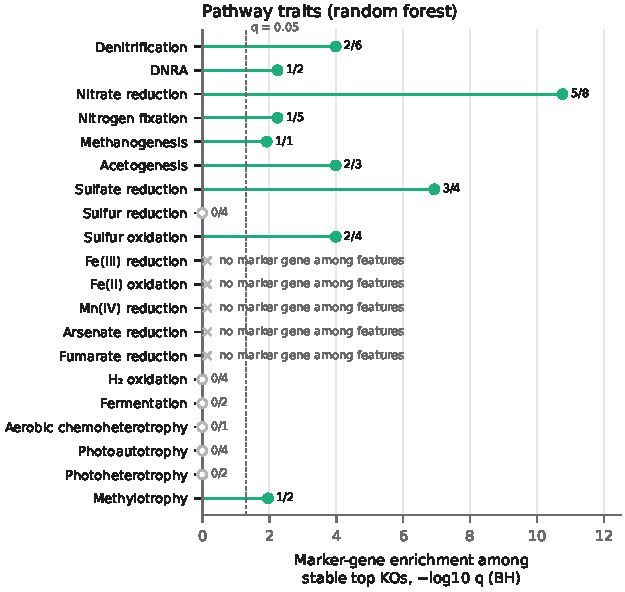
\includegraphics[width=0.55\linewidth,height=\textheight,keepaspectratio,alt={Top features of the pathway models and their agreement with known markers. Enrichment of marker genes among the most stable features of random forests for the 20 pathway traits. Grey points mark traits without significant enrichment, and crosses traits without a marker among the features. Labels such as 2/6 count marker genes among these features.}]{figures/FigS1_xai_pathways.pdf}
\caption{\textbf{Top features of the pathway models and their agreement
with known markers.} Enrichment of marker genes among the most stable
features of random forests for the 20 pathway traits. Grey points mark
traits without significant enrichment, and crosses traits without a
marker among the features. Labels such as 2/6 count marker genes among
these features.}\label{fig:s_pathways}
\end{figure}

\begin{figure}
\centering
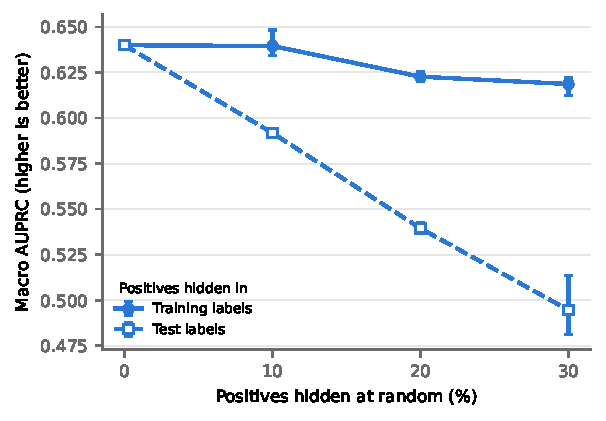
\includegraphics[width=0.6\linewidth,height=\textheight,keepaspectratio,alt={Effect of unreported positives. Positive labels were hidden at random in the training genomes before training or in the test genomes at scoring. Macro AUPRC of a random forest on the KO panel (300 trees, one seed) in genus-level cross-validation, averaged over folds within each category, so higher than in Table . Error bars show the range of three repeats.}]{figures/FigS2_label_noise.pdf}
\caption{\textbf{Effect of unreported positives.} Positive labels were
hidden at random in the training genomes before training or in the test
genomes at scoring. Macro AUPRC of a random forest on the KO panel (300
trees, one seed) in genus-level cross-validation, averaged over folds
within each category, so higher than in Table \ref{tab:cv}. Error bars
show the range of three repeats.}\label{fig:s_noise}
\end{figure}

}

\makeatletter
\newcommand{\authorcontribheading}{%
  \subsection*{Author contributions}%
  \global\let\authorcontribheading\@empty
  \global\def\authorcontribend{.}%
}
\newcommand{\authorcontribsep}{\global\def\authorcontribsep{;\space}}
\newcommand{\authorcontribend}{}
\makeatother
\authorcontribheading\authorcontribsep Shuichi Kawashima:\,Writing --
original draft\authorcontribheading\authorcontribsep Danil
Ezhov:\,Methodology, Software, Formal analysis, Investigation,
Validation, Data curation, Visualization, Writing -- original draft
(prediction sections), Writing -- review \&
editing\authorcontribheading\authorcontribsep Akira R
Kinjo:\,Conceptualization, Writing -- review \&
editing\authorcontribheading\authorcontribsep Julia
Koblitz:\,Conceptualization, Writing -- review \&
editing\authorcontribheading\authorcontribsep Takeru
Nakazato:\,Conceptualization, Writing -- review \&
editing\authorcontribheading\authorcontribsep Yoko
Okabbepu:\,Conceptualization, Writing -- review \&
editing\authorcontribheading\authorcontribsep Risa
Otsuka:\,Conceptualization, Writing -- review \&
editing\authorcontribend

\printbibliography



\end{document}
